%%%%%%%%%%%%%%%%%%%%%%%%%%%%%%%%%%%%%%%%%%%%%%%%
%\newpage
We evaluate here the performance of multiple rational approximation methods over an extensive collection of Zolotarev topologies from \cite{trefethen2024computation}. Specifically, we compare the LF with AAA, AAA with sign, and AAA with sign, damping, and 200 Lawson iterations. In every case, the rational approximation order $r$ of the figure similar to \cref{fig:intro:1a} is selected by setting the lowest relative singular value threshold of the LF to $10^{-14}$, then the same objective is used for the other methods. Then, similarly to \cref{fig:intro:1a_time}, the Zolotarev ratio and computation time are reported for increasing orders $r$. In most cases, we note that the LF leads to an approximant in the form $R_{r-1,r}$ while AAA and its variants are in the form $R_{r,r}$.

\subsection{Case \texttt{'1b'}}

\Cref{fig:1b} involves the classical sign function; it illustrates another symmetric case, i.e., a configuration where Z4 poles and zeros are aligned along the vertical axis, and Z3 poles and zeros are  necessarily real. In this case, the LF normalized singular values below the threshold indicate an approximation order of $r=18$. Then we use this order for each approximation method. By inspecting \cref{fig:1b}, the Zolotarev number indicates that AAA with sign and Lawson provides better results in almost all cases. LF performs better when orders are fairly high and also performs better than AAA and AAA signed. In addition, in this very simple case, the computation time of AAA and AAA with sign is below the LF. AAA with Lawson needs substantially more time.

\begin{figure}[H]
    \centering
    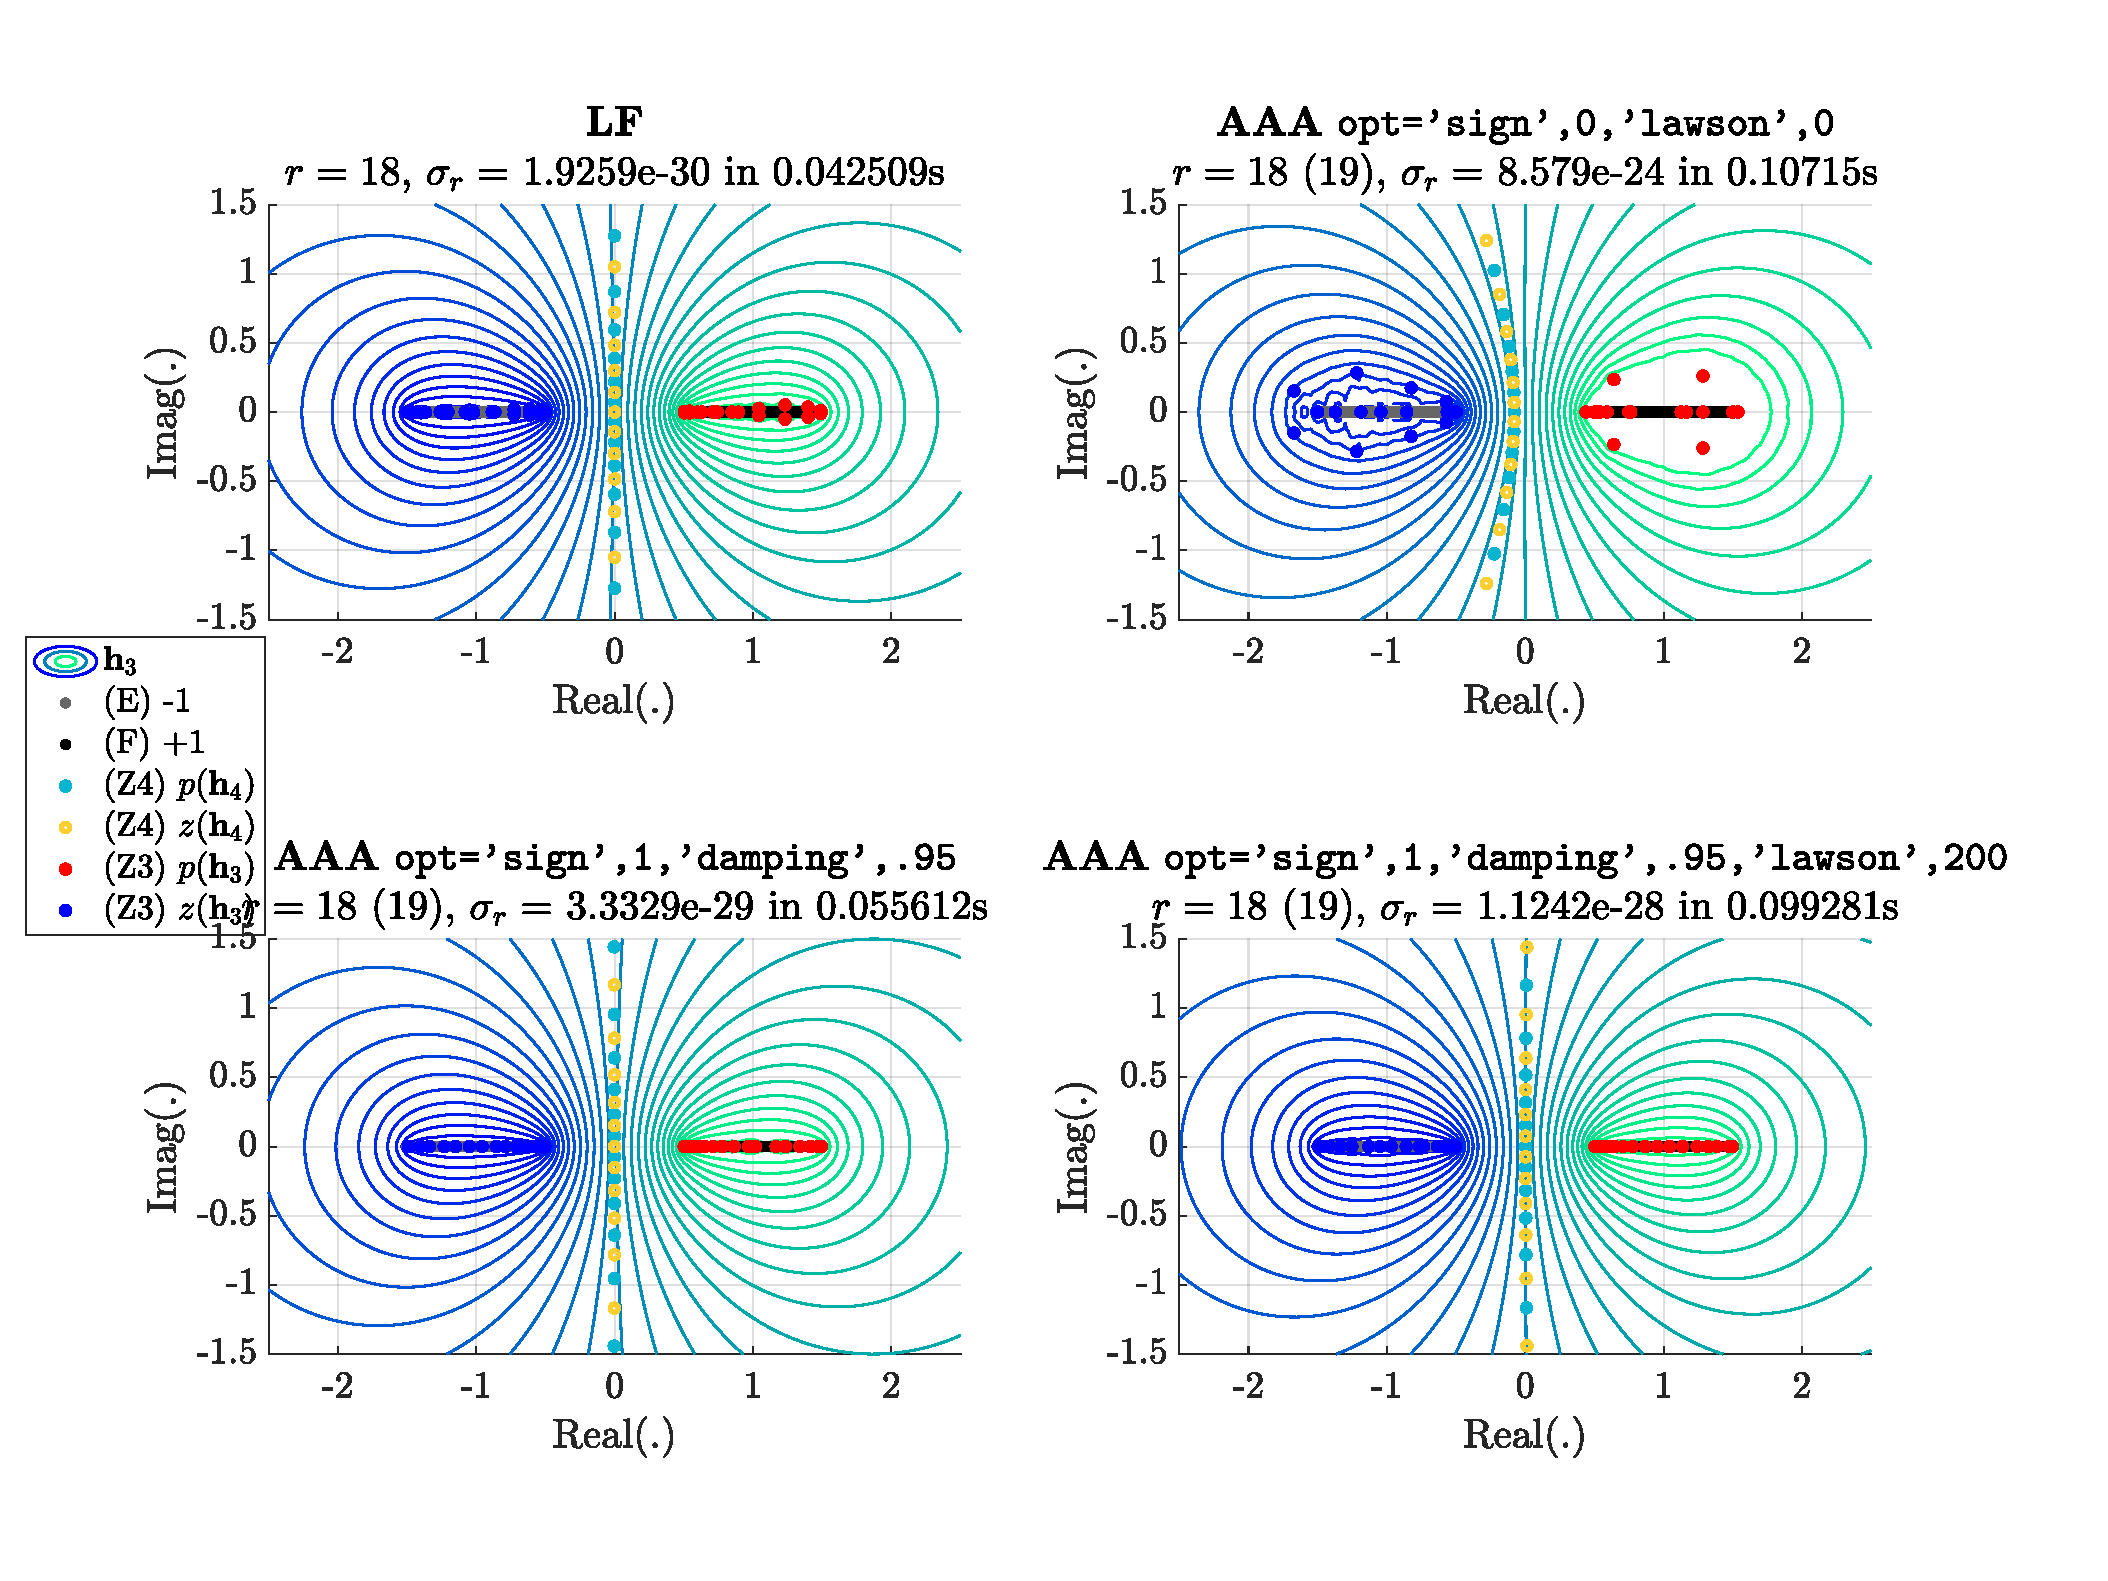
\includegraphics[width=.75\textwidth]{figures/all/cas_1b_r1e-14.pdf}
    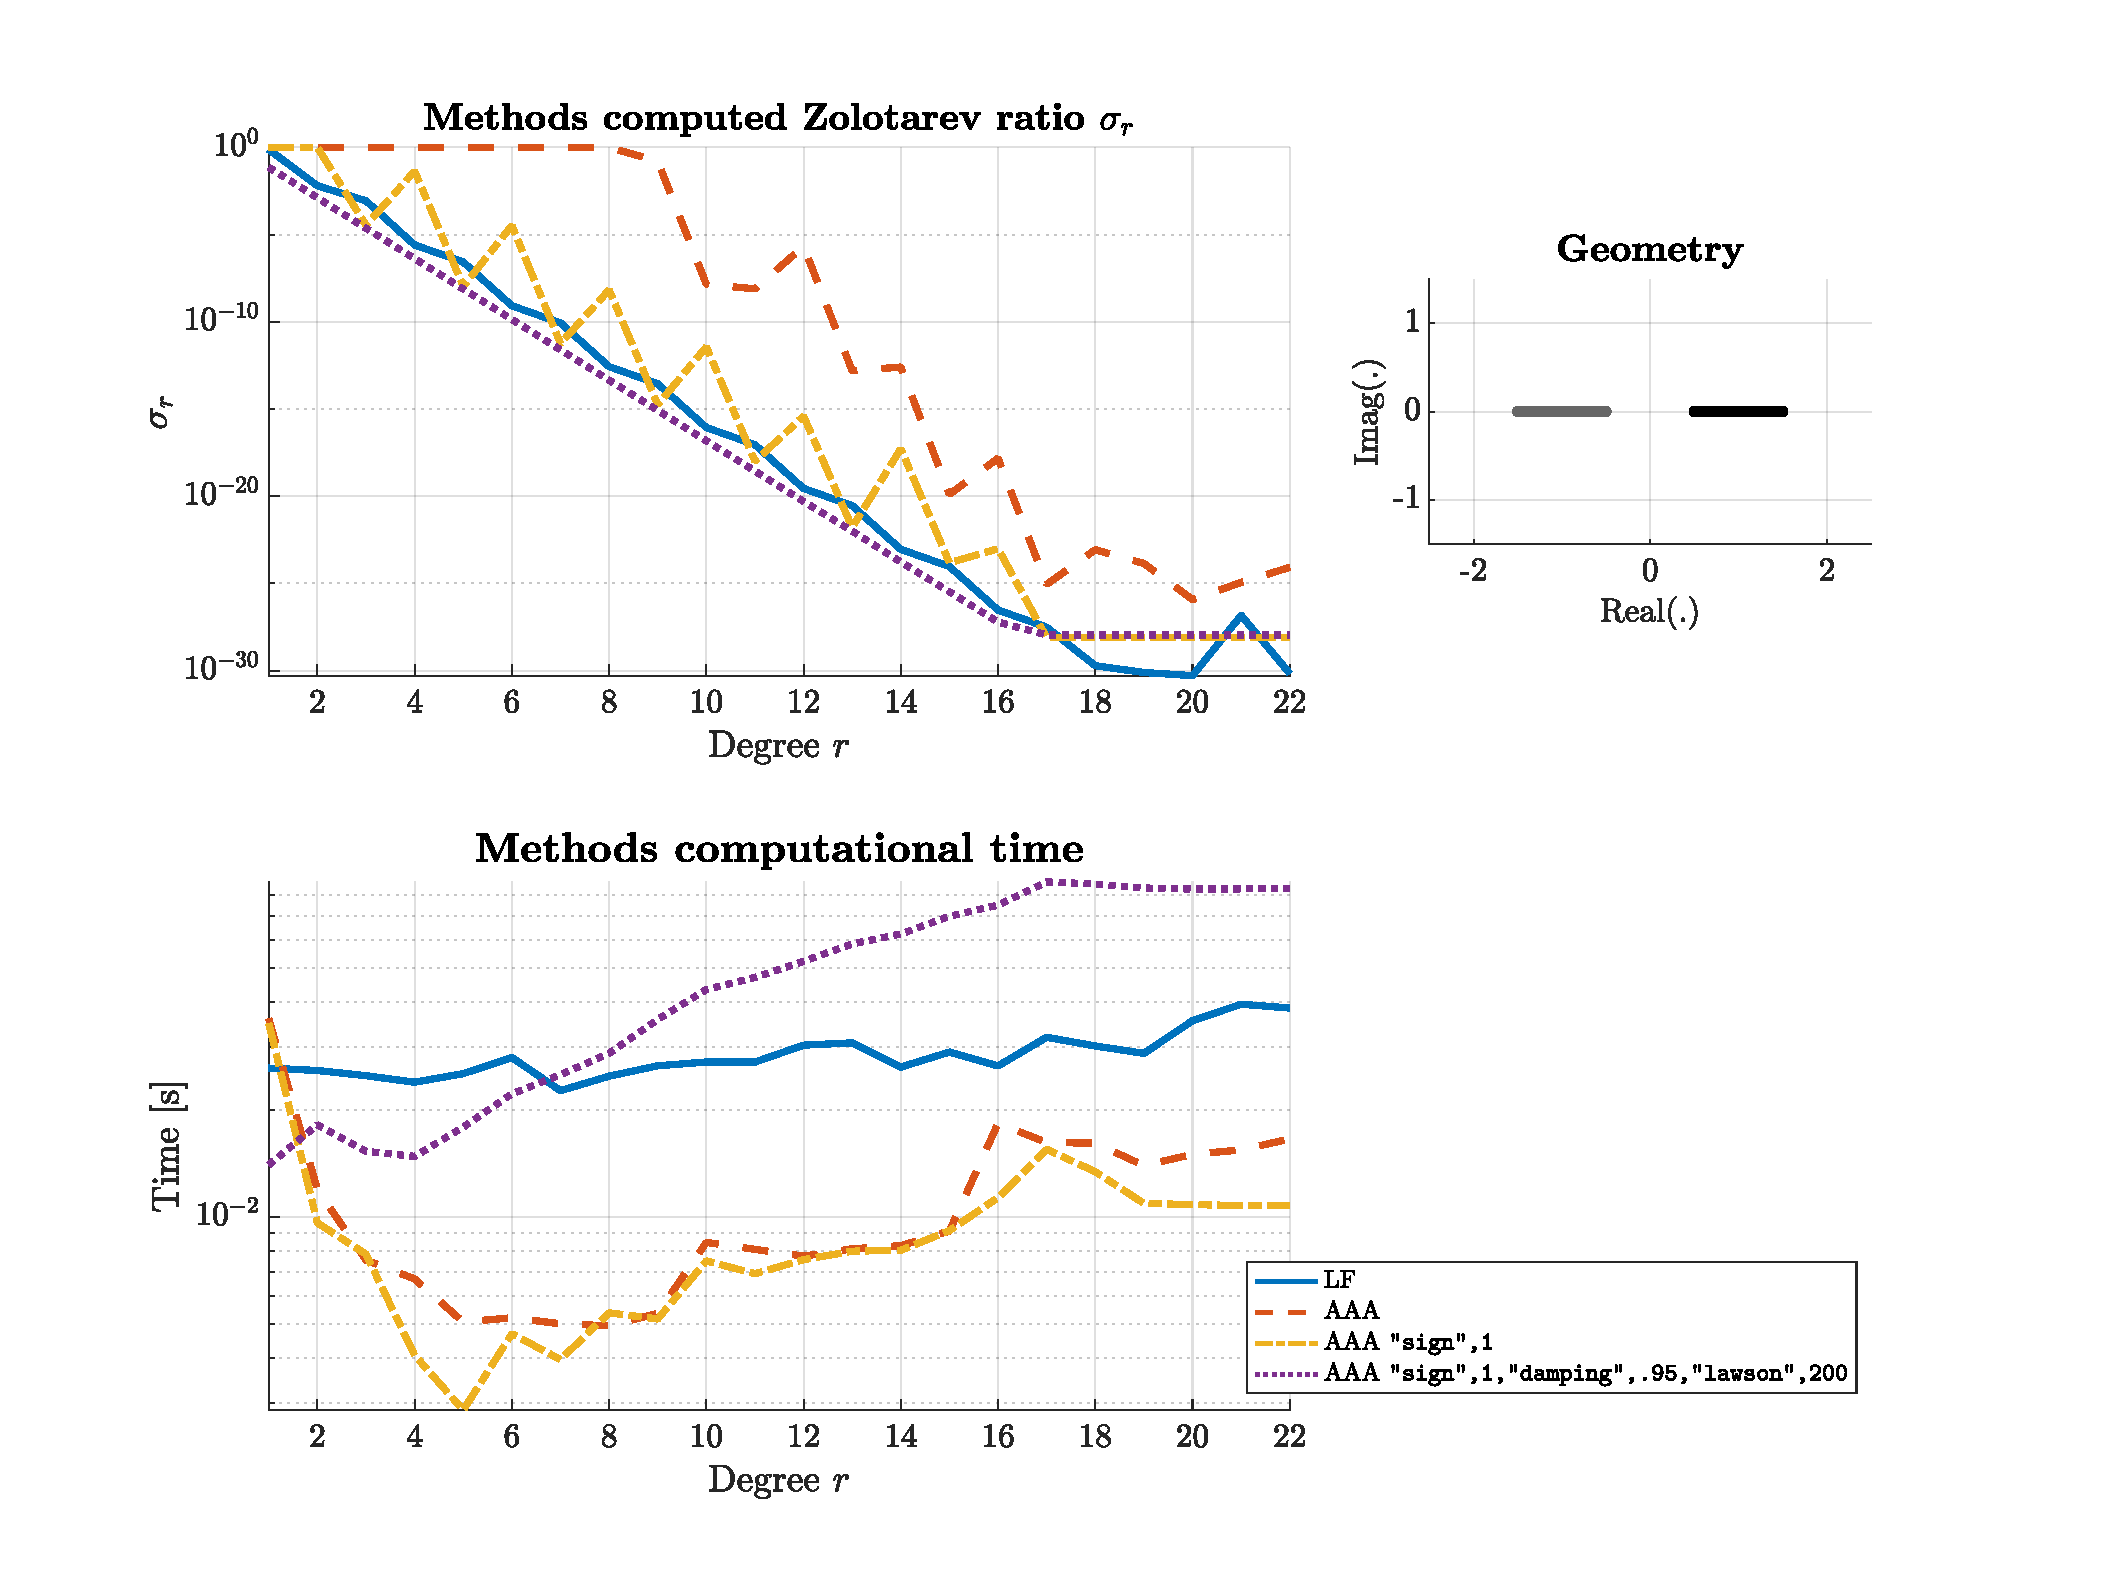
\includegraphics[width=.75\textwidth]{figures/time_accuracy/cas_1b_zol_time.pdf}
    \caption{Case \texttt{'1b'}. Top: same description as \cref{fig:intro:1a}. Bottom: same description as \cref{fig:intro:1a_time}.}
    \label{fig:1b}
\end{figure}


%%%%%%%%%%%%%%%%%%%%%%%%%%%%%%%%%%%%%%%%%%%%%%%%
\newpage
\subsection{Case \texttt{'1c'}}

\Cref{fig:1c} illustrates a non-symmetric case, i.e., a configuration where Z4 poles and zeros are not necessarily aligned along the vertical axis, and Z3 poles and zeros are not necessarily real and complex conjugated. In this case, the LF normalized singular values below the threshold indicate an approximation order of $r=24$. Then we apply this order to each approximation method. By inspecting  \cref{fig:1c} the Zolotarev number indicates that AAA with sign and AAA with sign and Lawson provides better results in almost all cases. LF outperforms the other methods when orders are fairly high.  In addition, in this simplified case, the computation time of AAA and AAA with sign is below the LF. AAA with Lawson needs substantially more time.

\begin{figure}[H]
    \centering
    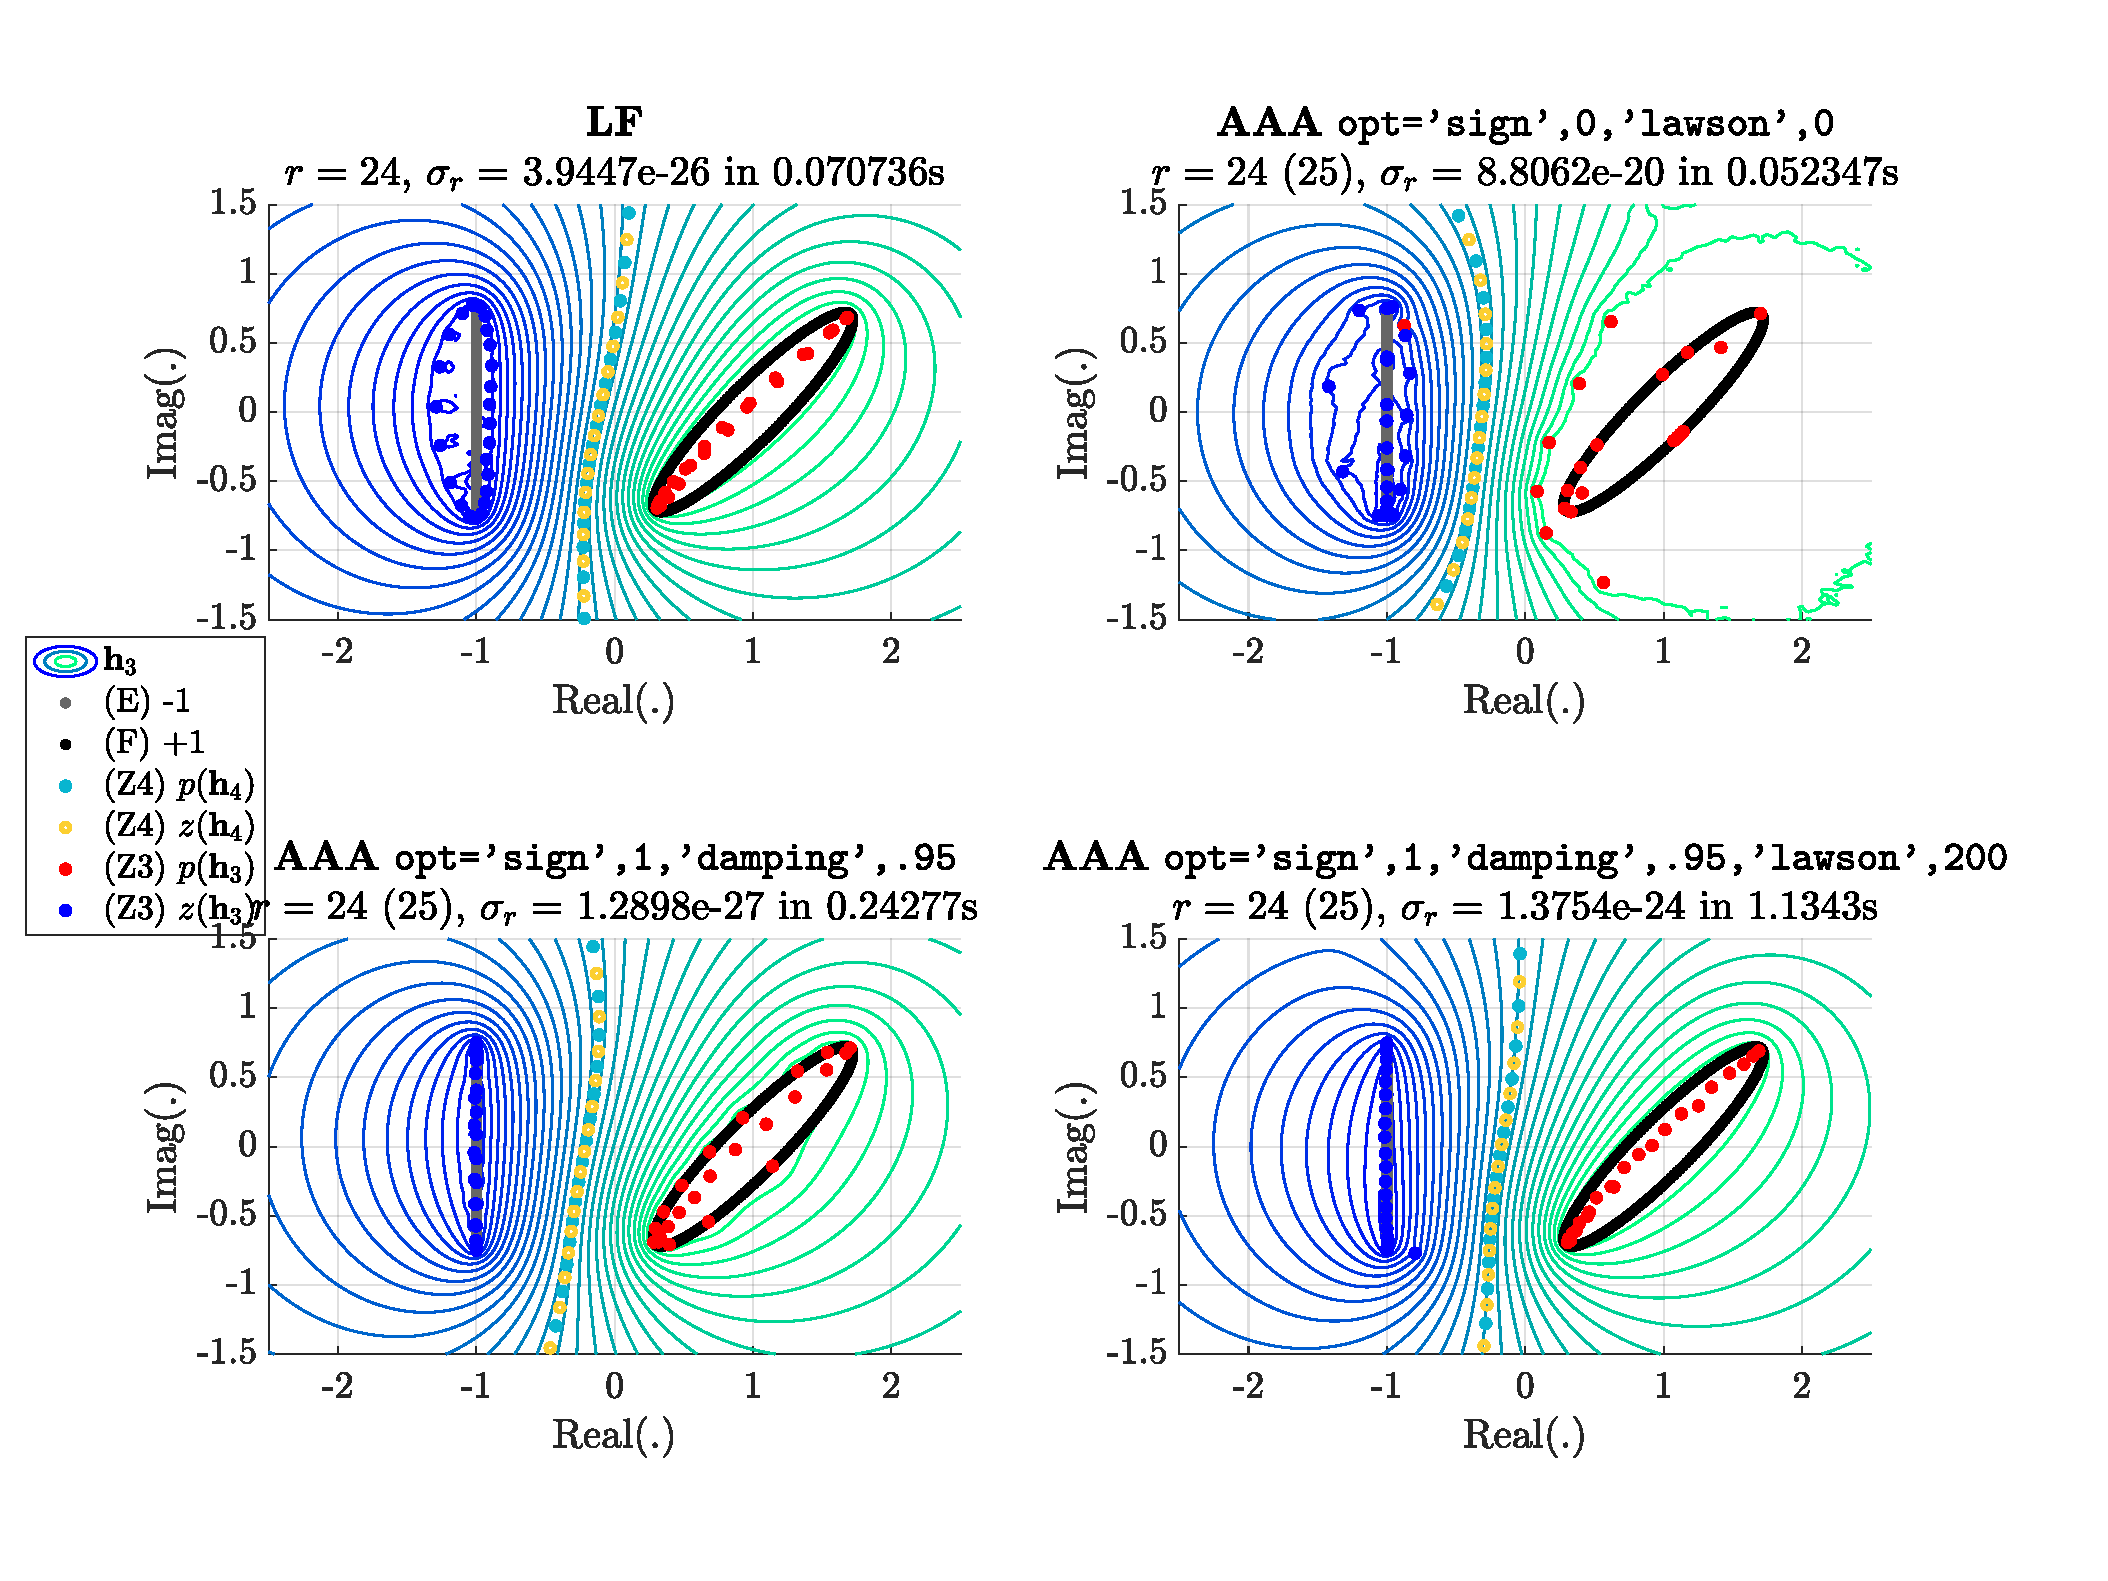
\includegraphics[width=.75\textwidth,align=c]{figures/all/cas_1c_r1e-14.pdf}
    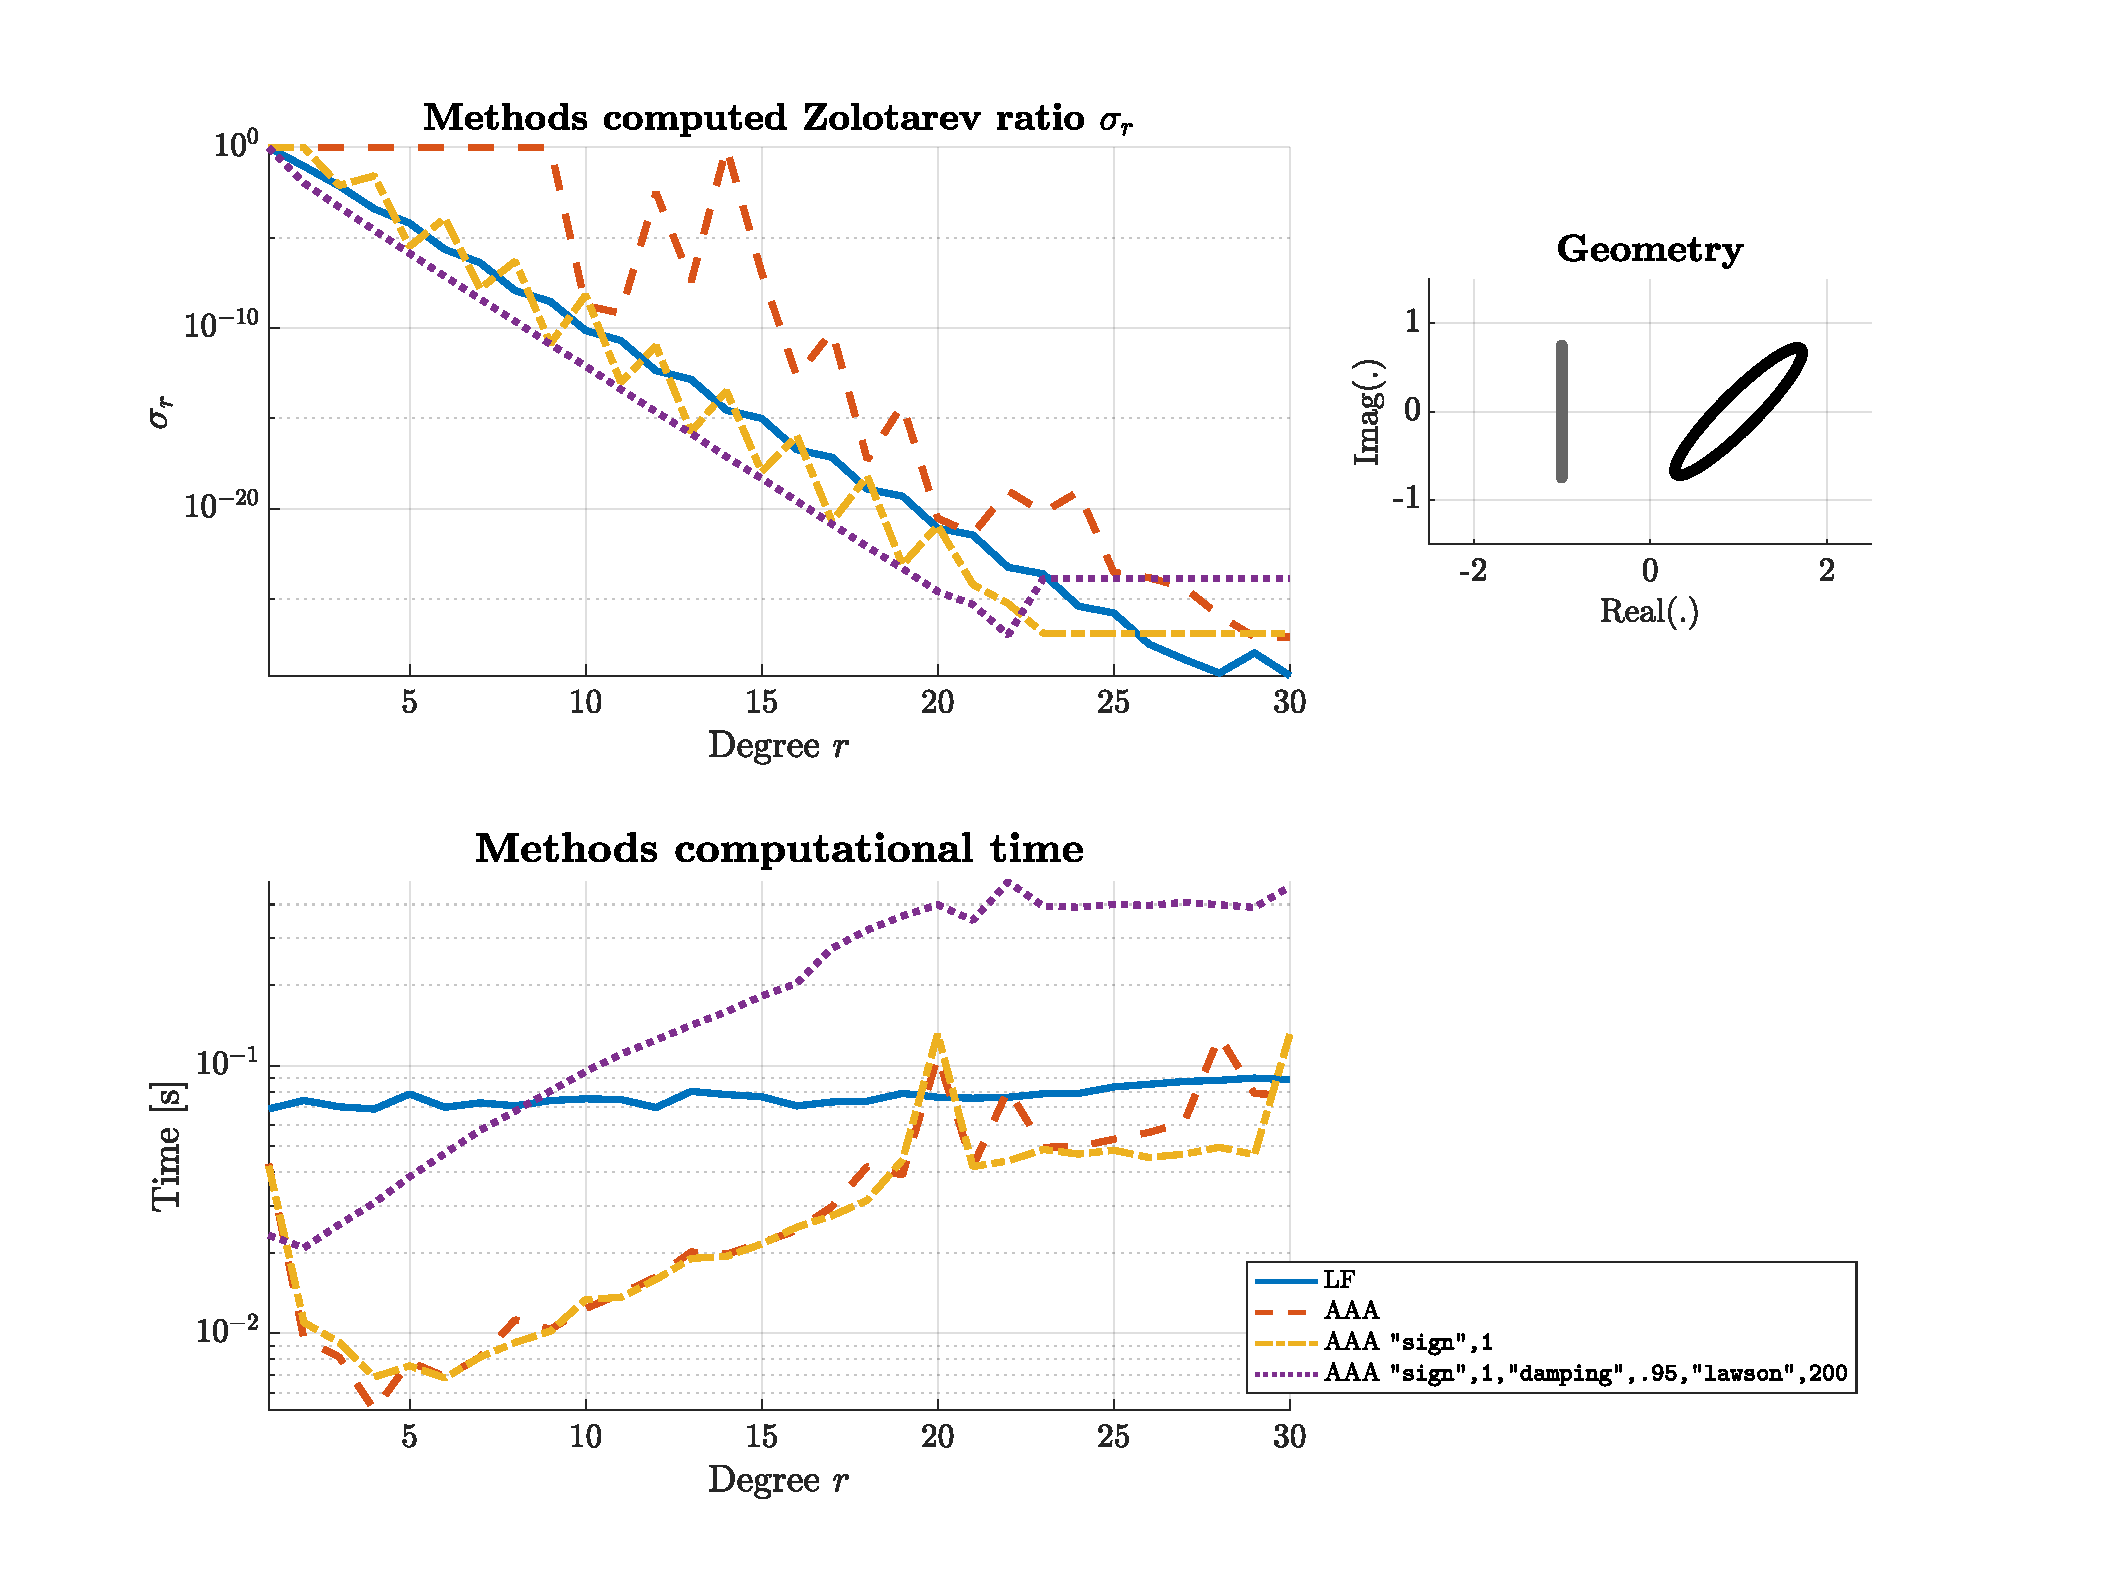
\includegraphics[width=.75\textwidth,align=c]{figures/time_accuracy/cas_1c_zol_time.pdf}
    \caption{Case \texttt{'1c'}. Top: same description as \cref{fig:intro:1a}. Bottom: same description as \cref{fig:intro:1a_time}.}
    \label{fig:1c}
\end{figure}

%%%%%%%%%%%%
\newpage
\subsection{Case \texttt{'1d'}}

This example considers a configuration symmetric by rotation. In \cref{fig:1d}, the time and accuracy plots indicate similar results in terms of Zolotarev number for LF, AAA sign, and AAA sign Lawson, with a slight advantage to AAA sign Lawson for almost all orders, except for high  approximation orders where LF outperforms. Moreover, inspecting the computation time rapidly shows an advantage of the LF. By inspecting the upper frame, only the LF and AAA sign result in poles and zeros totally separated and distributed along the yin/yang geometry. The two others show poles and zeros in the wrong part of the domain. 

\begin{figure}[H]
    \centering
    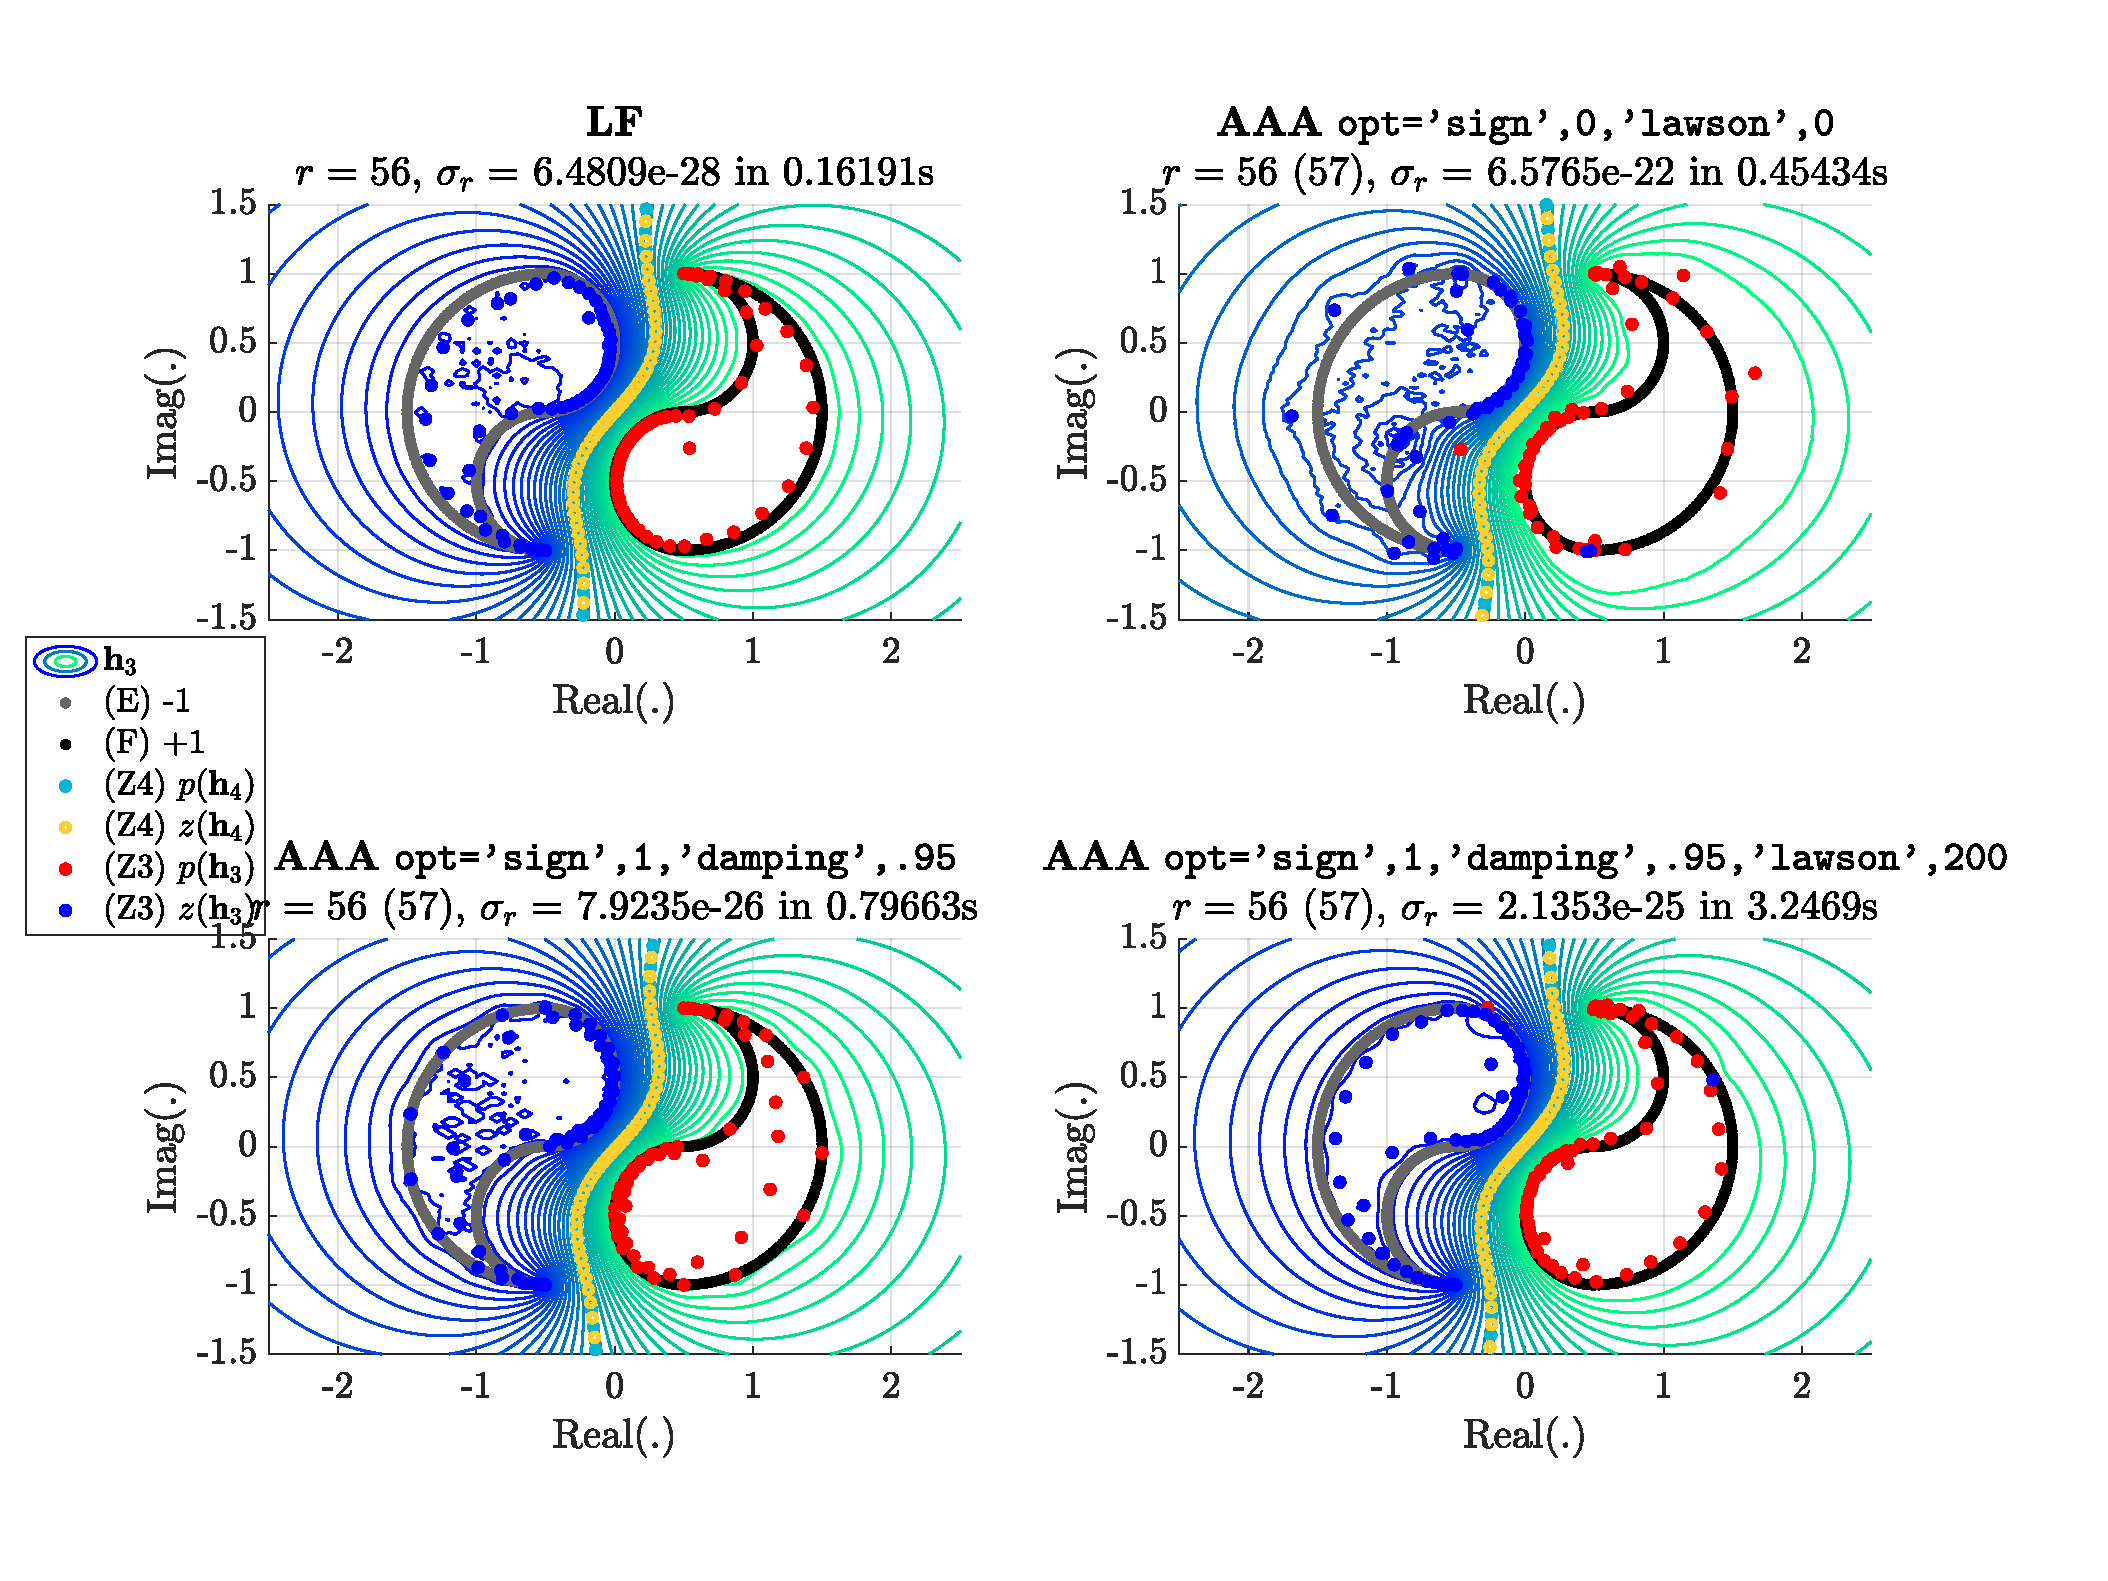
\includegraphics[width=.75\textwidth,align=c]{figures/all/cas_1d_r1e-14.pdf}
    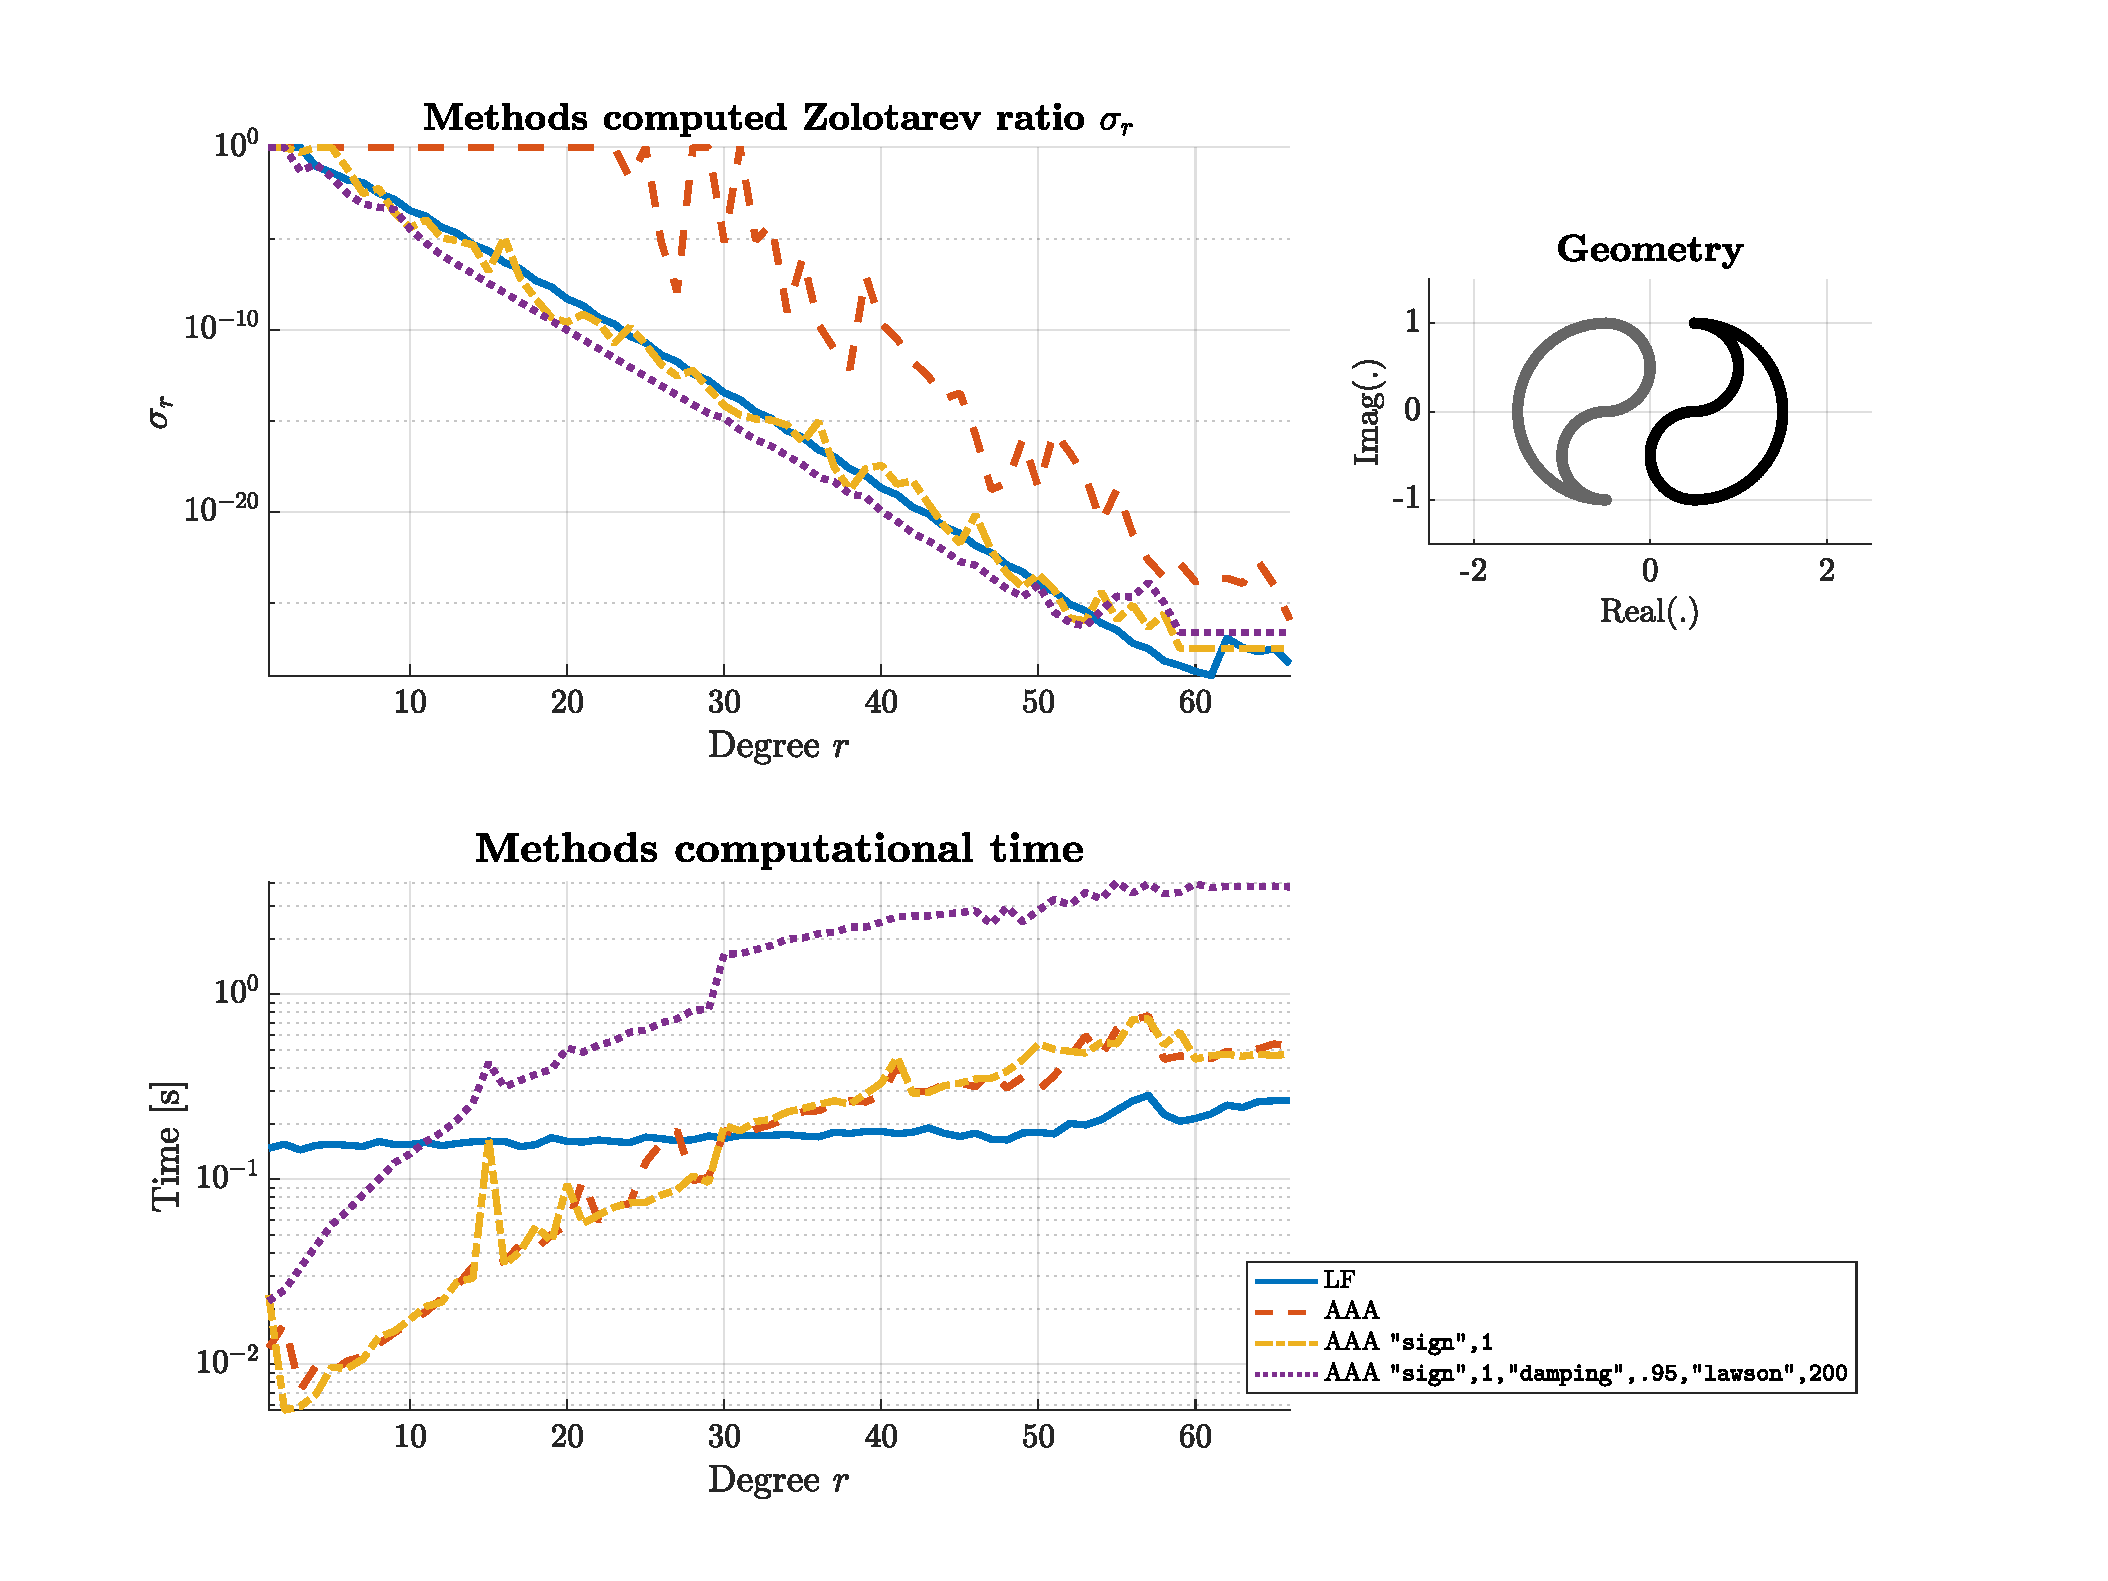
\includegraphics[width=.75\textwidth,align=c]{figures/time_accuracy/cas_1d_zol_time.pdf}
    \caption{Case \texttt{'1d'}. Top: same description as \cref{fig:intro:1a}. Bottom: same description as \cref{fig:intro:1a_time}.}
    \label{fig:1d}
\end{figure}


%%%%%%%%%%%%
\newpage
\subsection{Case \texttt{'2a'}}

This configuration exhibits symmetry with the  horizontal axis. Here again, the Zolotarev number obtained by the AAA sign and the AAA Lawson sign is most of the time lower than the LF. However, similarly to the previous observations and initial discussions, the LF is the only method able to reproduce a perfect complex conjugate collection of poles and zeros for both Z3 and Z4 approximations (see \cref{fig:2a}). This indicates that the structure of the true solution may be recovered by the LF. Note that the symmetry of poles and zeros means that the rational form can be obtained with real-valued polynomials only. Such a feature is relevant in the case where only data values are available, as it discovers the structure. 

\begin{figure}[H]
    \centering
    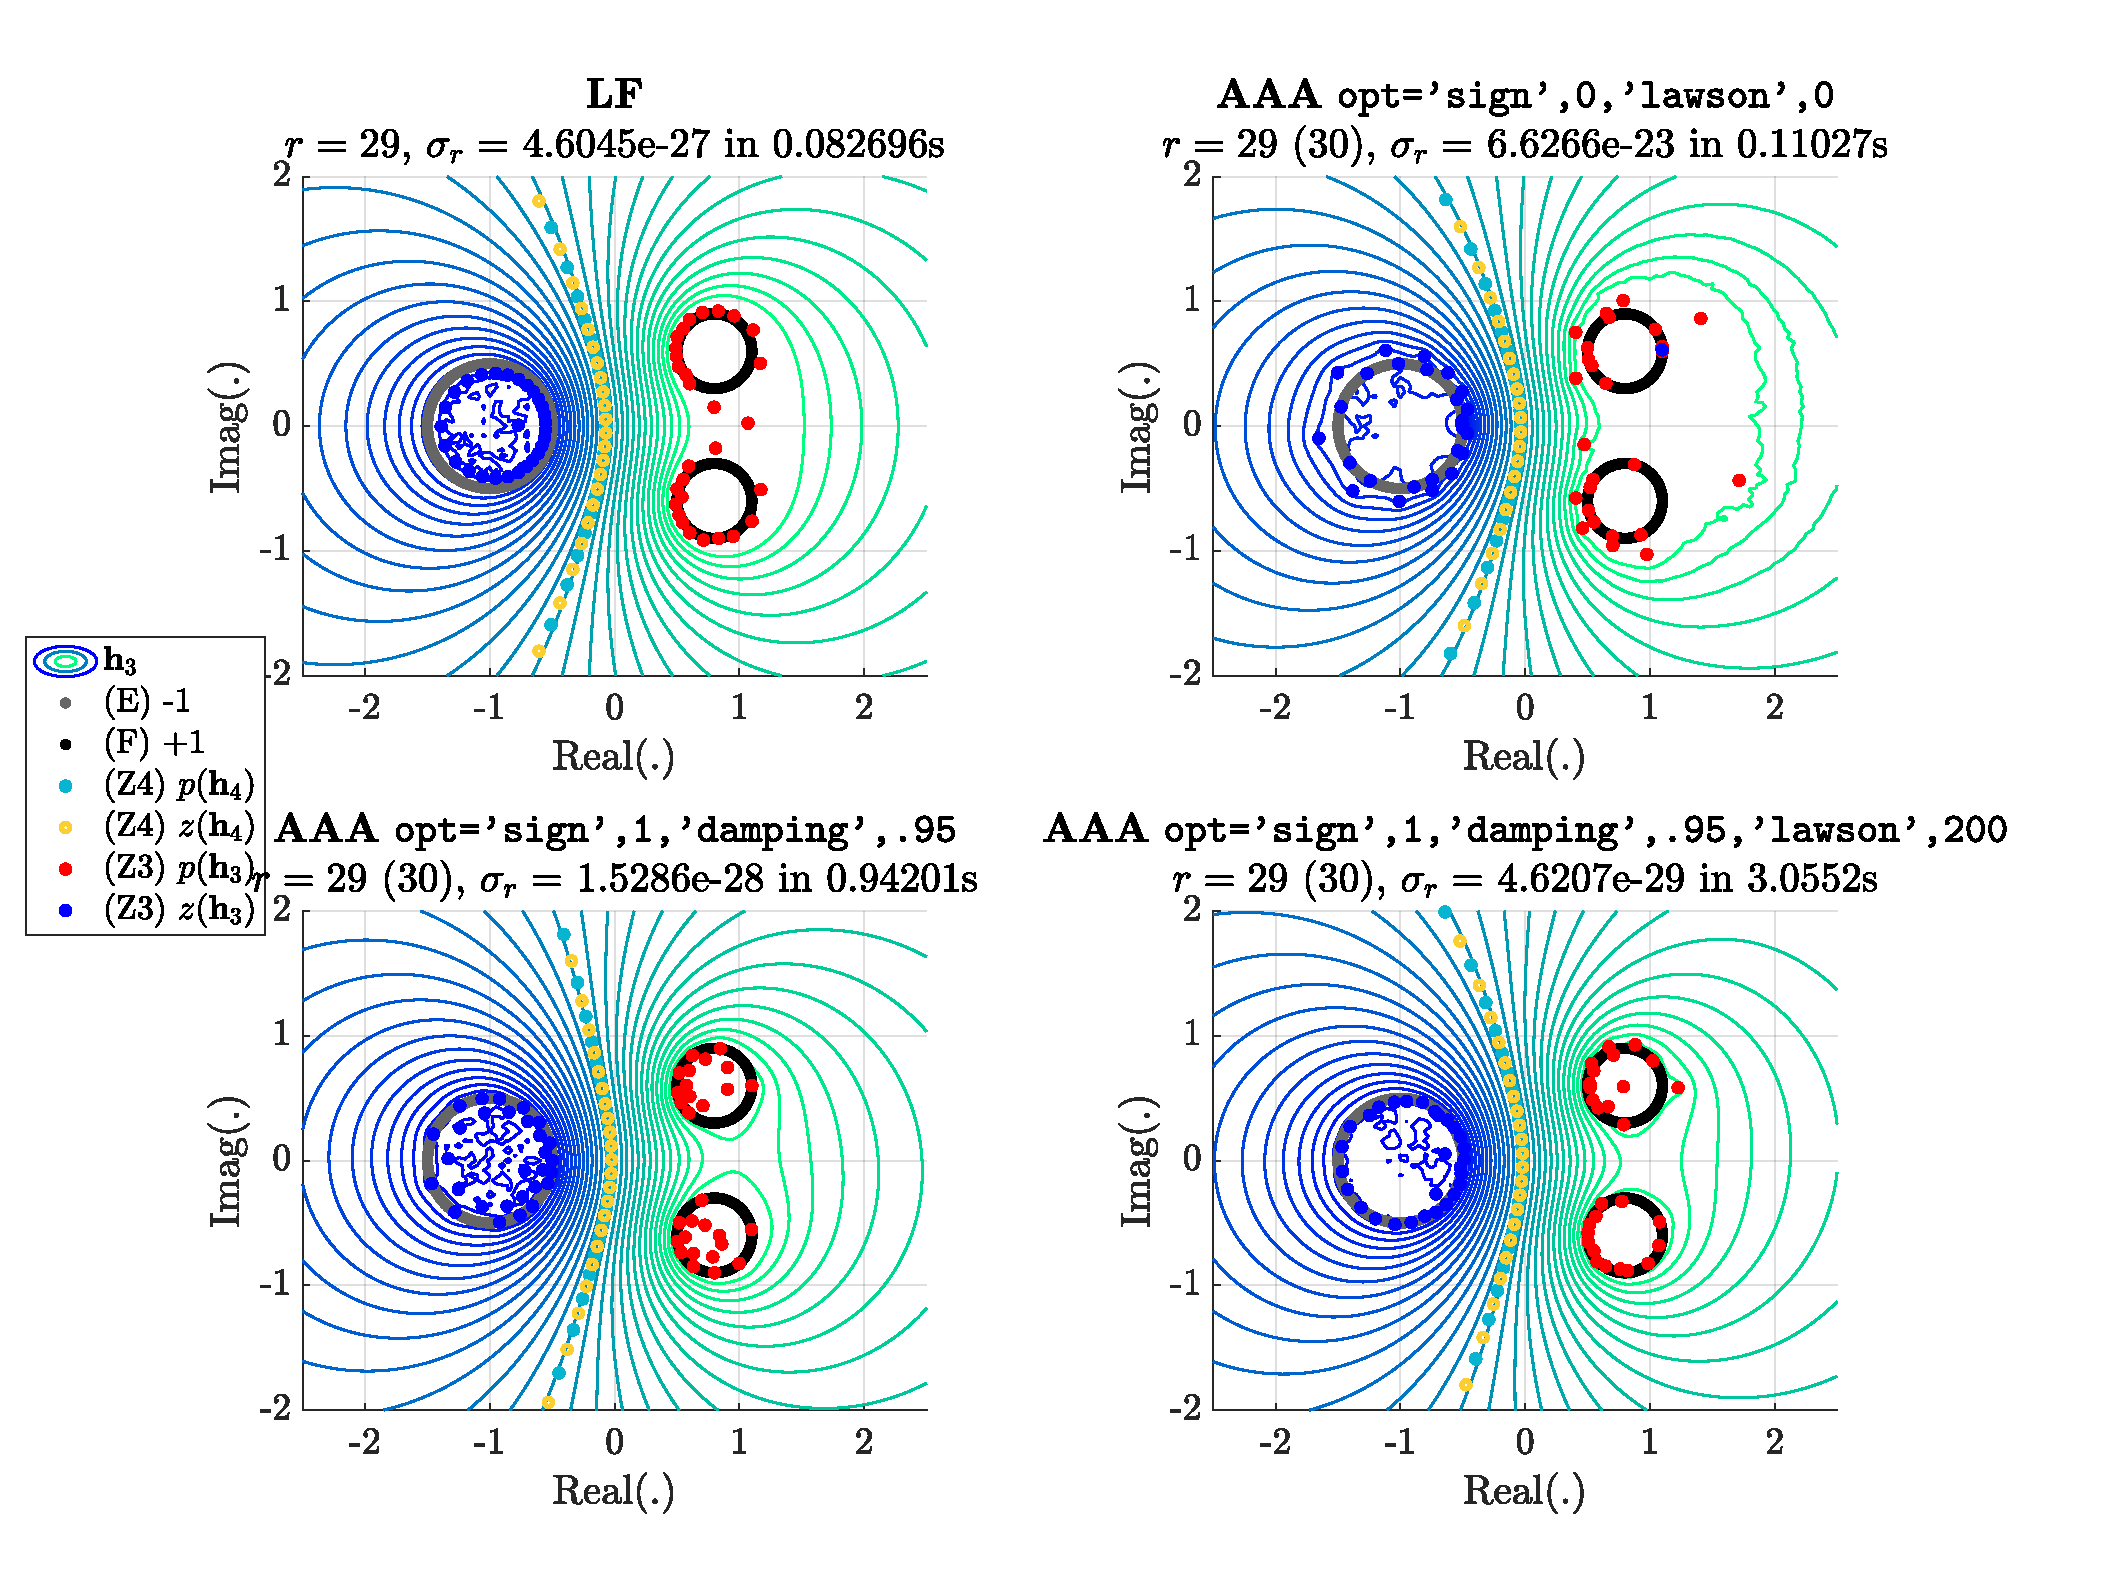
\includegraphics[width=.75\textwidth,align=c]{figures/all/cas_2a_r1e-14.pdf}
    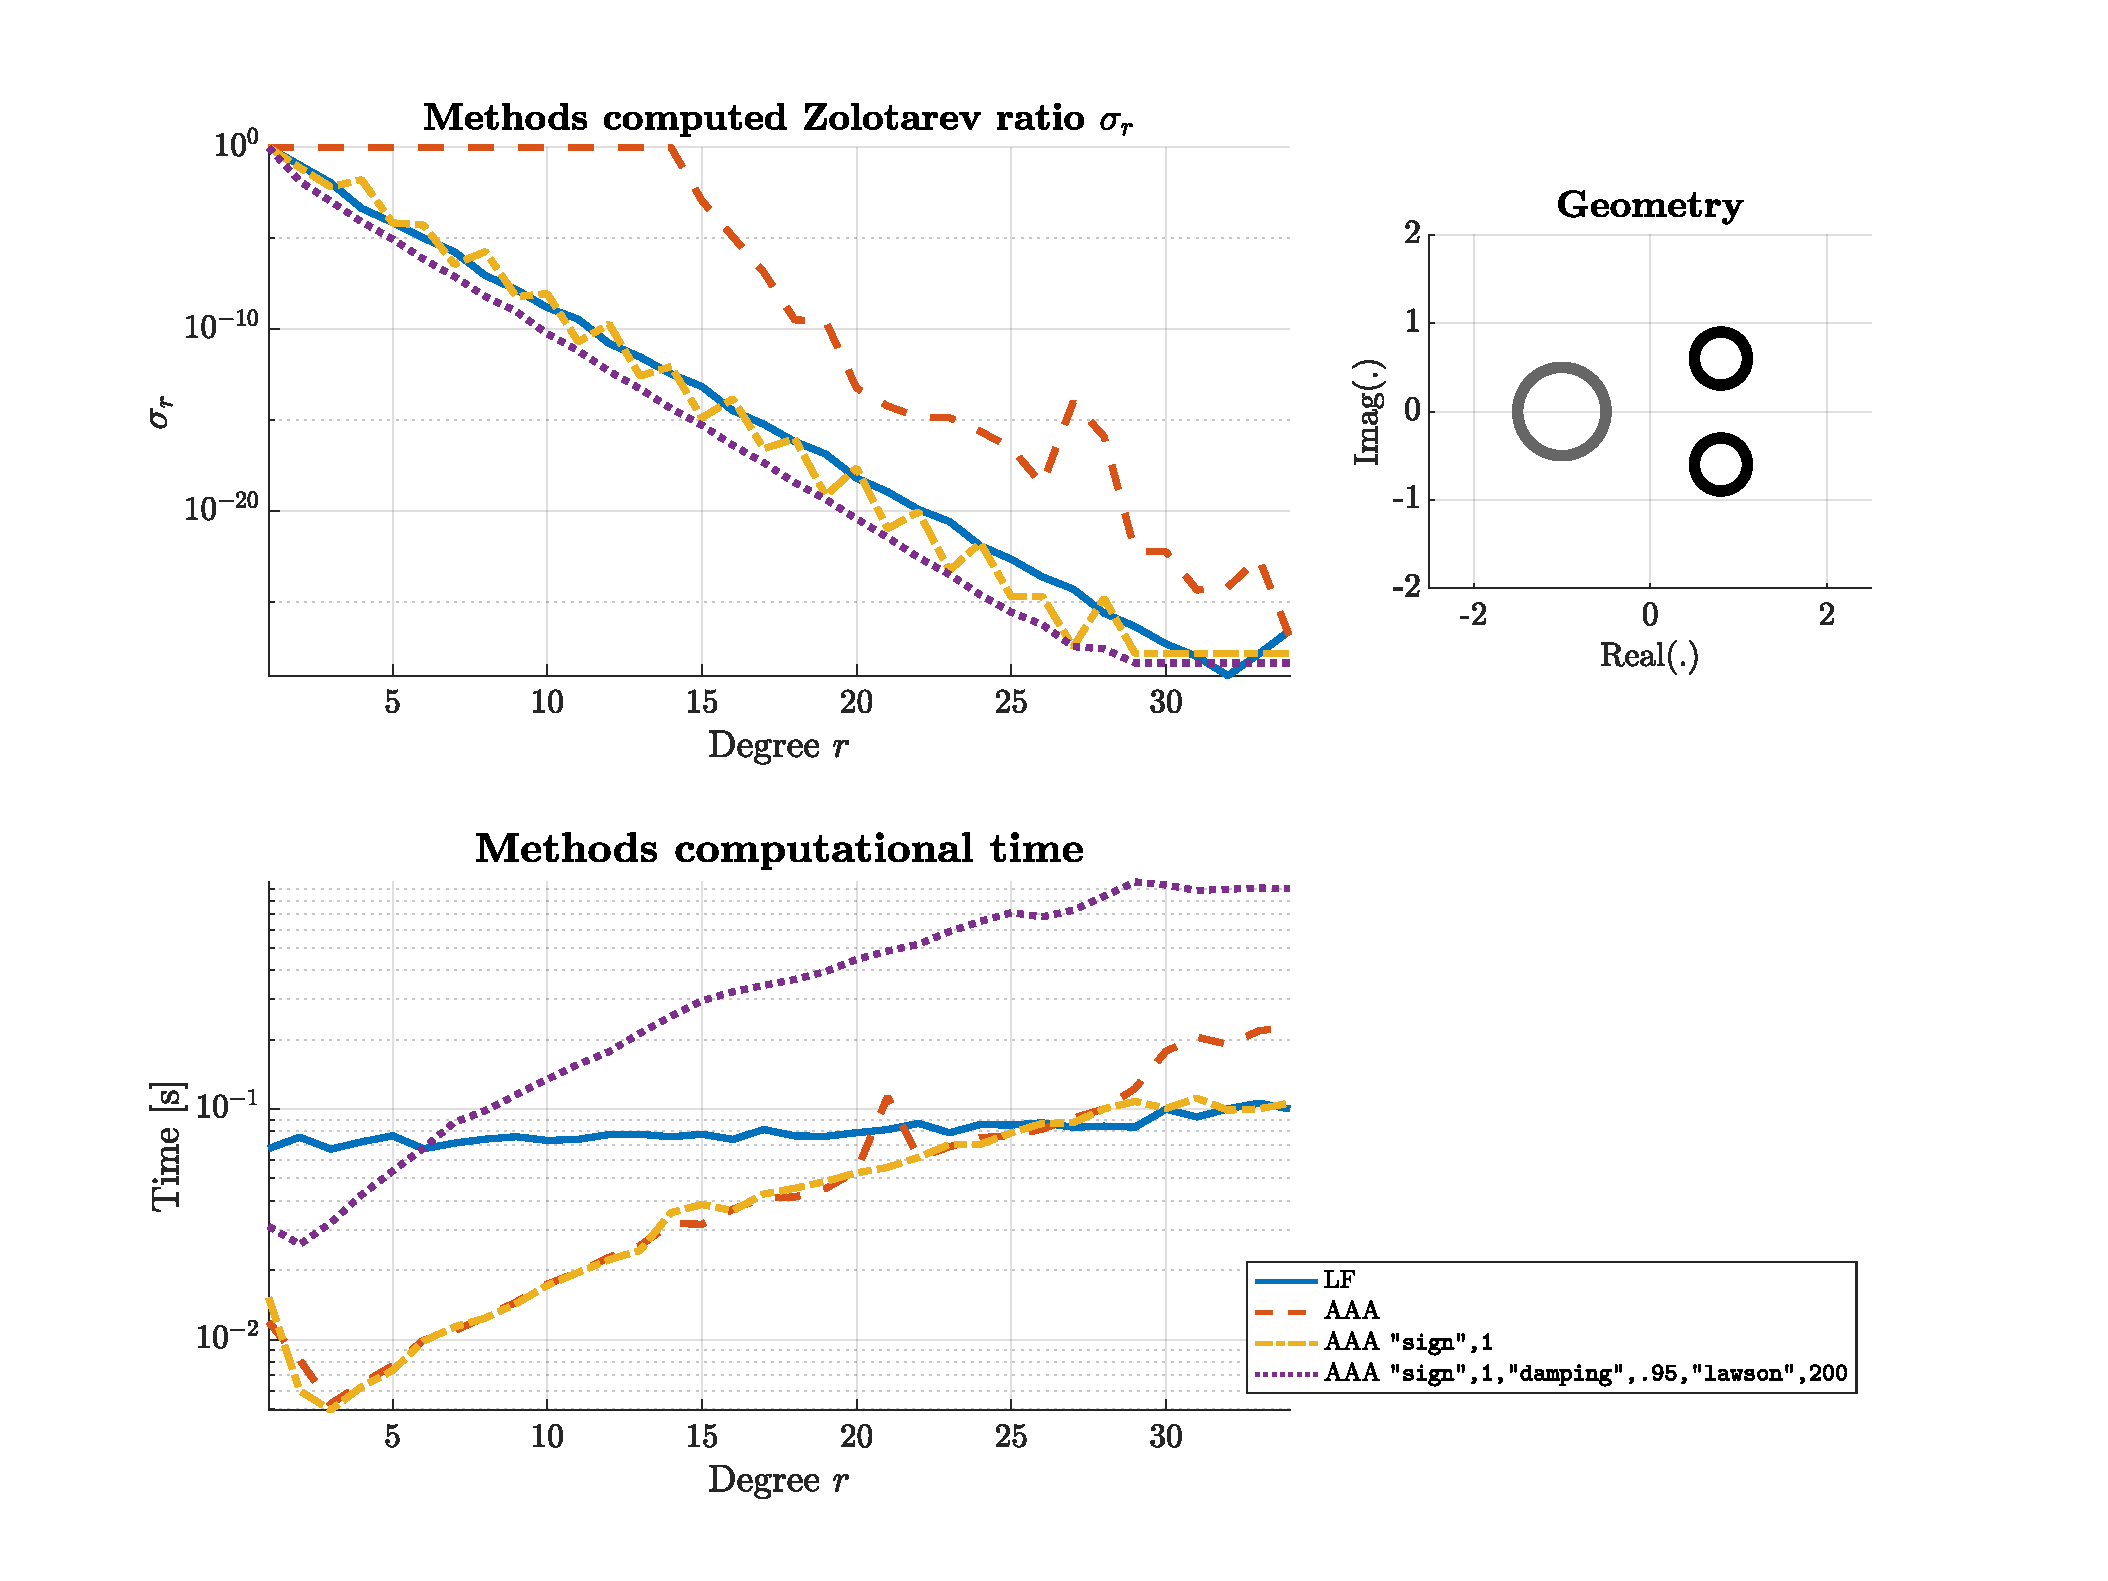
\includegraphics[width=.75\textwidth,align=c]{figures/time_accuracy/cas_2a_zol_time.pdf}
    \caption{Case \texttt{'2a'}. Top: same description as \cref{fig:intro:1a}. Bottom: same description as \cref{fig:intro:1a_time}.}
    \label{fig:2a}
\end{figure}


%%%%%%%%%%%%
\newpage
\subsection{Case \texttt{'2b'}}

This setup is an extension of the real-valued sign function \texttt{'1b'}, with two discontinuities. Same observations as the latter case can be made. The LF provides rather inaccurate results compared to the AAA sign and the AAA sign Lawson. However, the computation time is significantly lower. In this specific setup, the sign and Lawson variants clearly improve the accuracy. This observation is not surprising, as it gives substantial information to the approximation structure. However, by inspecting the upper frame of \cref{fig:2b}, the AAA sign Lawson approach results in poles and zeros with a strange  repartition, symptomatic of spurious poles/zeros distributions. In this upper frame, the LF does not recover a set of only real zeros for Z3; however, the latter are complex and closed by conjugation.

\begin{figure}[H]
    \centering
    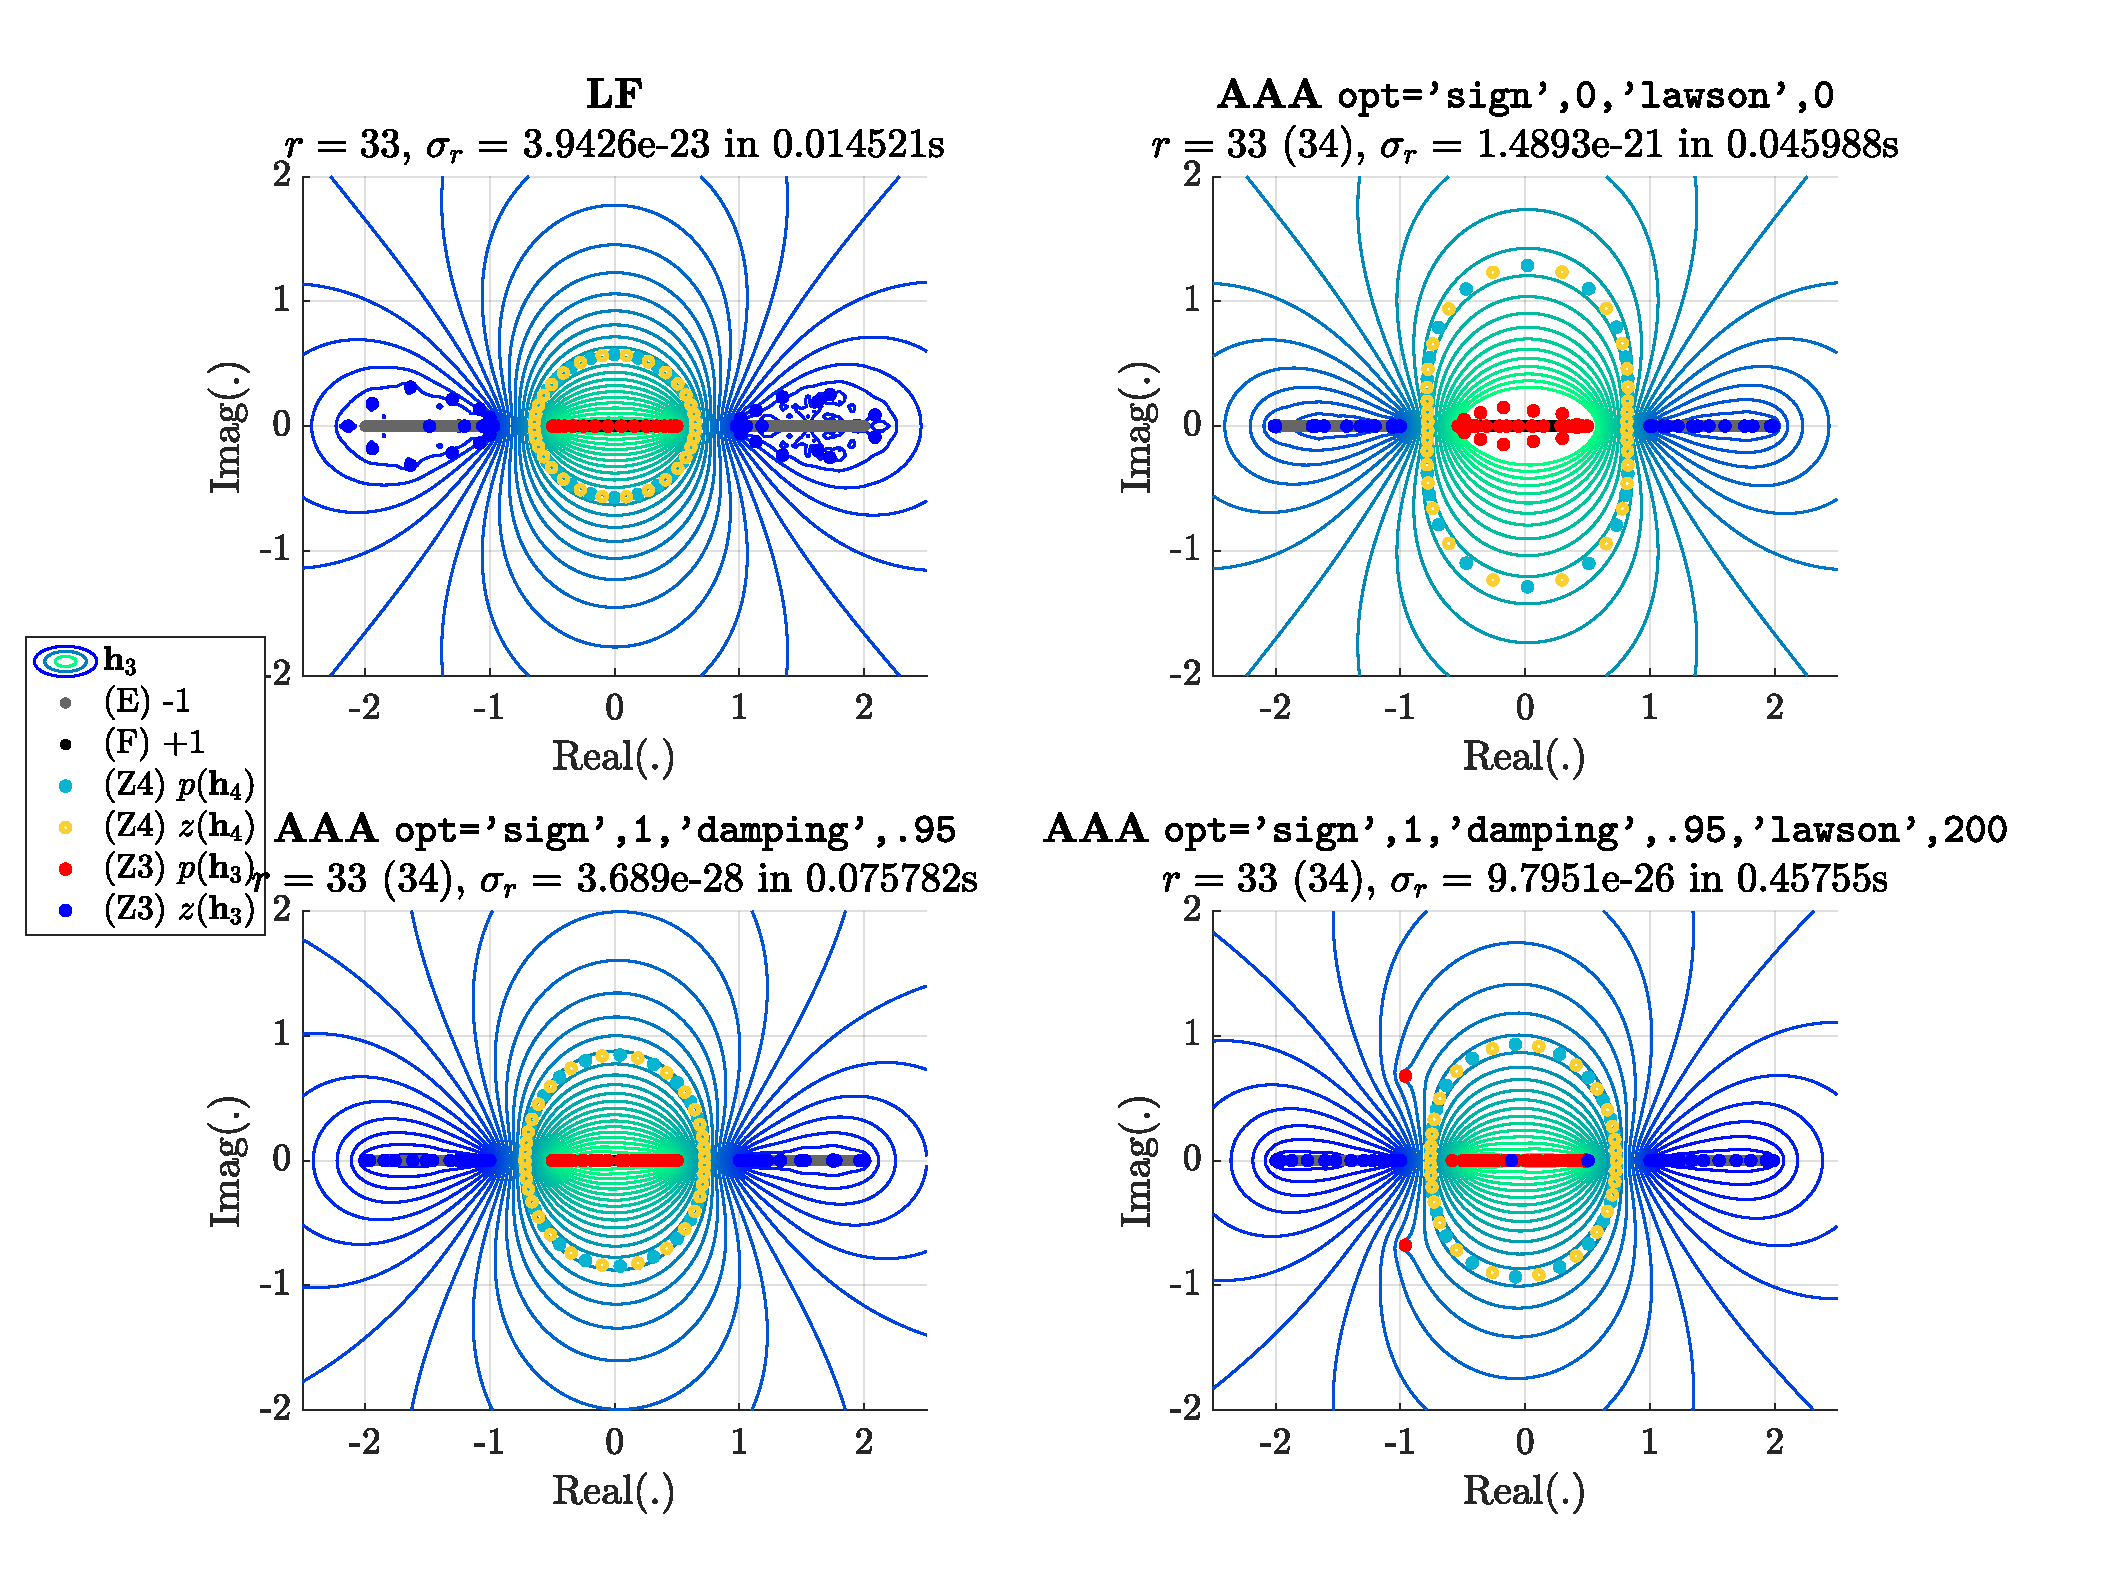
\includegraphics[width=.75\textwidth,align=c]{figures/all/cas_2b_r1e-14.pdf}
    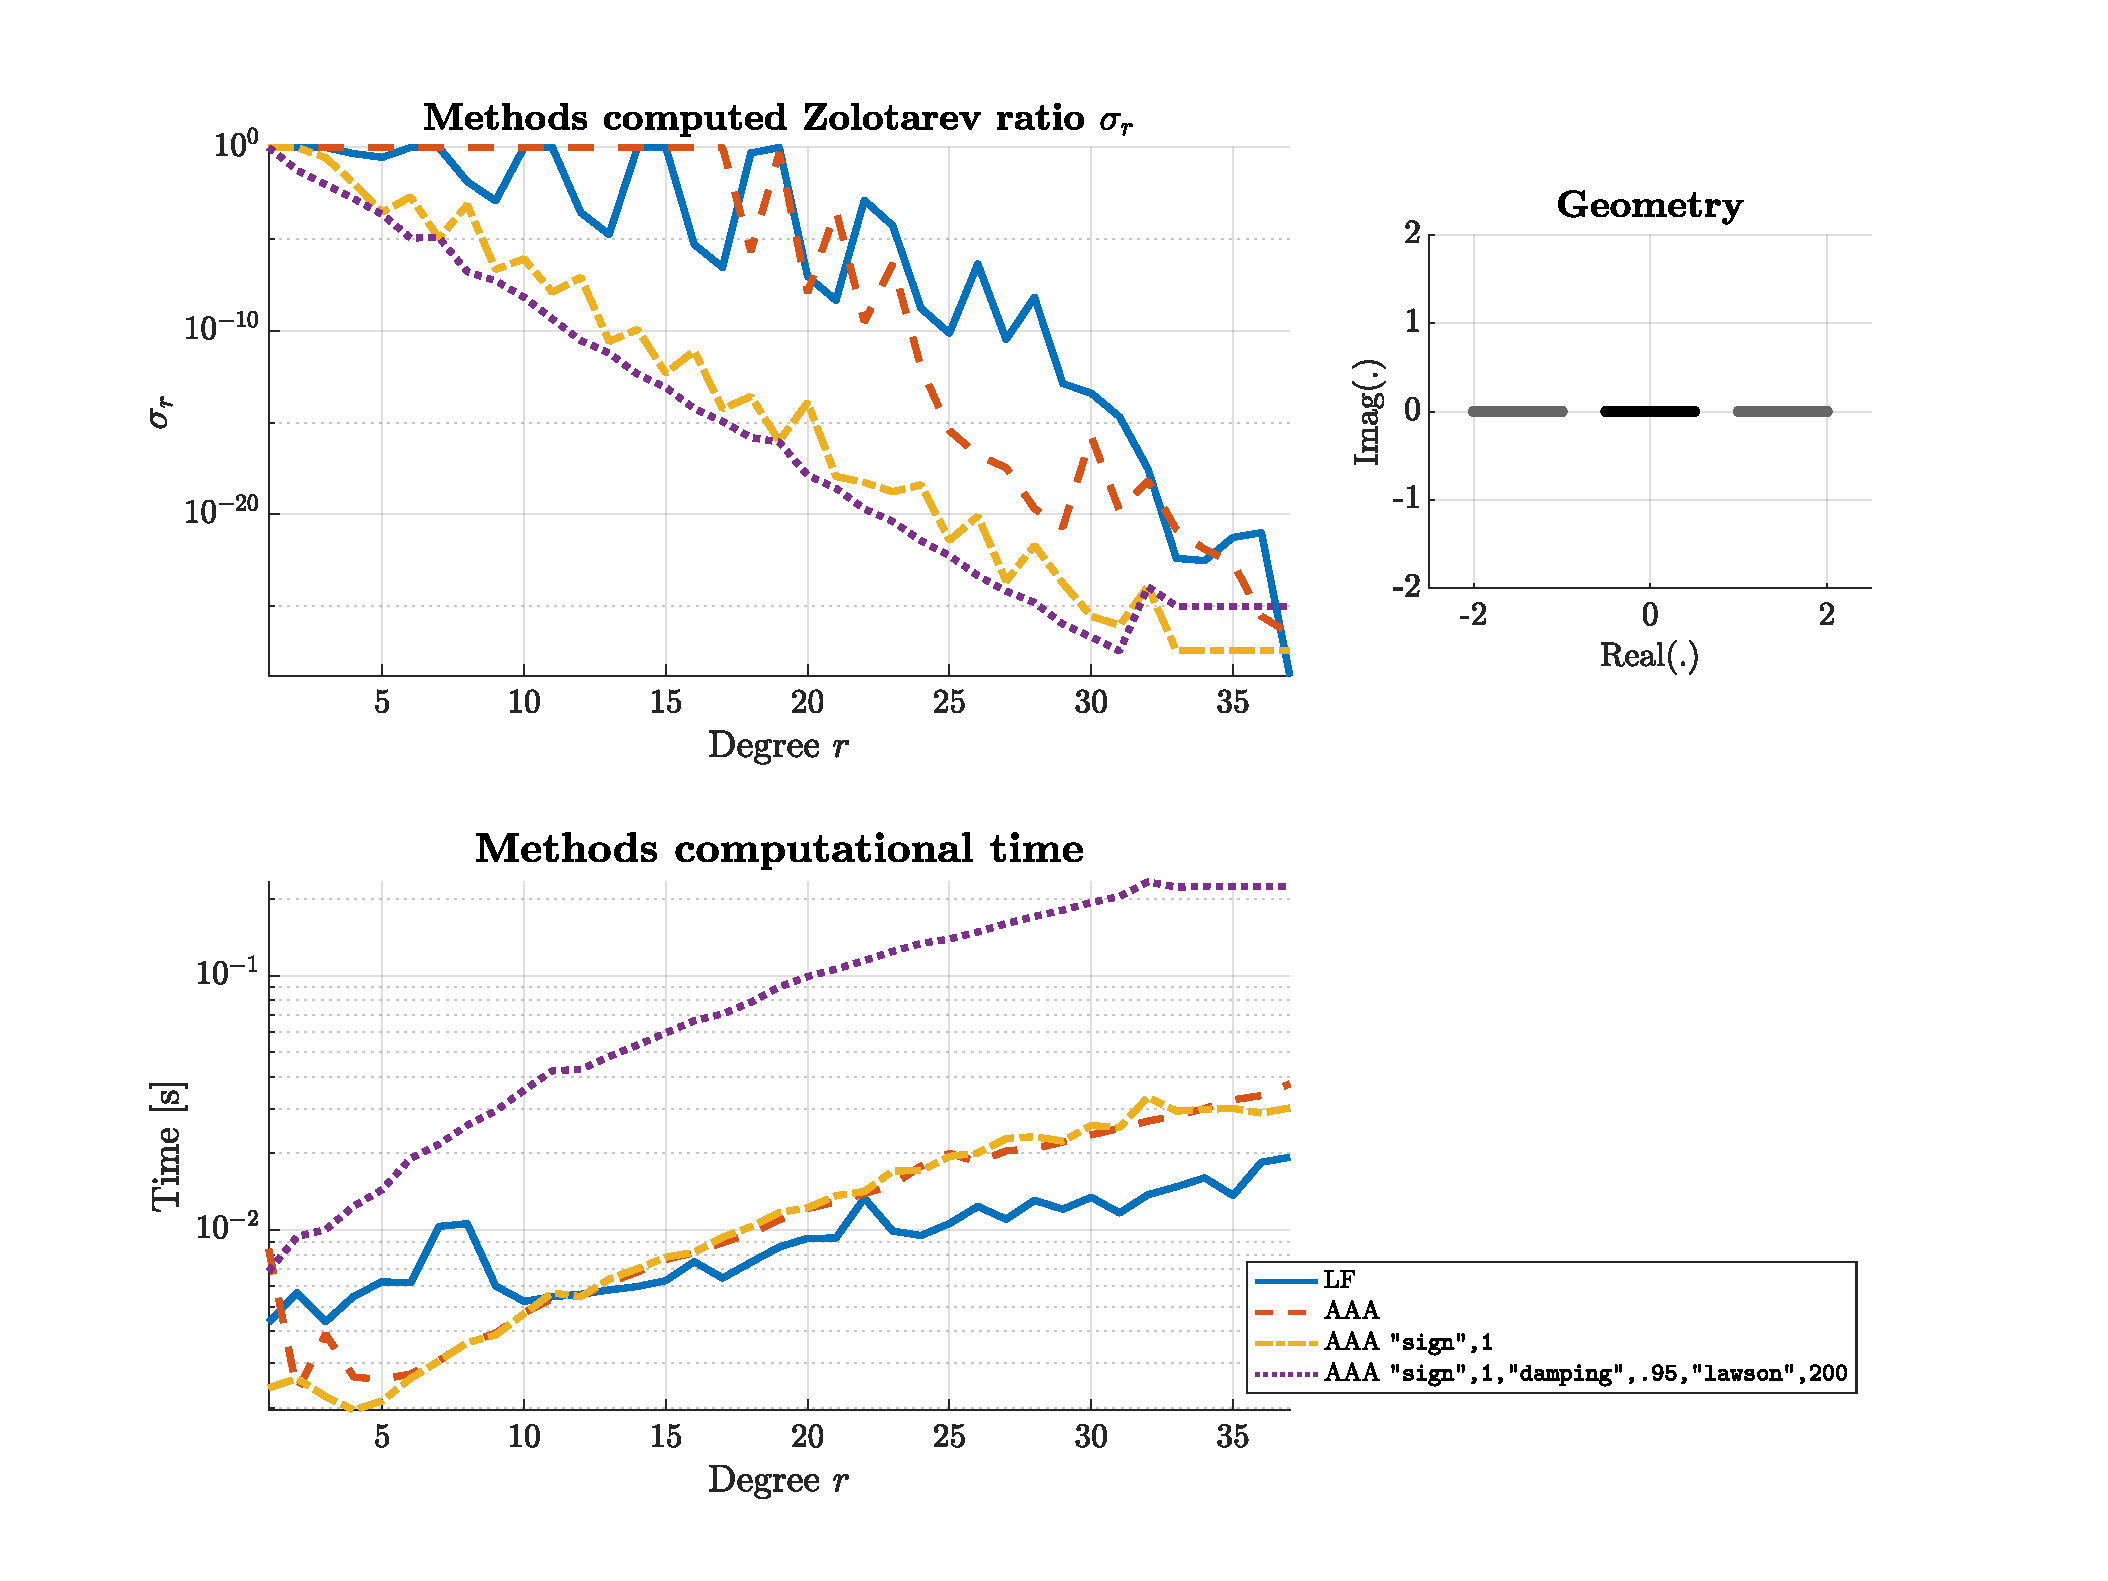
\includegraphics[width=.75\textwidth,align=c]{figures/time_accuracy/cas_2b_zol_time.pdf}
    \caption{Case \texttt{'2b'}. Top: same description as \cref{fig:intro:1a}. Bottom: same description as \cref{fig:intro:1a_time}.}
    \label{fig:2b}
\end{figure}

%%%%%%%%%%%%
\newpage
\subsection{Case \texttt{'2c'}}

This non-symmetric case illustrates a configuration where LF outperforms all other methods in both accuracy (see lower frame in \cref{fig:2c}). Once again, the AAA sign Lawson setup leads Z3 approximation  to poles and zeros peculiarly located with singularities and zeros in the non-expected area (top right and bottom right).

\begin{figure}[H]
    \centering
    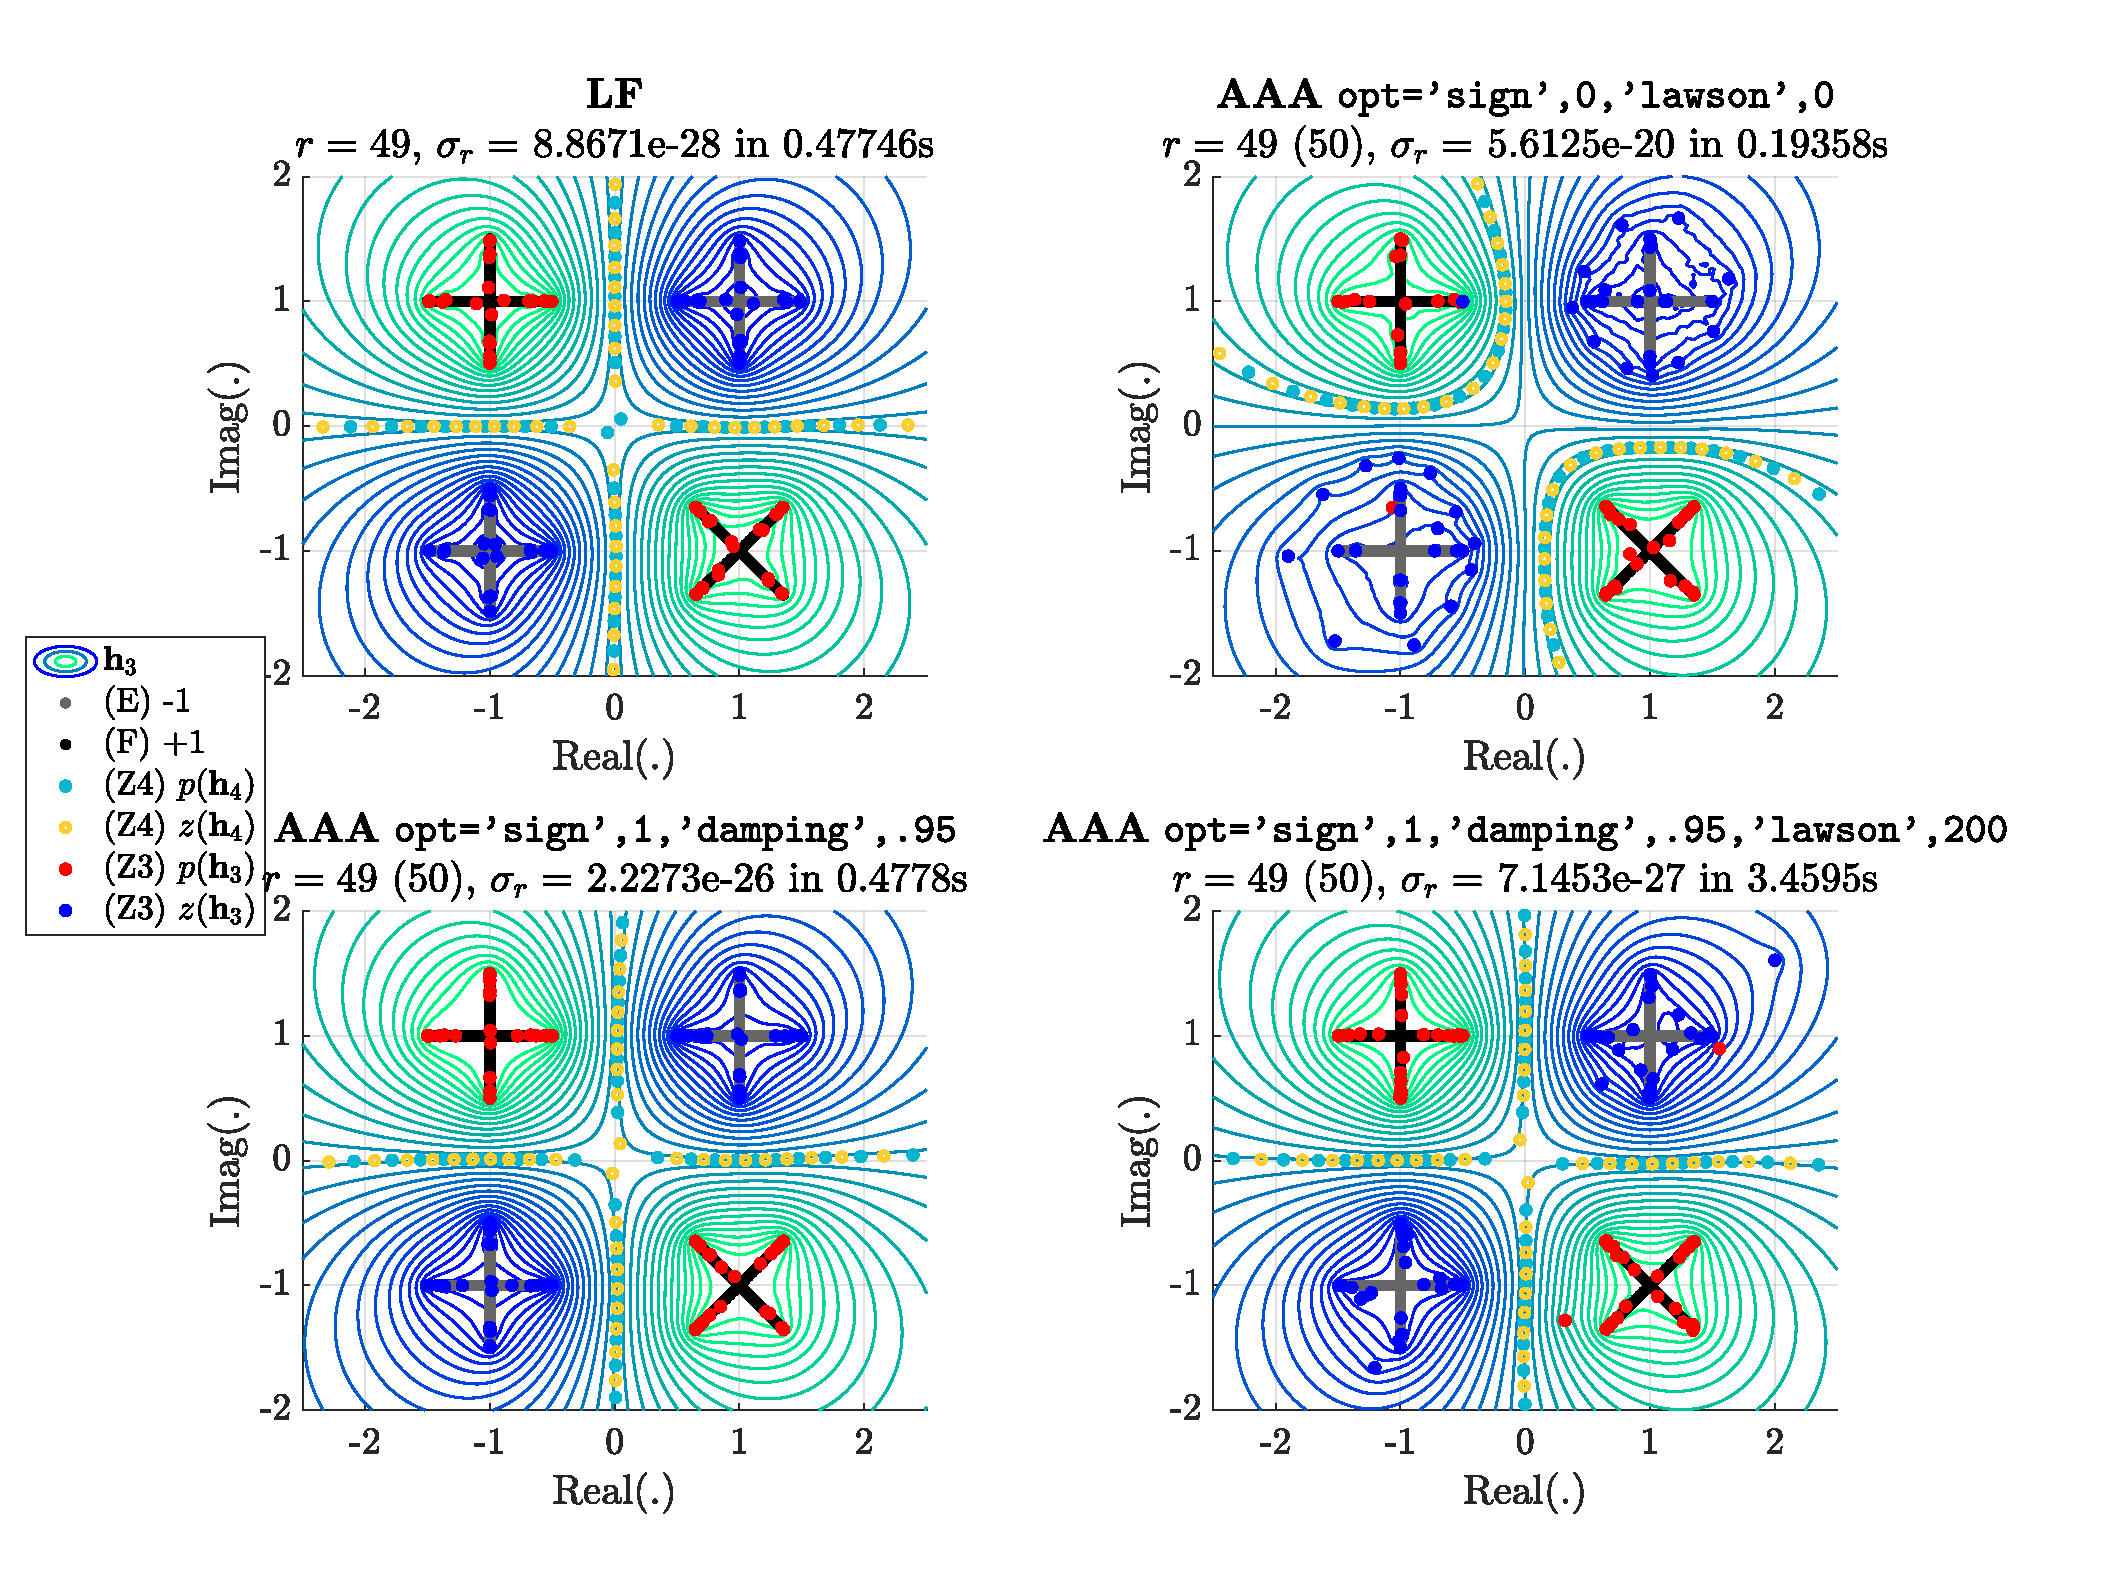
\includegraphics[width=.75\textwidth,align=c]{figures/all/cas_2c_r1e-14.pdf}
    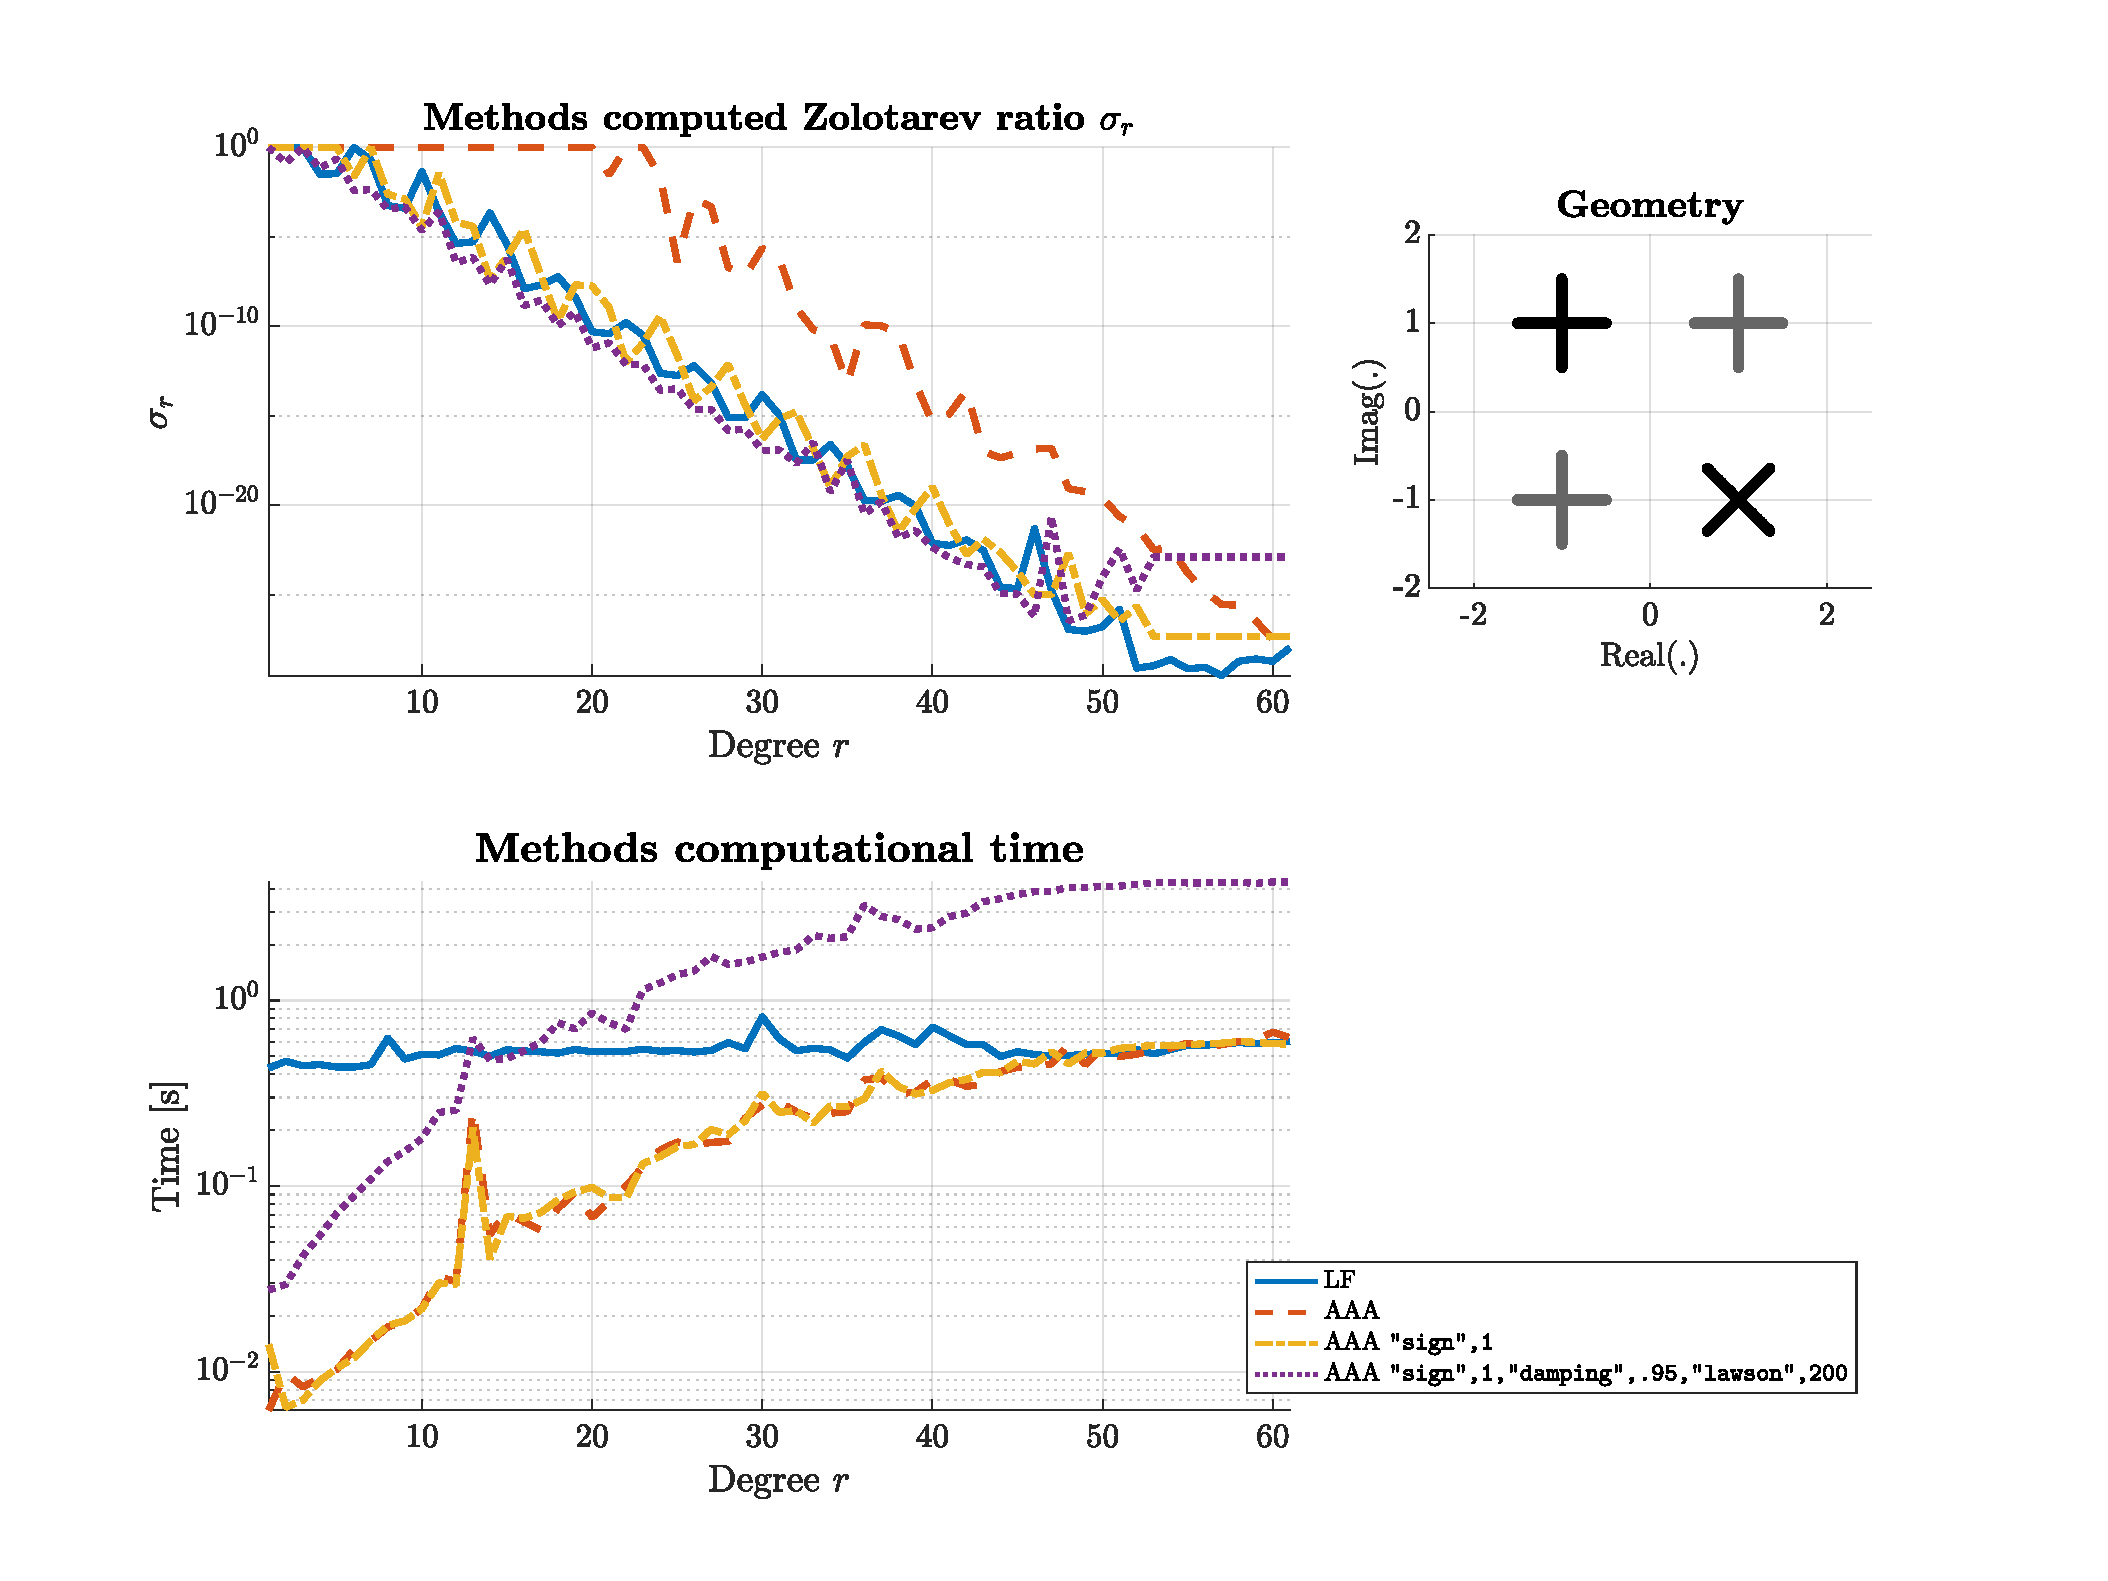
\includegraphics[width=.75\textwidth,align=c]{figures/time_accuracy/cas_2c_zol_time.pdf}
    \caption{Case \texttt{'2c'}. Top: same description as \cref{fig:intro:1a}. Bottom: same description as \cref{fig:intro:1a_time}.}
    \label{fig:2c}
\end{figure}

%%%%%%%%%%%%
\newpage
\subsection{Case \texttt{'2d'}}

This non-symmetric case illustrates a configuration where LF outperforms AAA, AAA with sign in accuracy (see lower frame in \cref{fig:2d}). In addition, the LF also provides better results than AAA with the sign and Lawson options when high accuracy is sought. 

\begin{figure}[H]
    \centering
    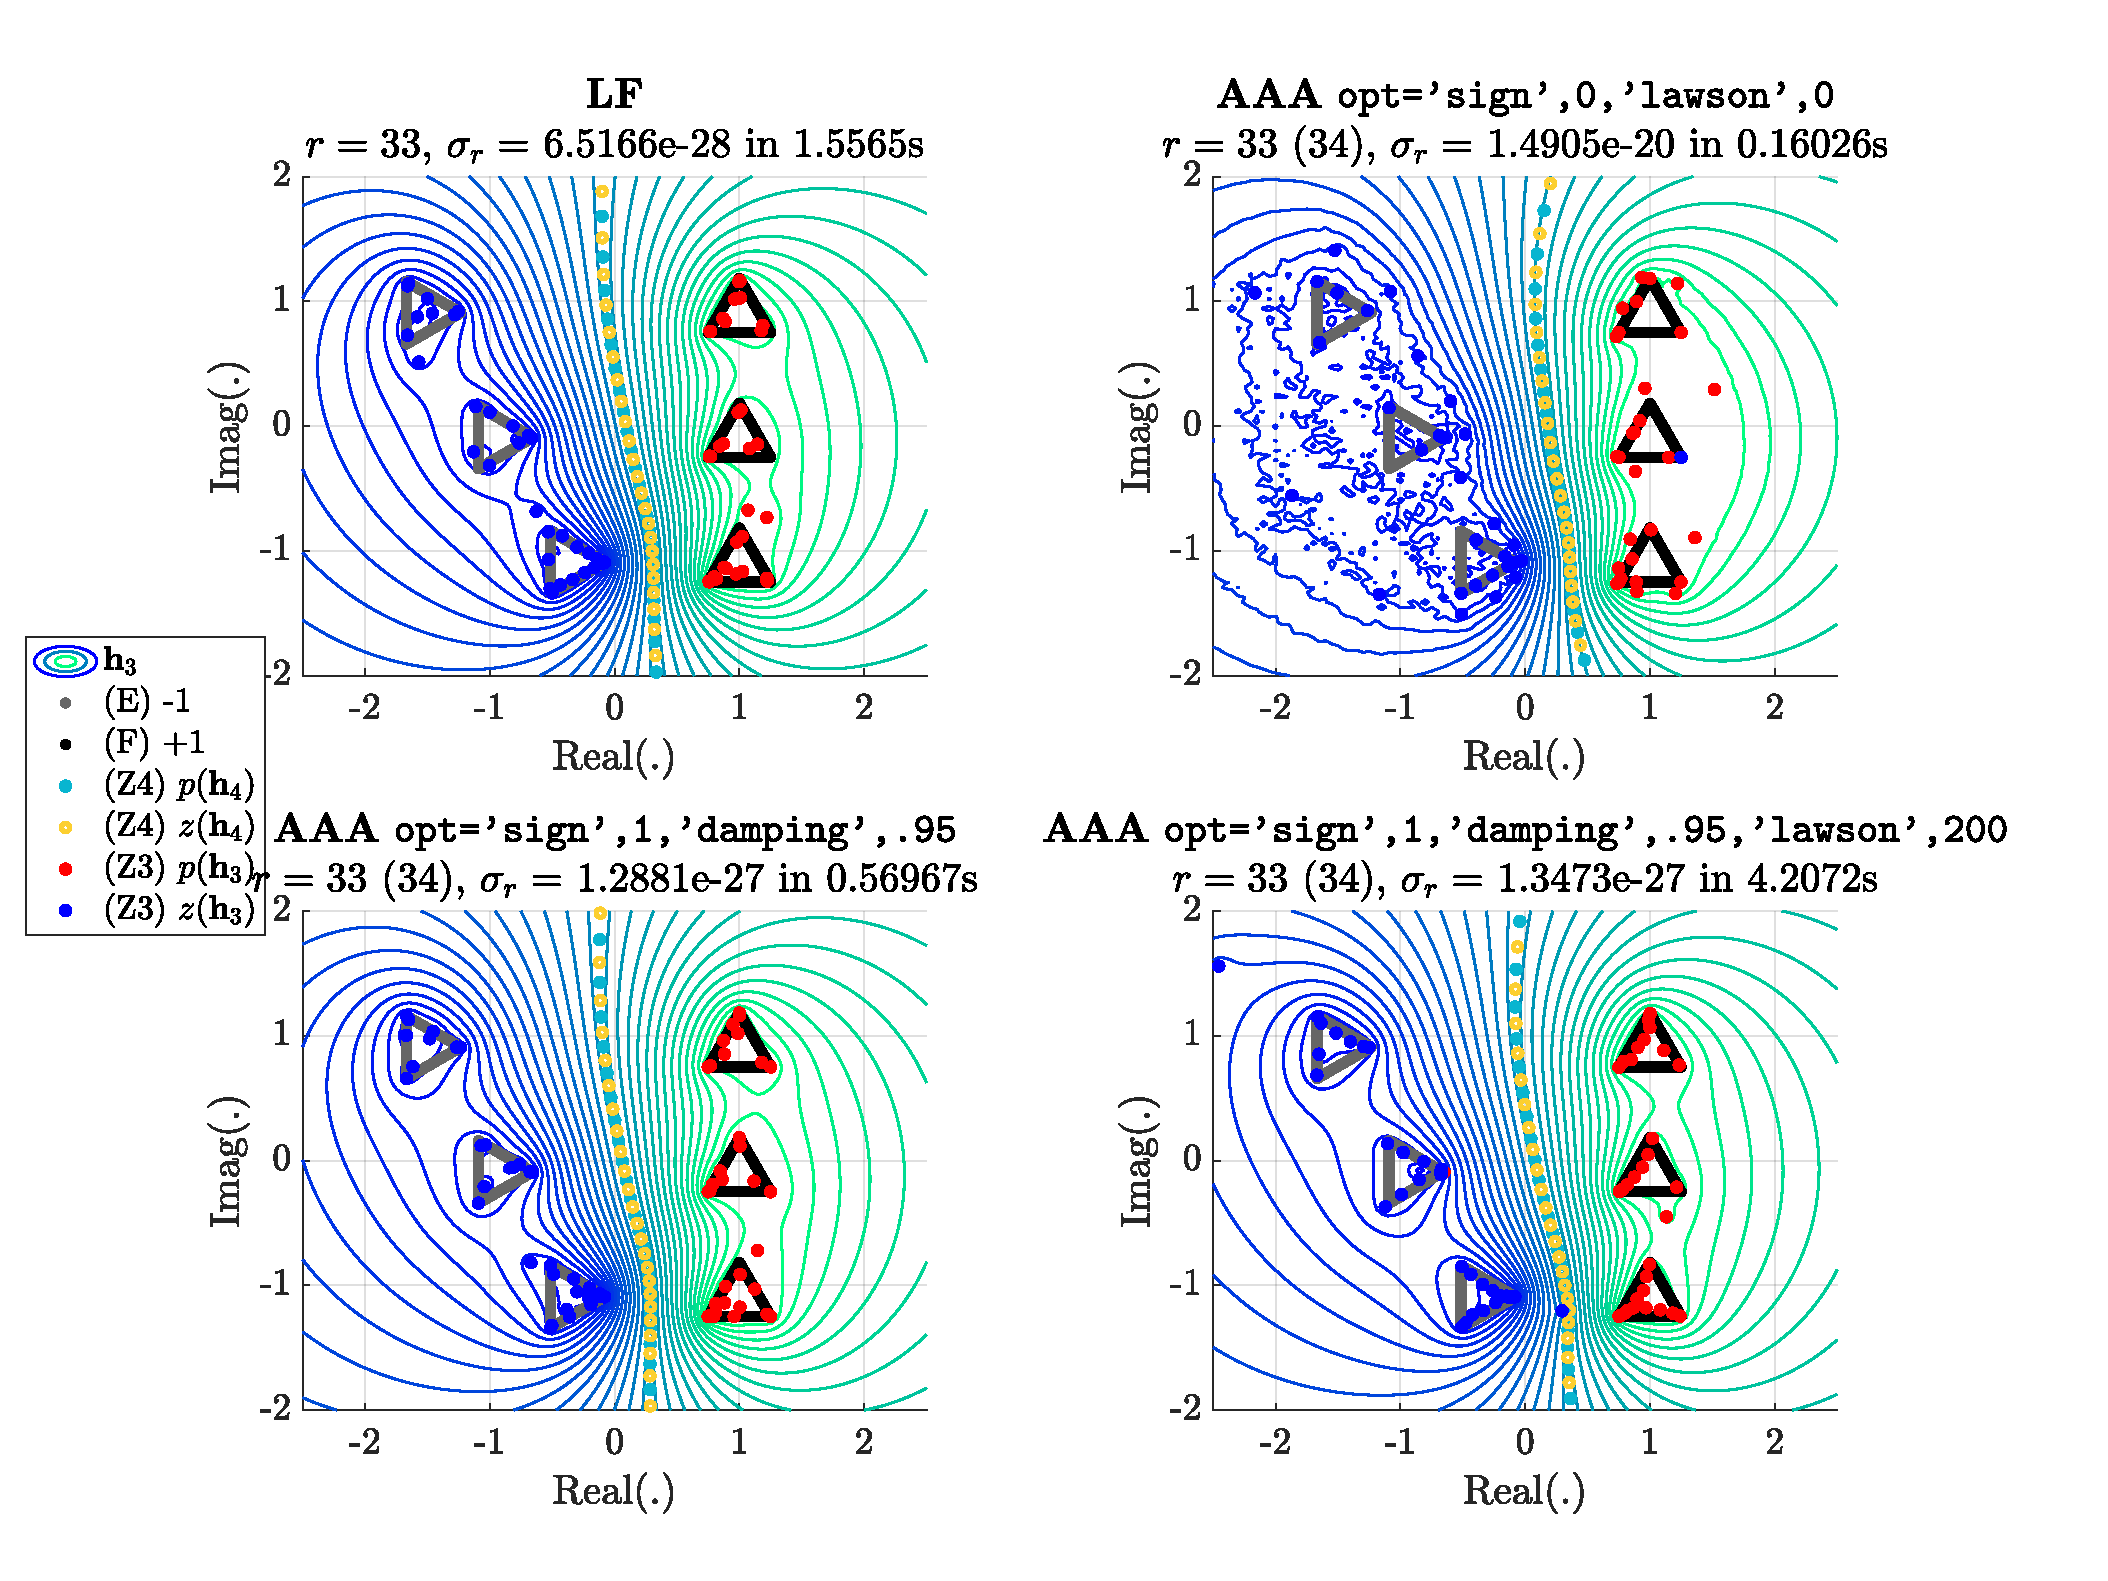
\includegraphics[width=.75\textwidth,align=c]{figures/all/cas_2d_r1e-14.pdf}
    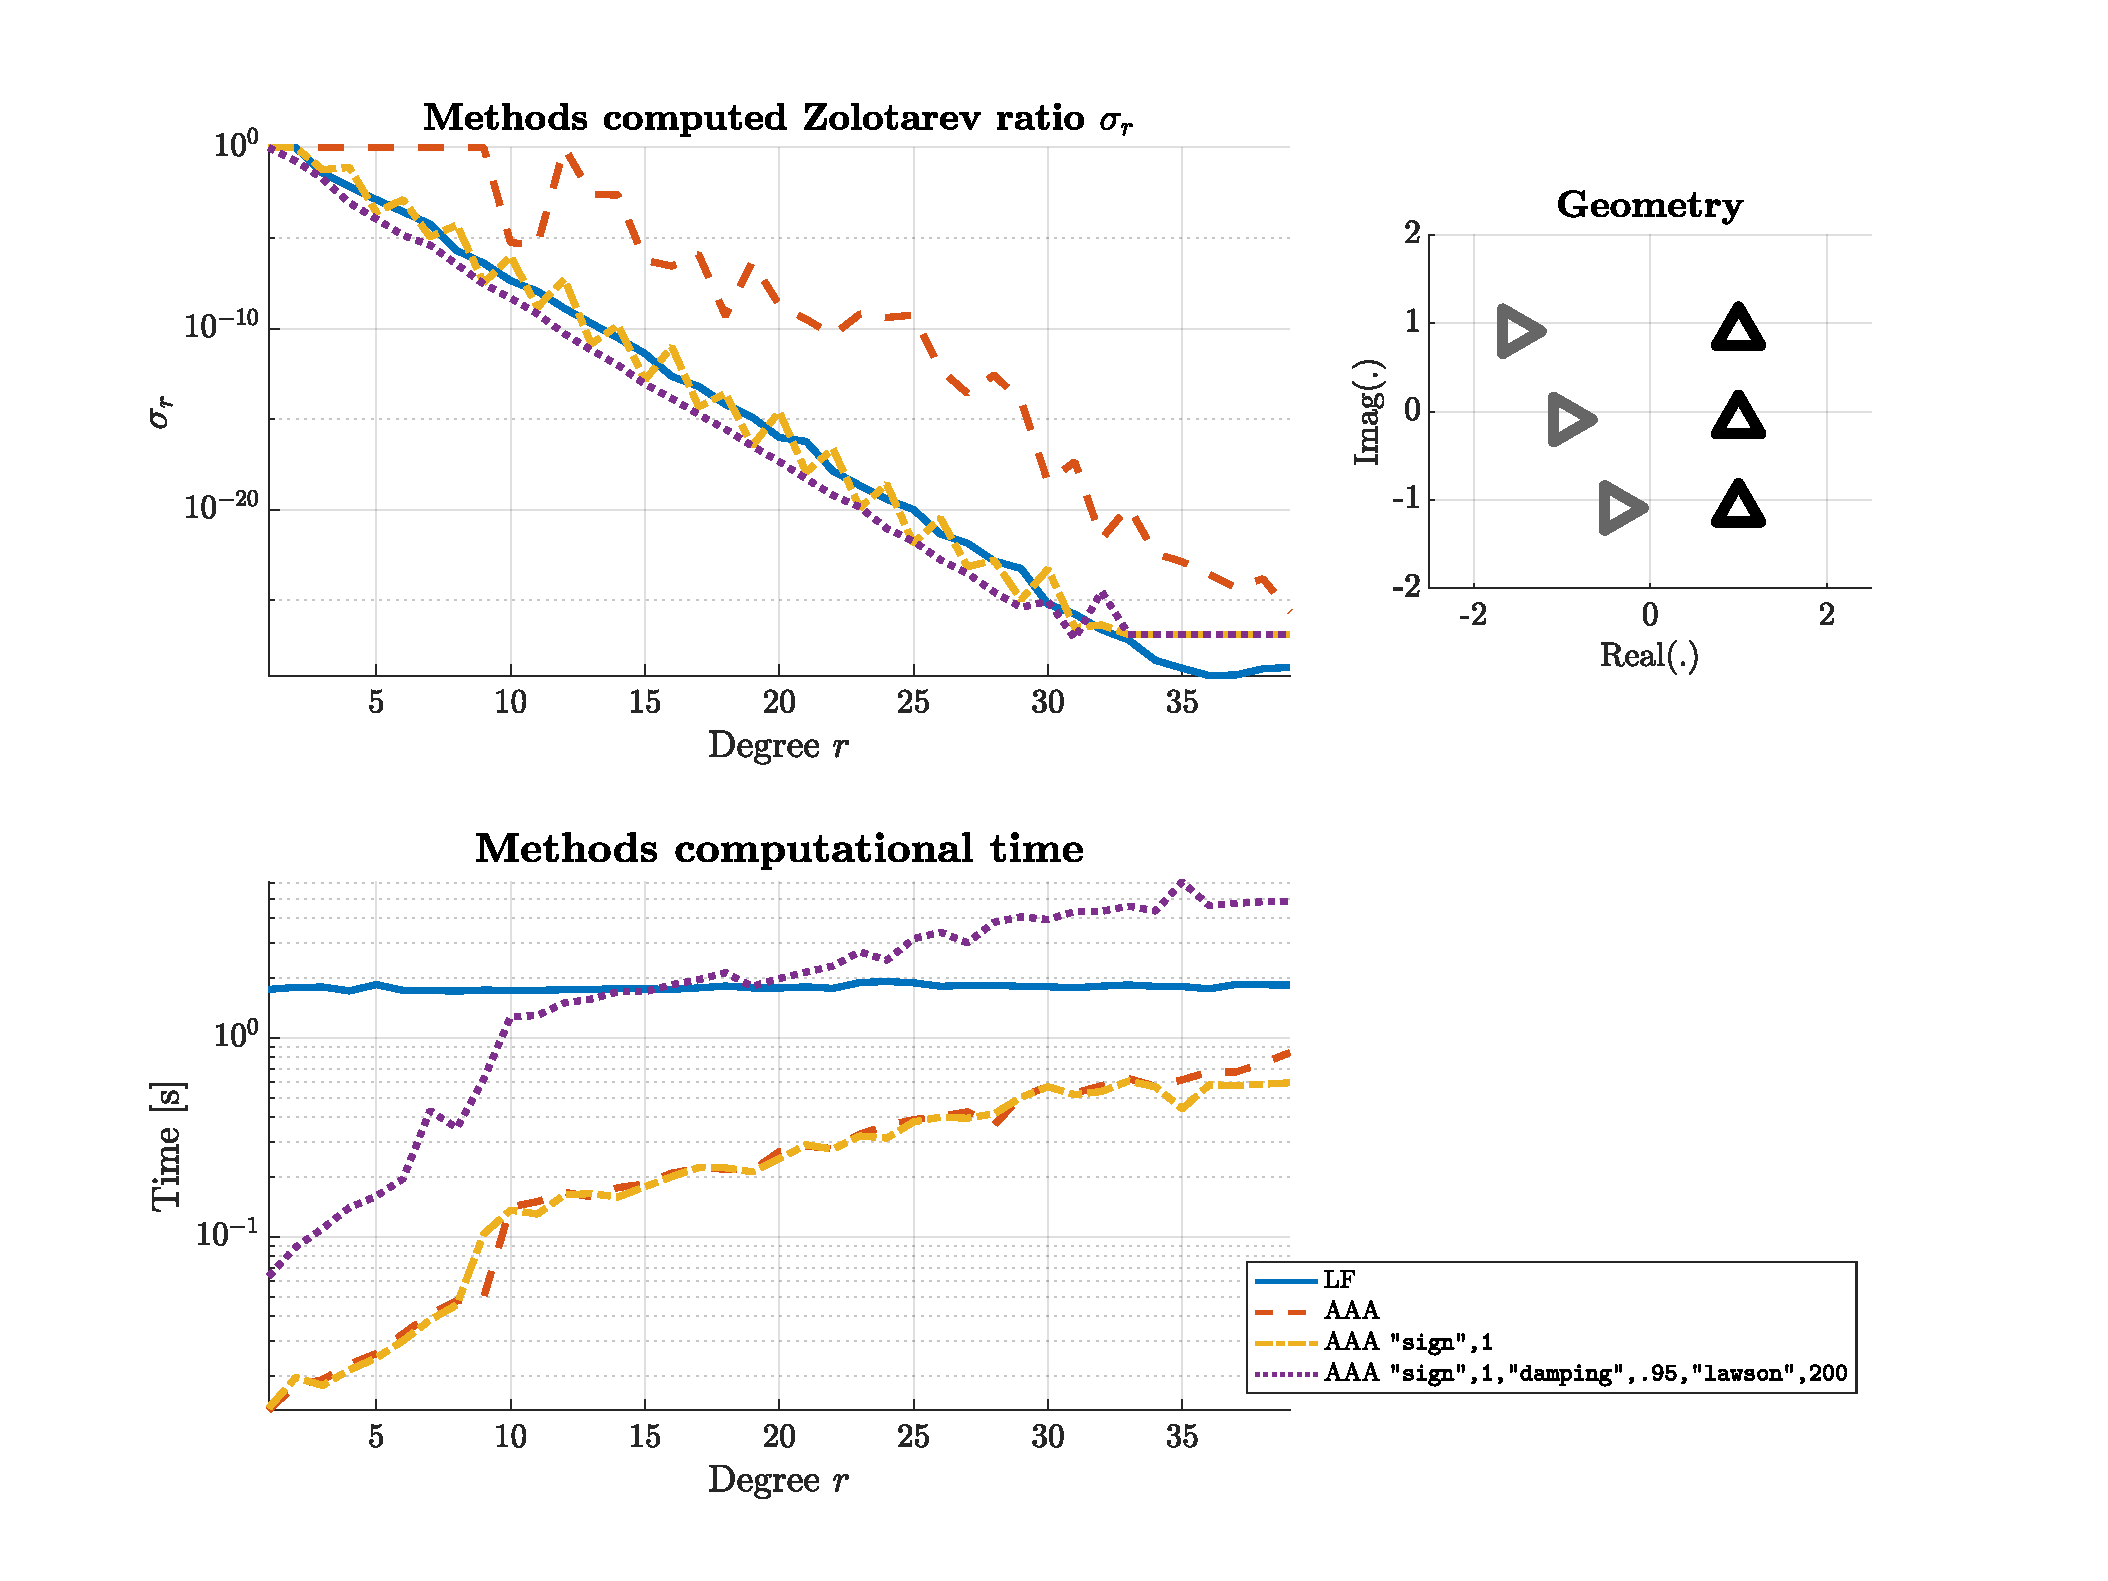
\includegraphics[width=.75\textwidth,align=c]{figures/time_accuracy/cas_2d_zol_time.pdf}
    \caption{Case \texttt{'2d'}. Top: same description as \cref{fig:intro:1a}. Bottom: same description as \cref{fig:intro:1a_time}.}
    \label{fig:2d}
\end{figure}

%%%%%%%%%%%%
\newpage
\subsection{Case \texttt{'3a'}, \texttt{'3b'}, \texttt{'3c'}, \texttt{'3d'}}

Now we consider four configurations for which the sets are not disjoint, but $E$ is inside $F$. The results are reported in \cref{fig:3a,fig:3b}. In all these settings, the AAA configuration performs better than LF (except in computational time). It appears in all these cases that the LF needs a very high rational order  to achieve a good approximation, while the AAA sign and the AAA sign Lawson perform well already with low approximation orders. This aspect is not well understood yet, but certainly shows the usefulness of the Lawson and sign features in certain cases.

\begin{figure}[H]
    \centering
    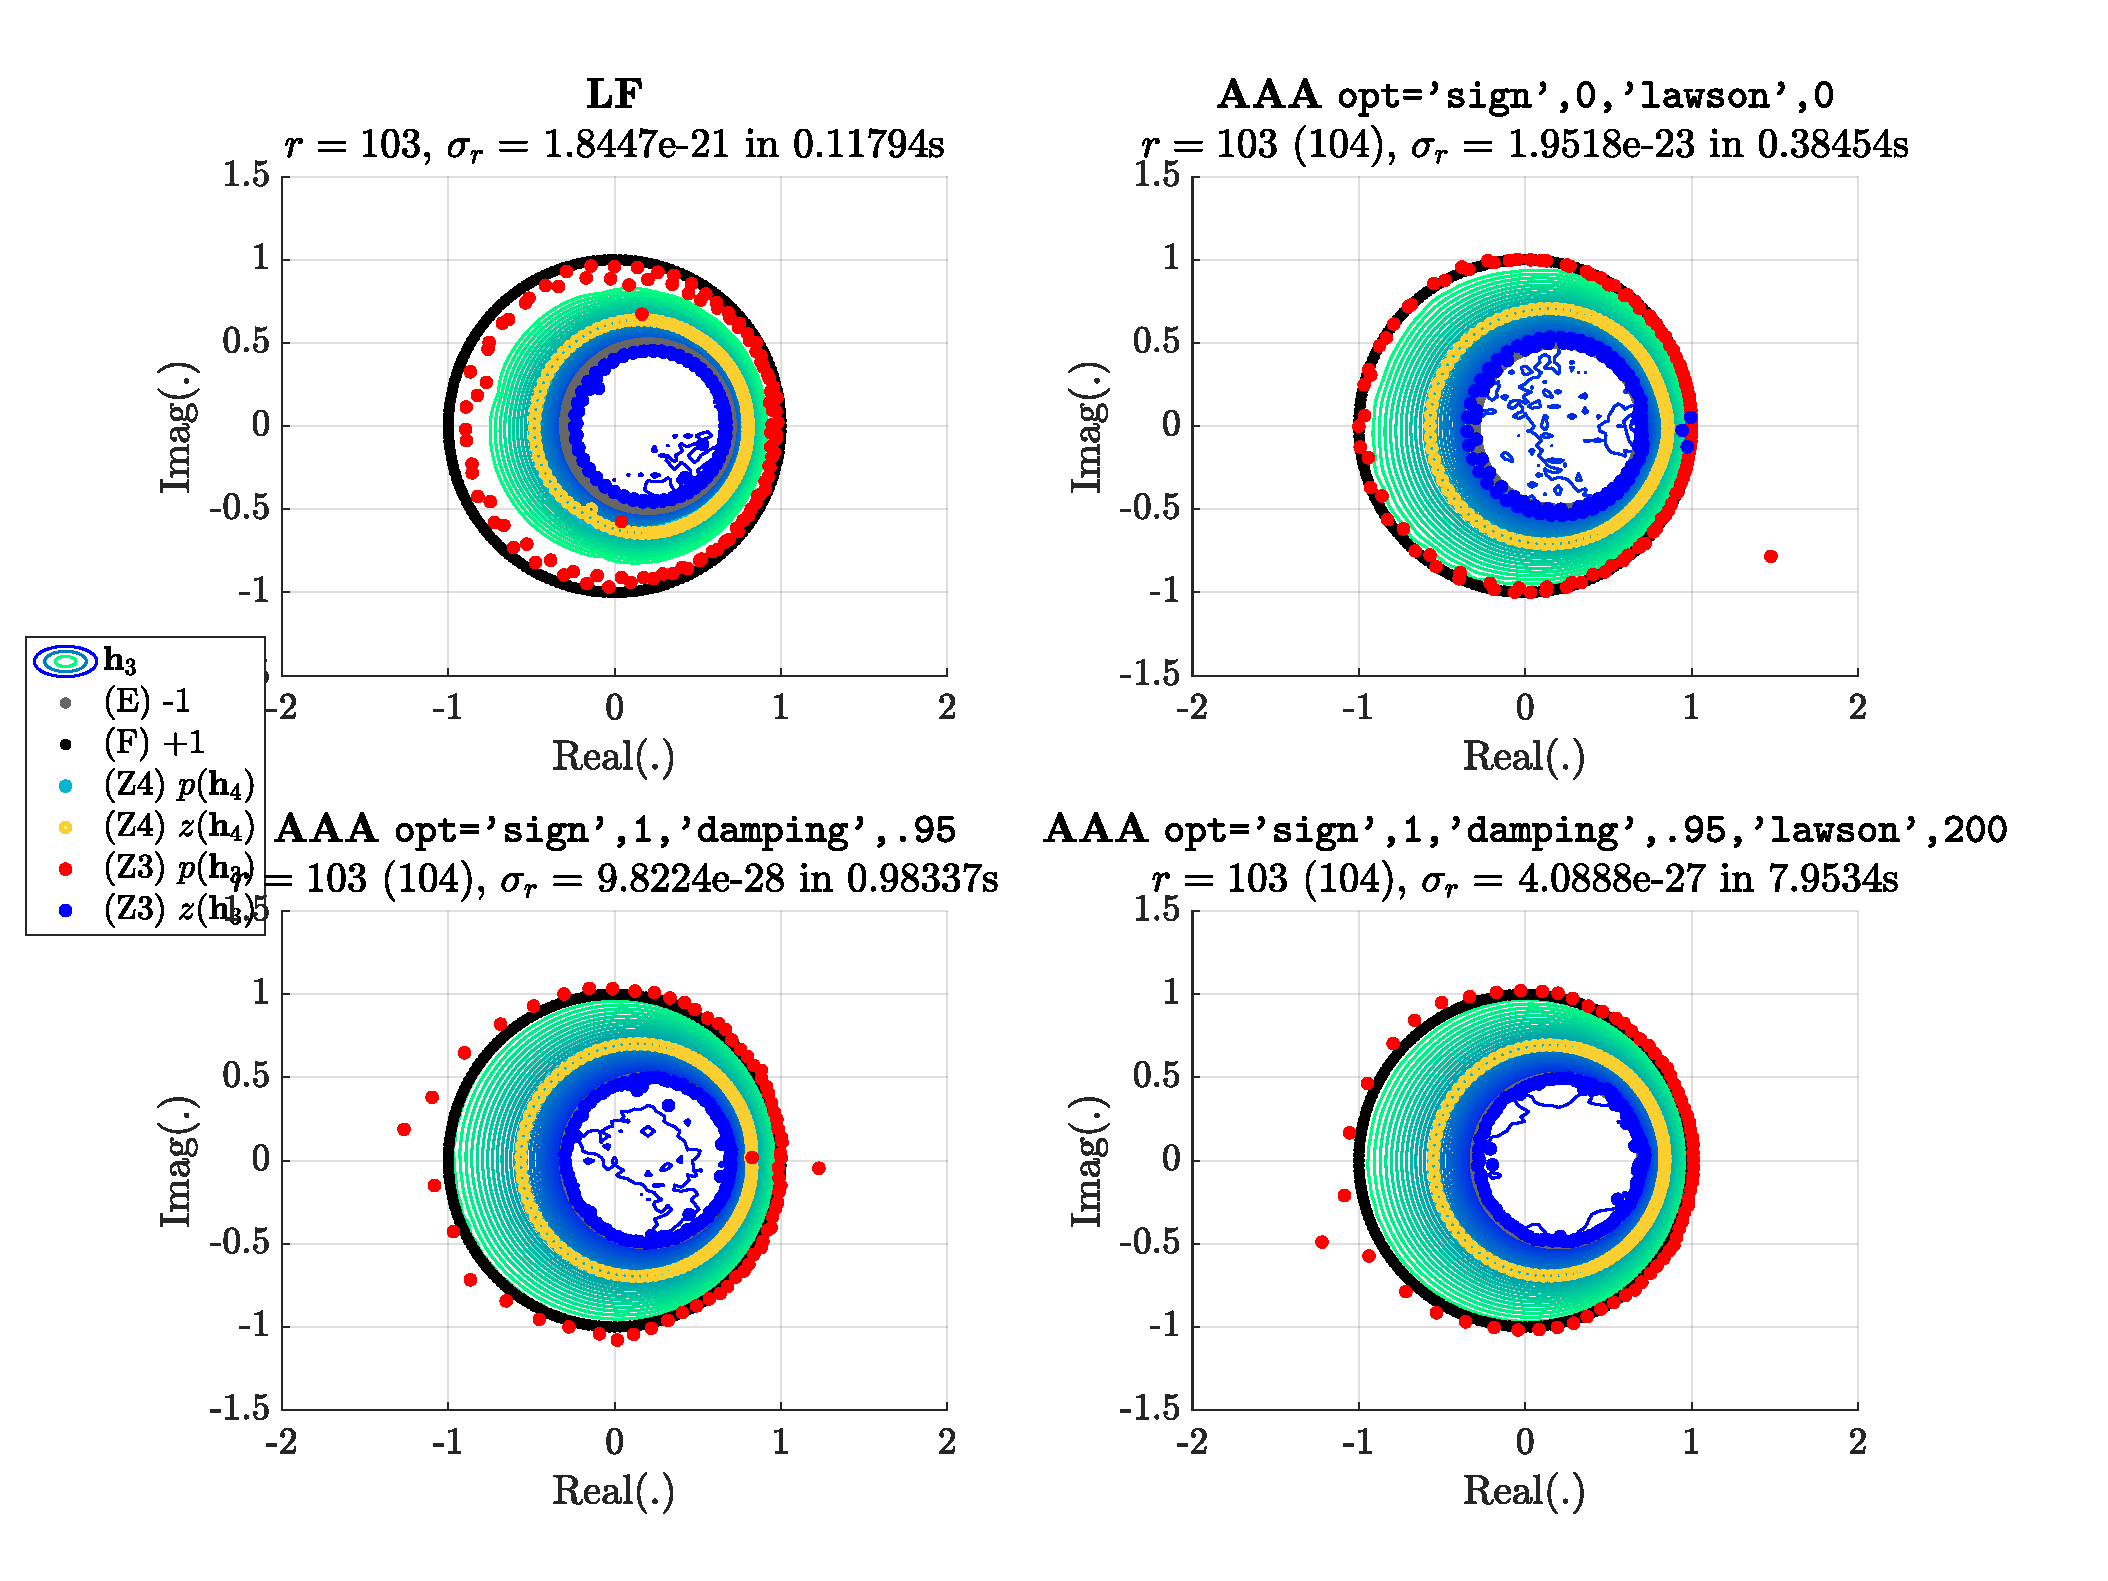
\includegraphics[width=.45\textwidth,align=c]{figures/all/cas_3a_r1e-14.pdf}
    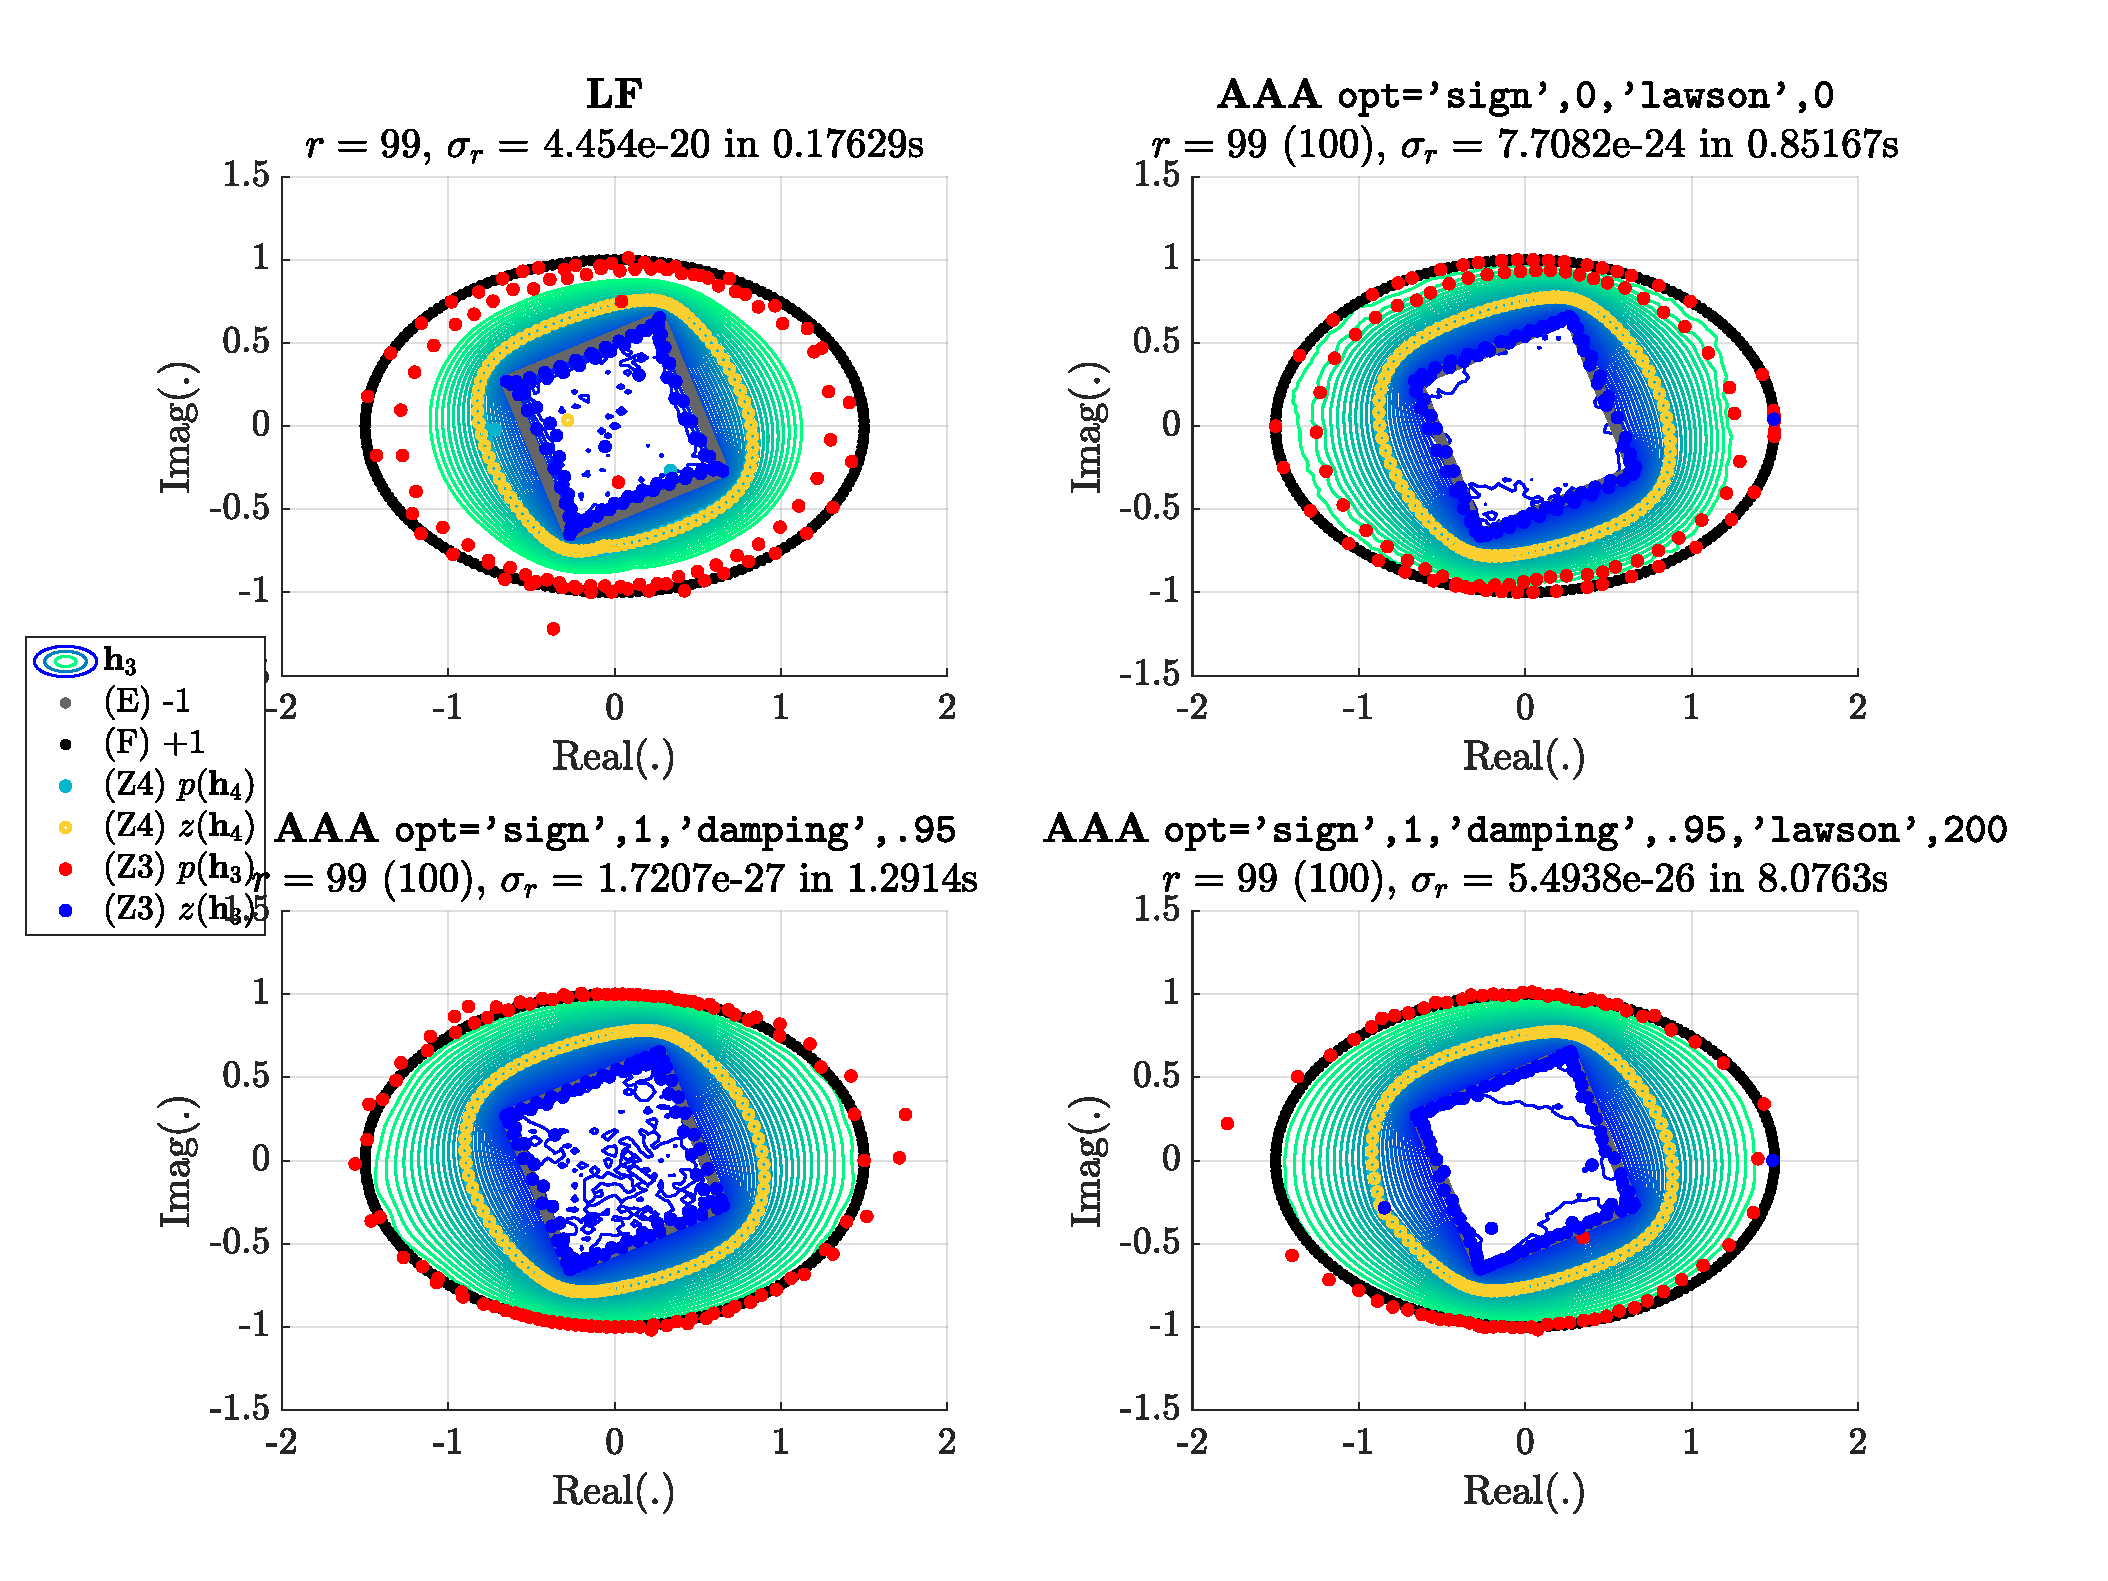
\includegraphics[width=.45\textwidth,align=c]{figures/all/cas_3b_r1e-14.pdf}\\
    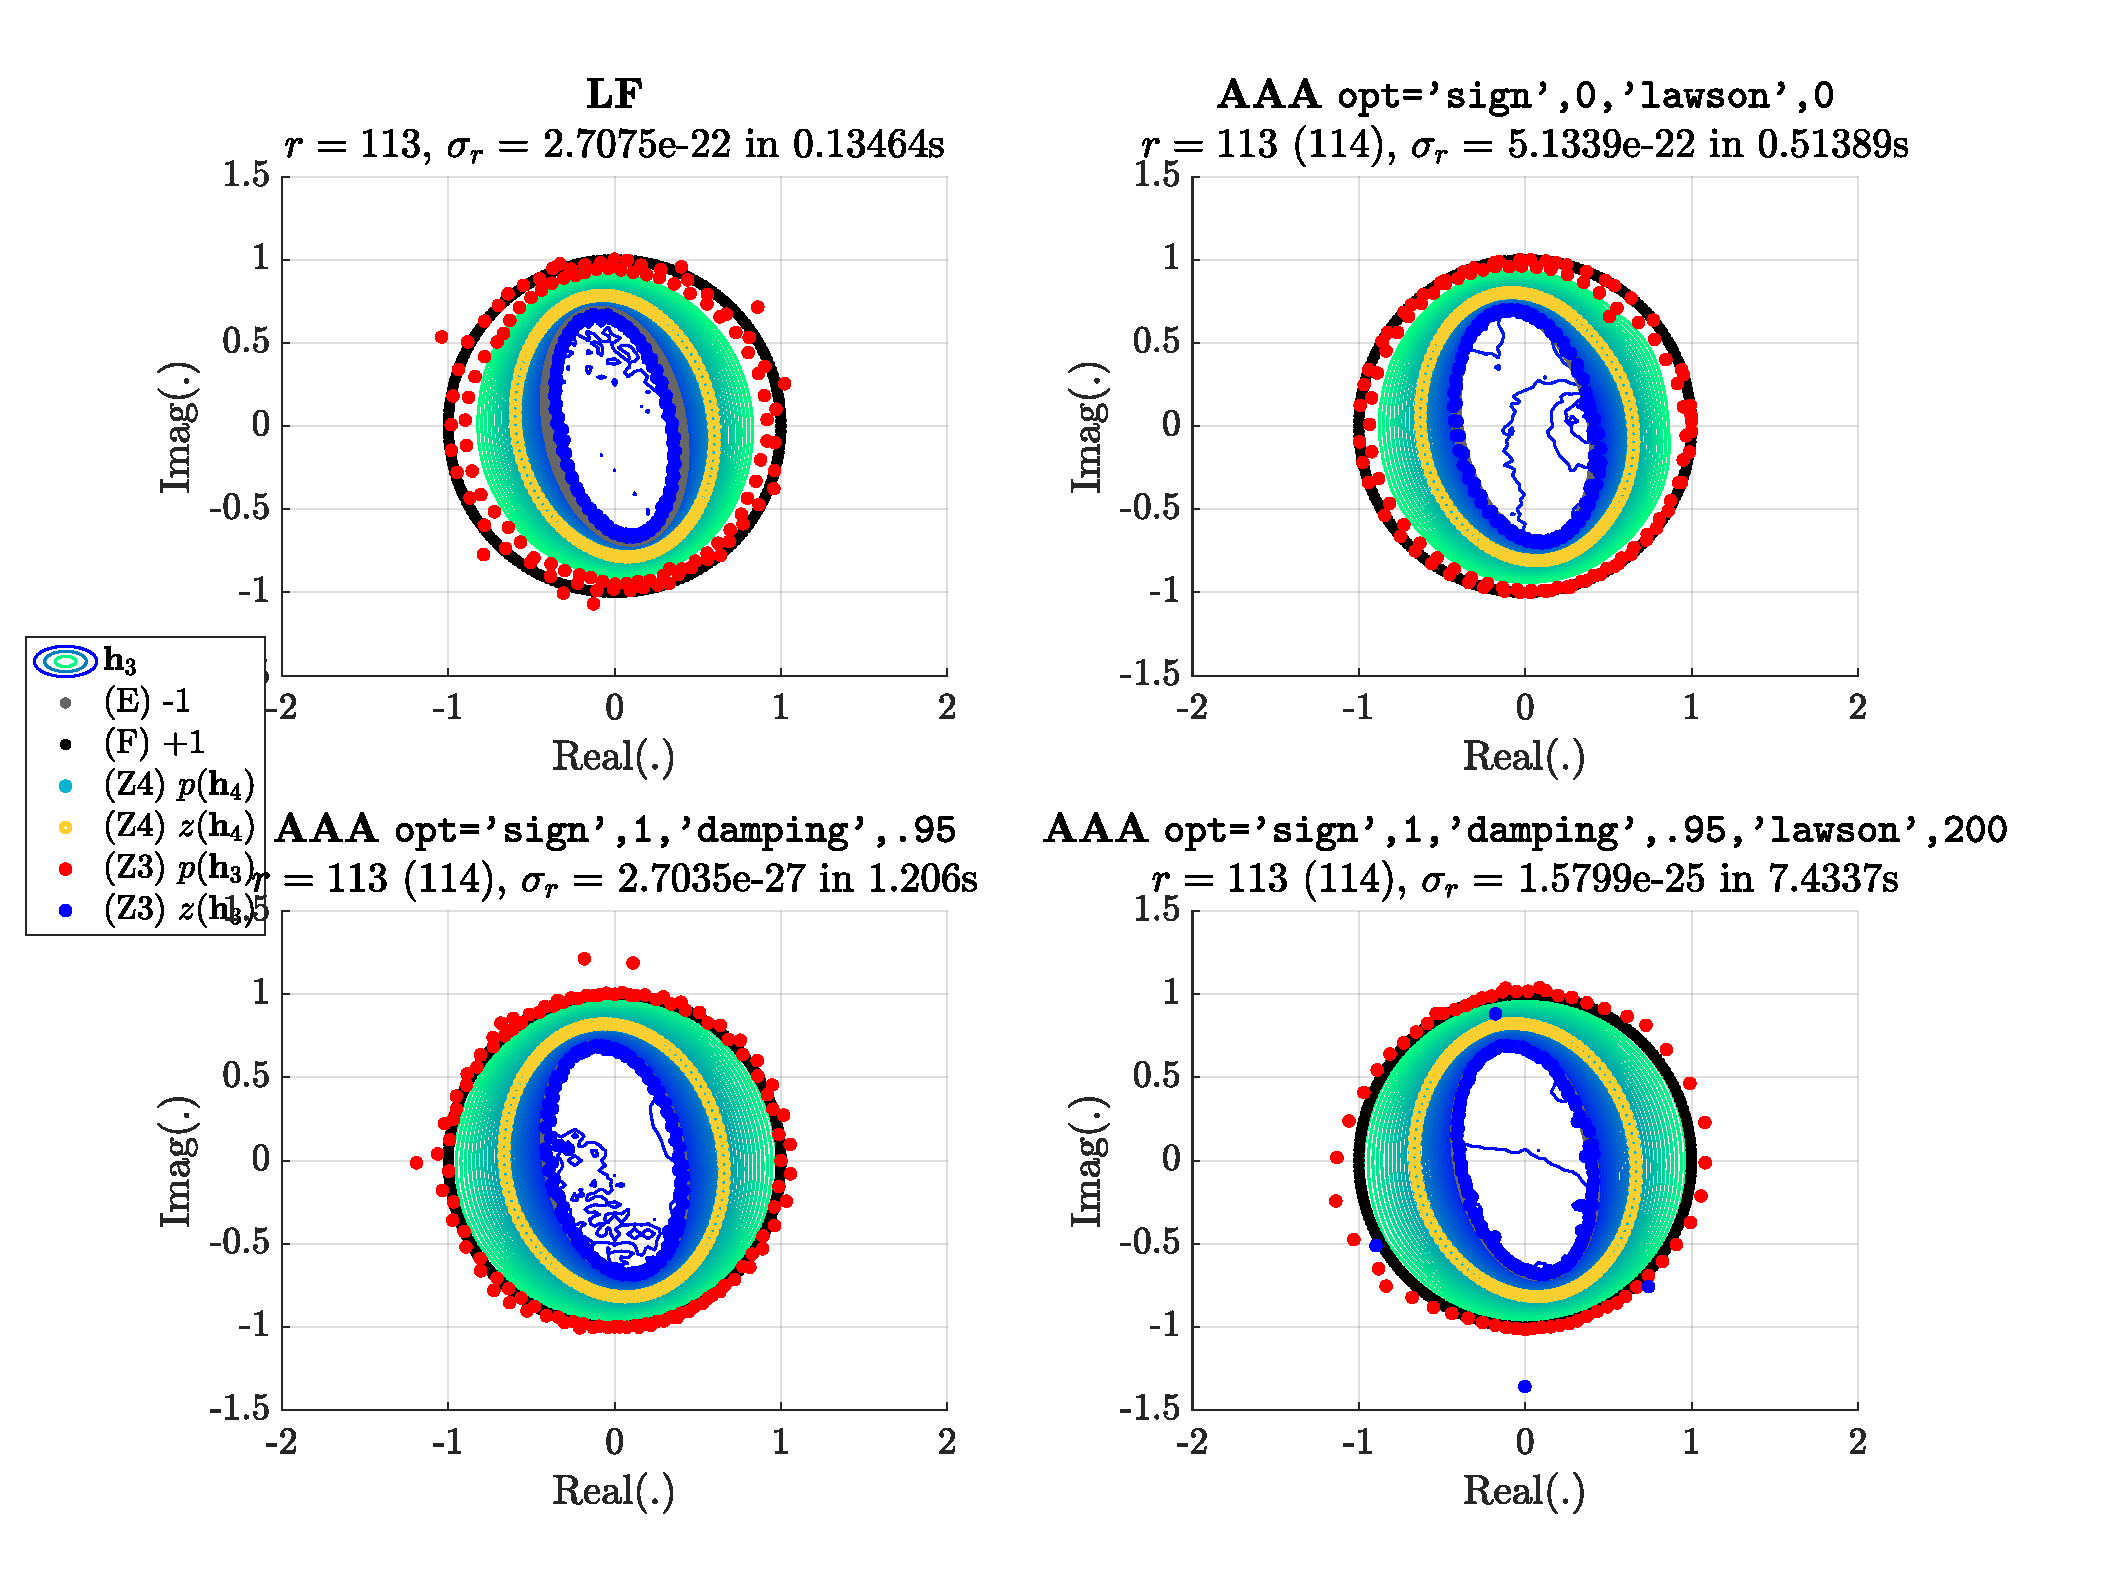
\includegraphics[width=.45\textwidth,align=c]{figures/all/cas_3c_r1e-14.pdf}
    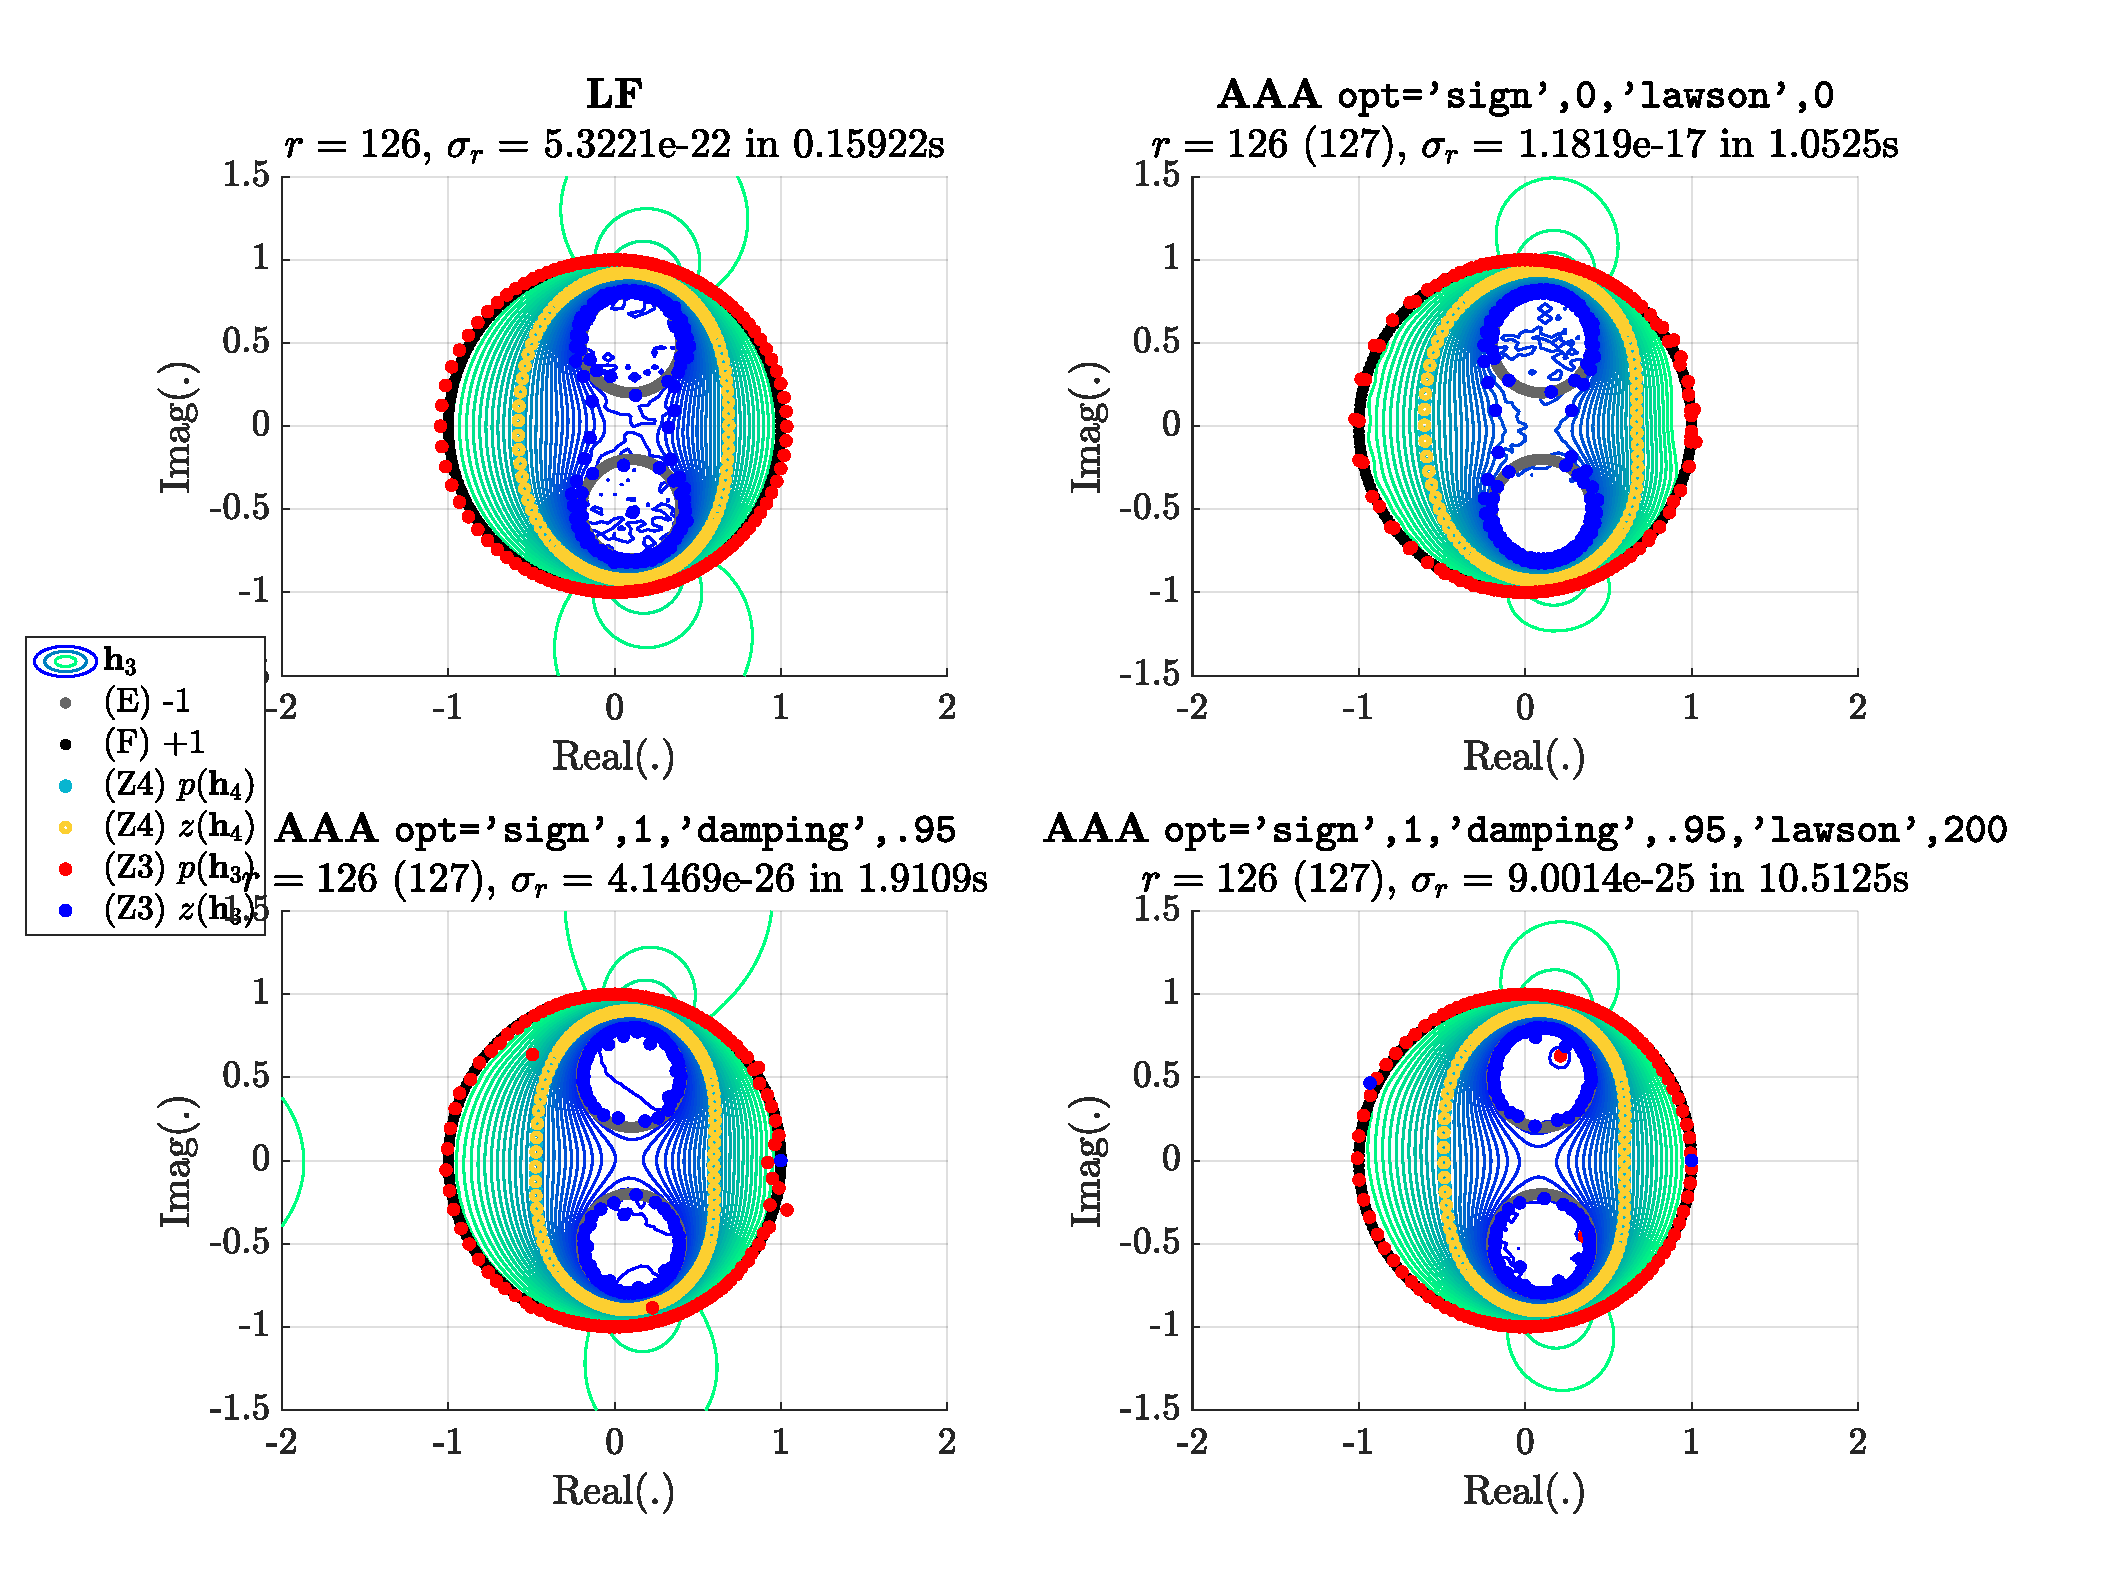
\includegraphics[width=.45\textwidth,align=c]{figures/all/cas_3d_r1e-14.pdf}
    \caption{Case \texttt{'3a,b,c,d'}. Same description as \cref{fig:intro:1a}.}
    \label{fig:3a}
\end{figure}

\begin{figure}[H]
    \centering
    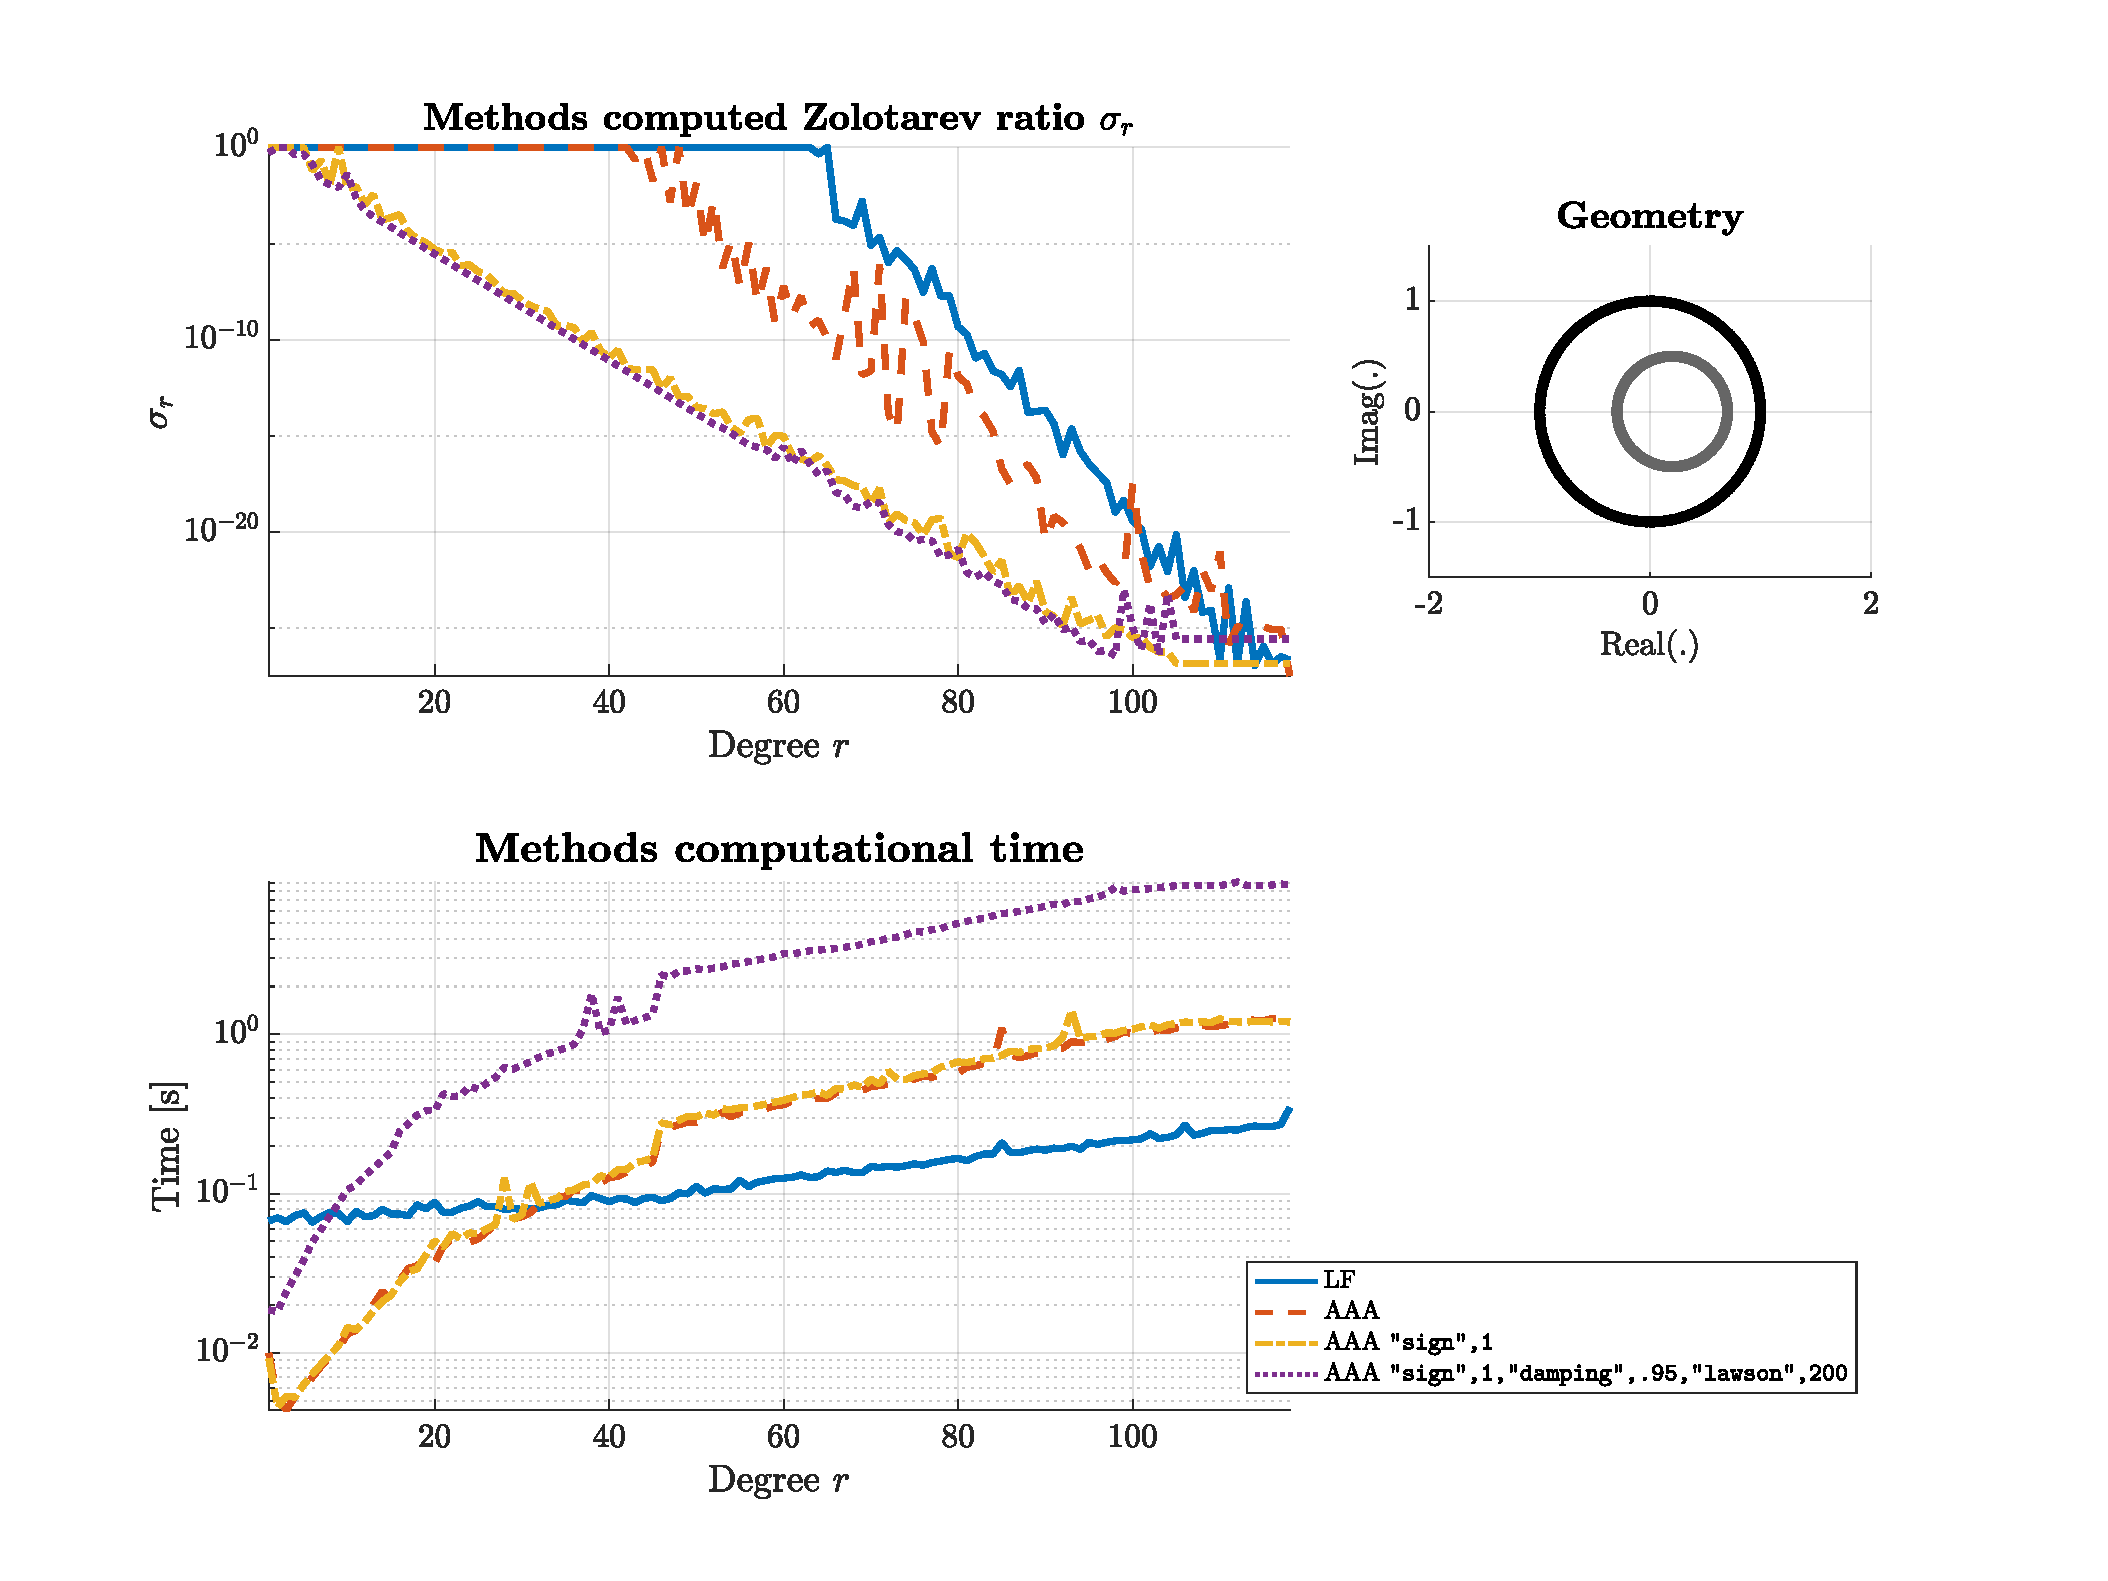
\includegraphics[width=.45\textwidth,align=c]{figures/time_accuracy/cas_3a_zol_time.pdf}
    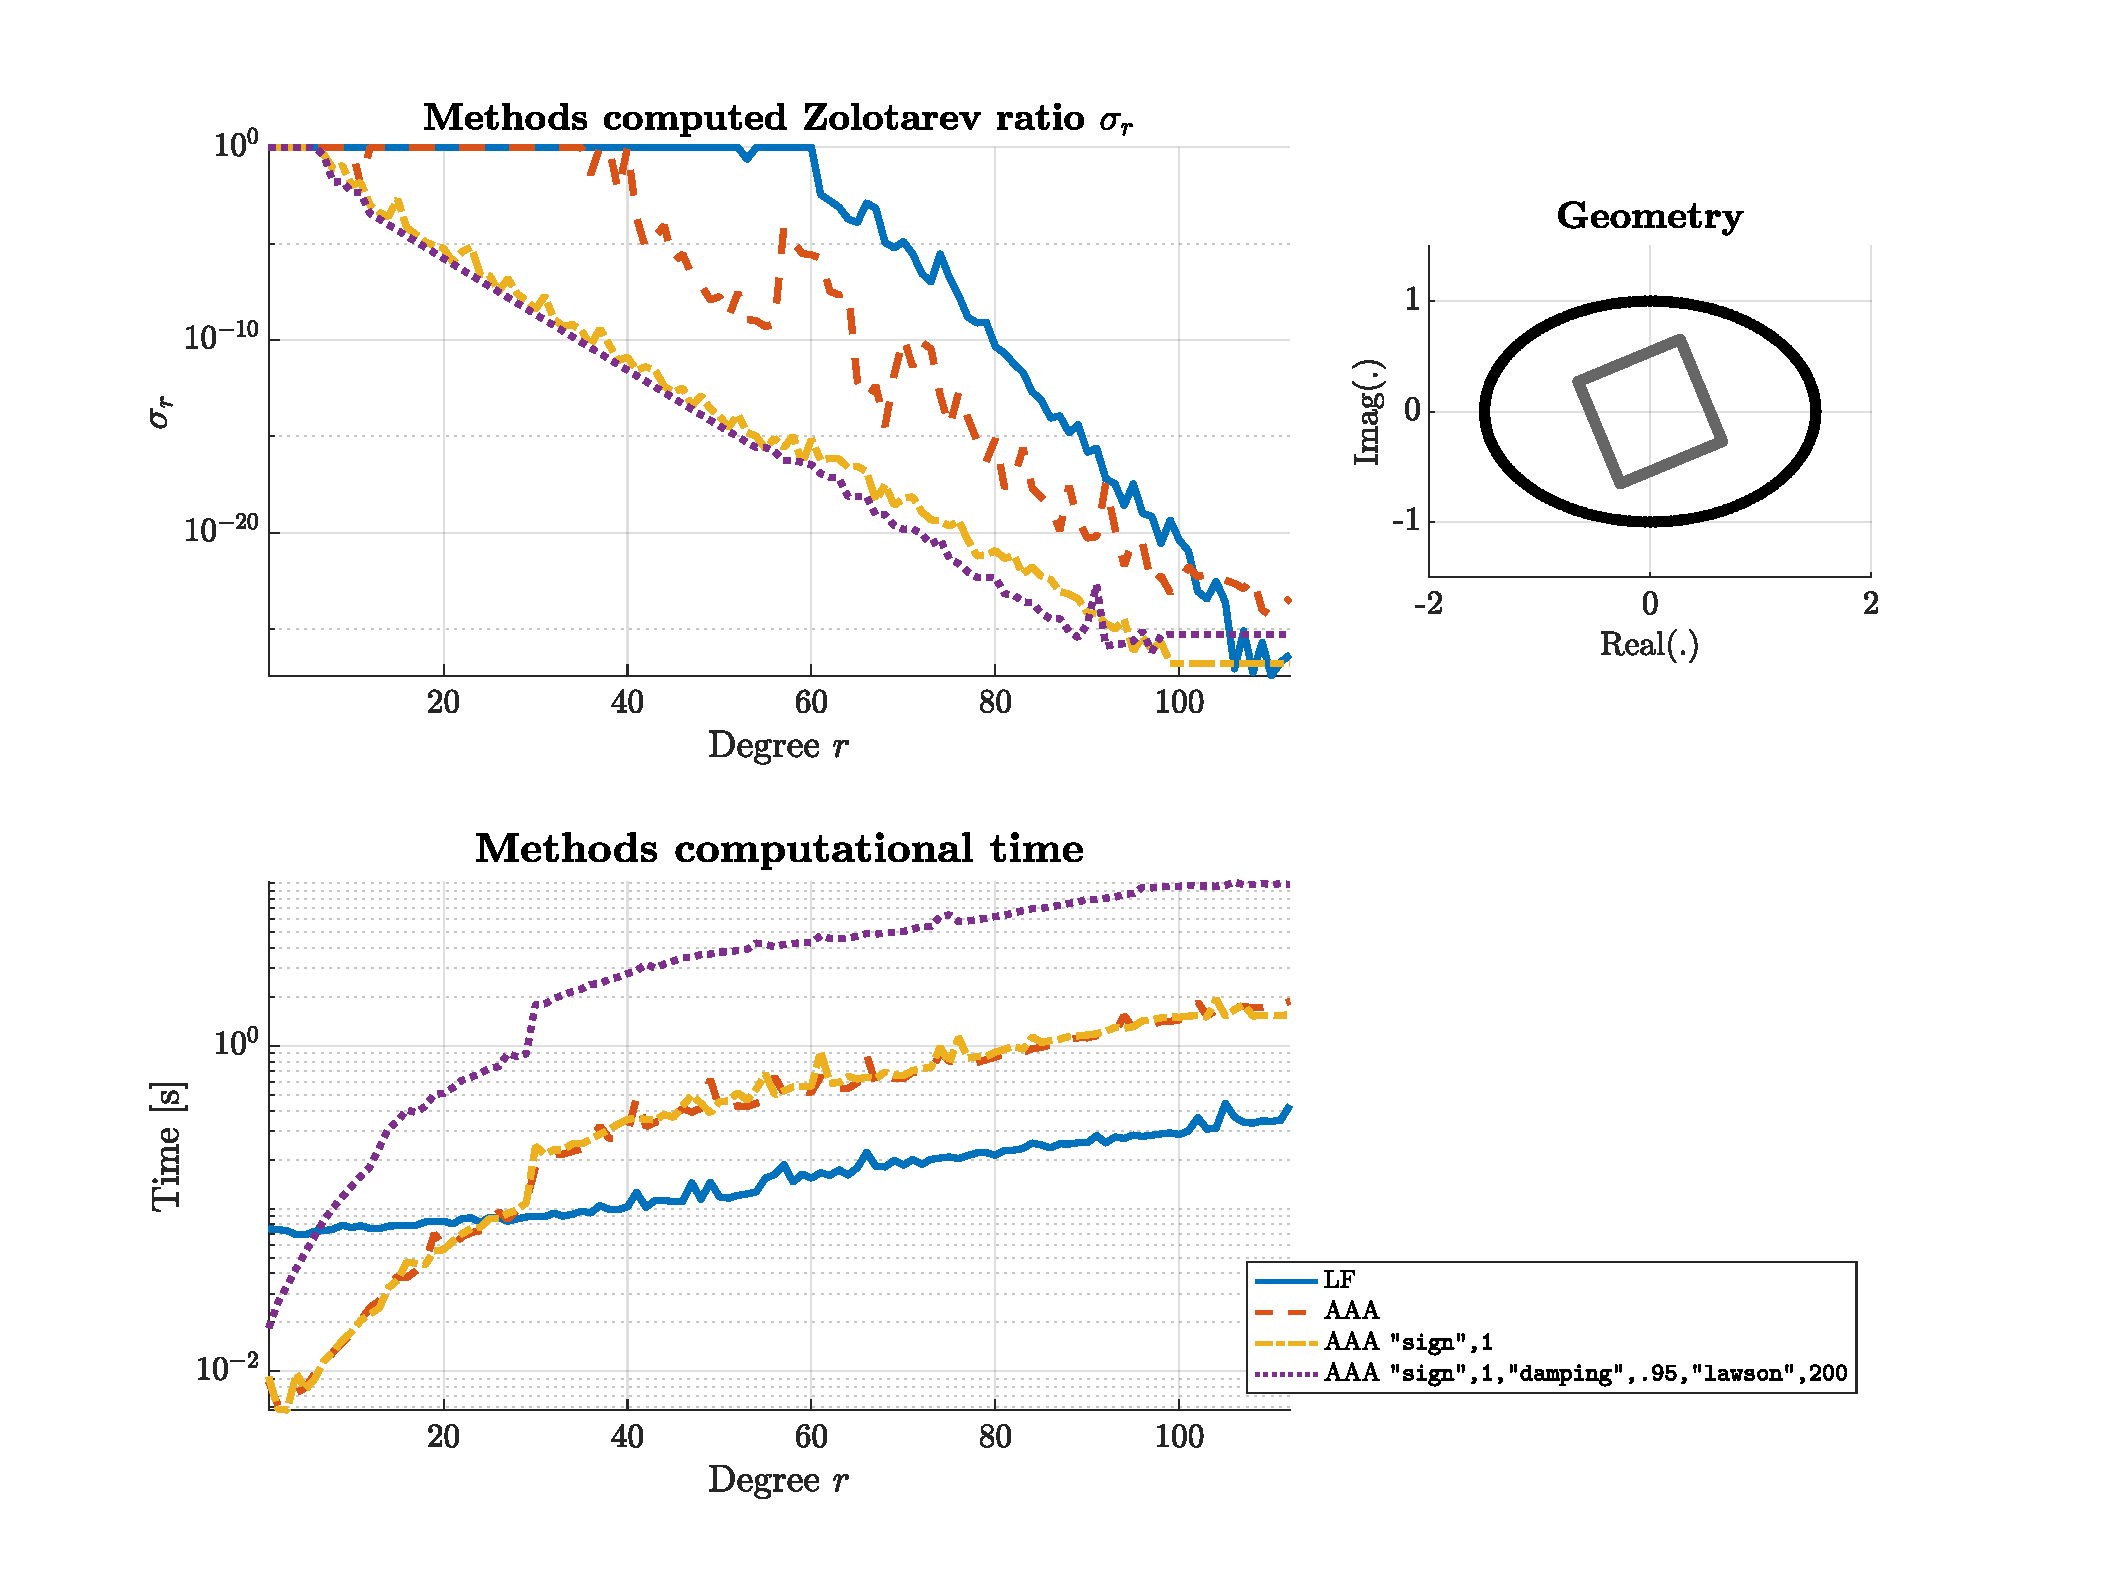
\includegraphics[width=.45\textwidth,align=c]{figures/time_accuracy/cas_3b_zol_time.pdf}
    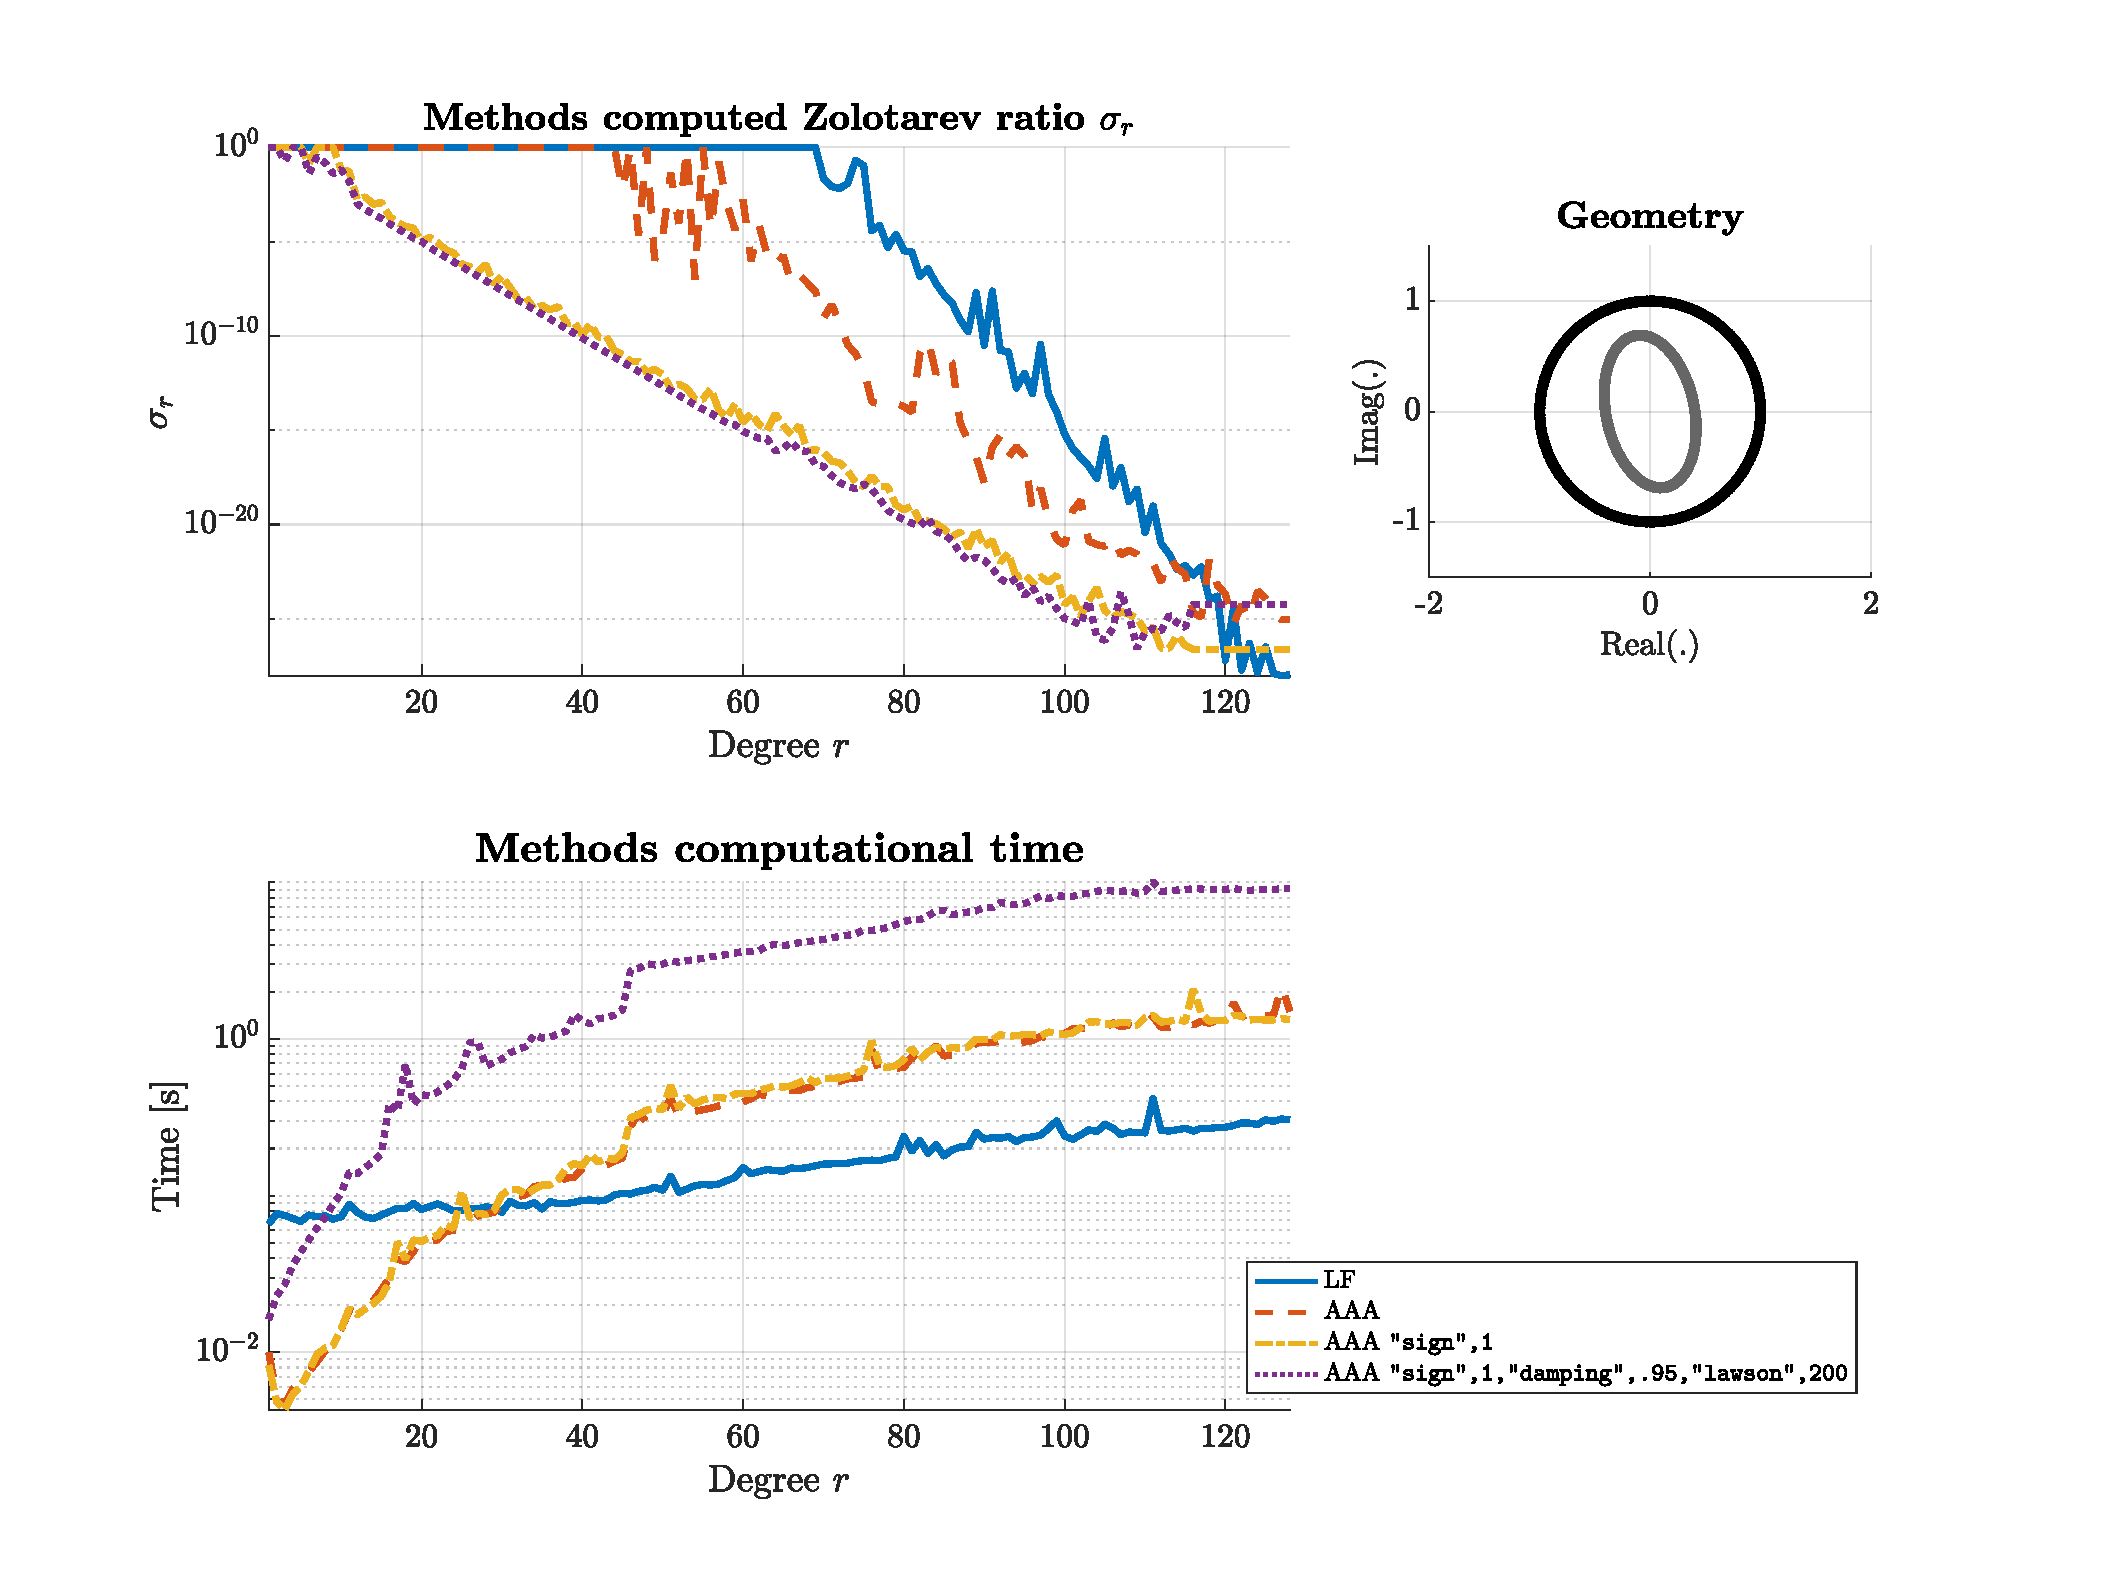
\includegraphics[width=.45\textwidth,align=c]{figures/time_accuracy/cas_3c_zol_time.pdf}
    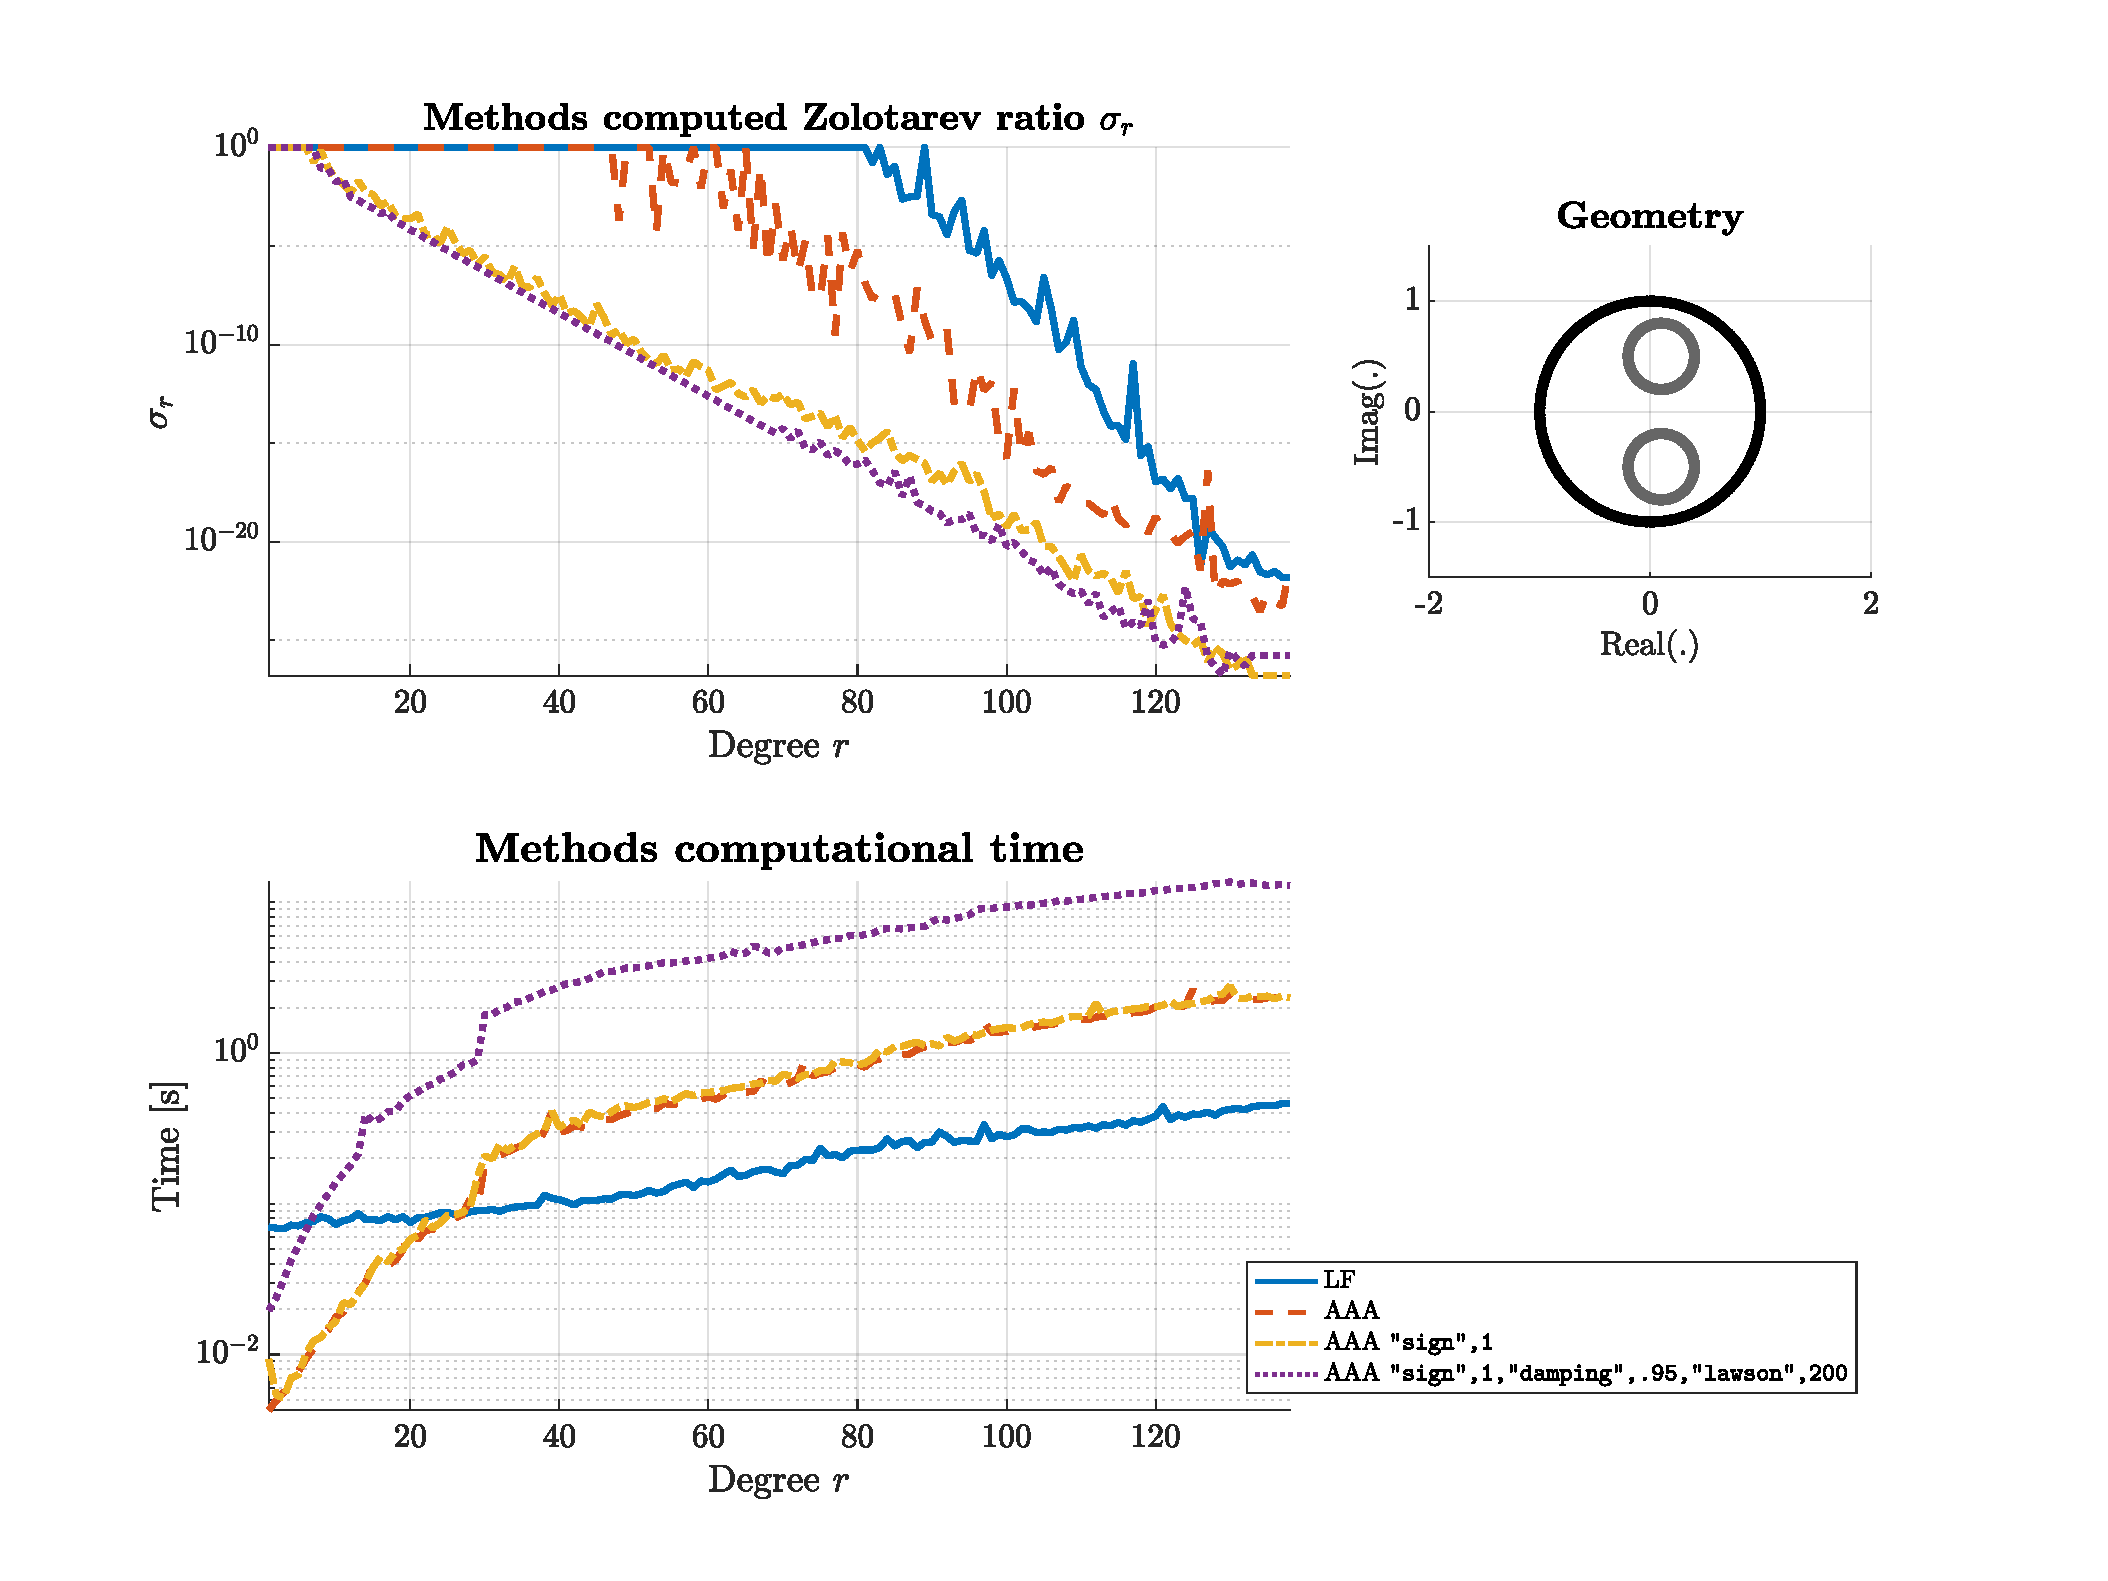
\includegraphics[width=.45\textwidth,align=c]{figures/time_accuracy/cas_3d_zol_time.pdf}
    \caption{Case \texttt{'3a,b,c,d'}. Same description as \cref{fig:intro:1a_time}.}
    \label{fig:3b}
\end{figure}


%%%%%%%%%%%%
\newpage
\subsection{Case \texttt{'7'}}

The two-rectangle case shown in \cref{fig:7} illustrates the benefit of the LF with respect to AAA versions in terms of computational time. Again, the latter is perfectly flat and constant with almost the same accuracy. Moreover, in the configuration shown in the frame above, the approximation is even better with LF. Notice again the clean pole/zero distribution for the LF.

\begin{figure}[H]
    \centering
    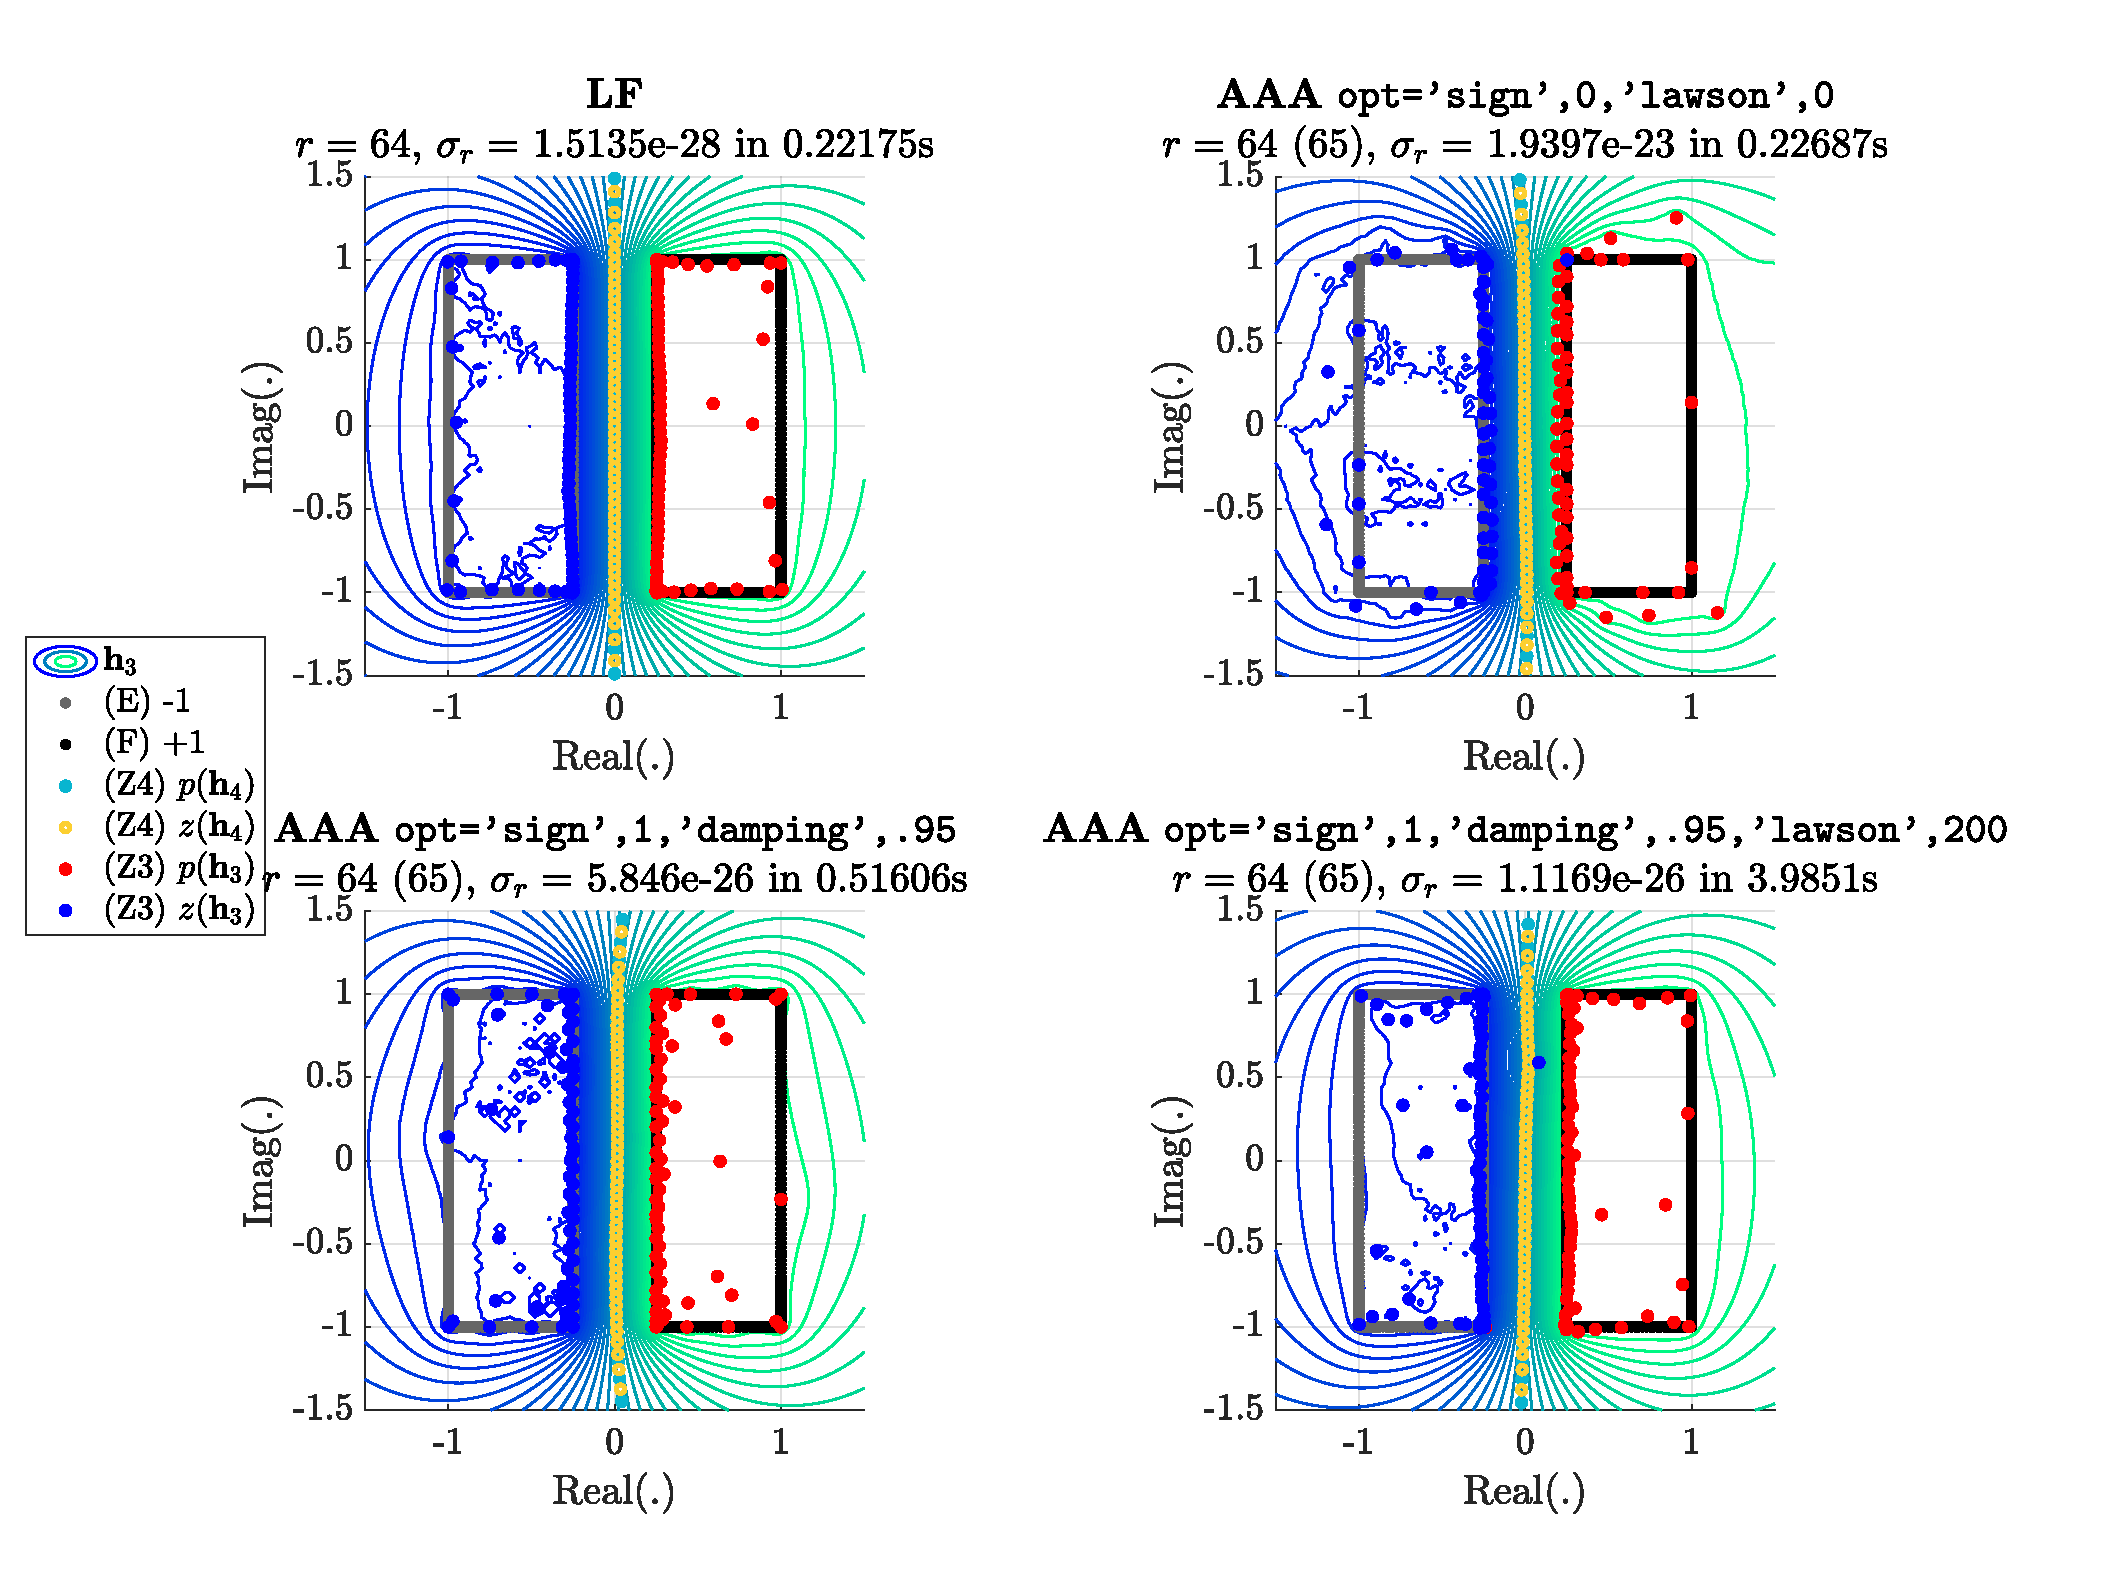
\includegraphics[width=.75\textwidth,align=c]{figures/all/cas_7_r1e-14.pdf}
    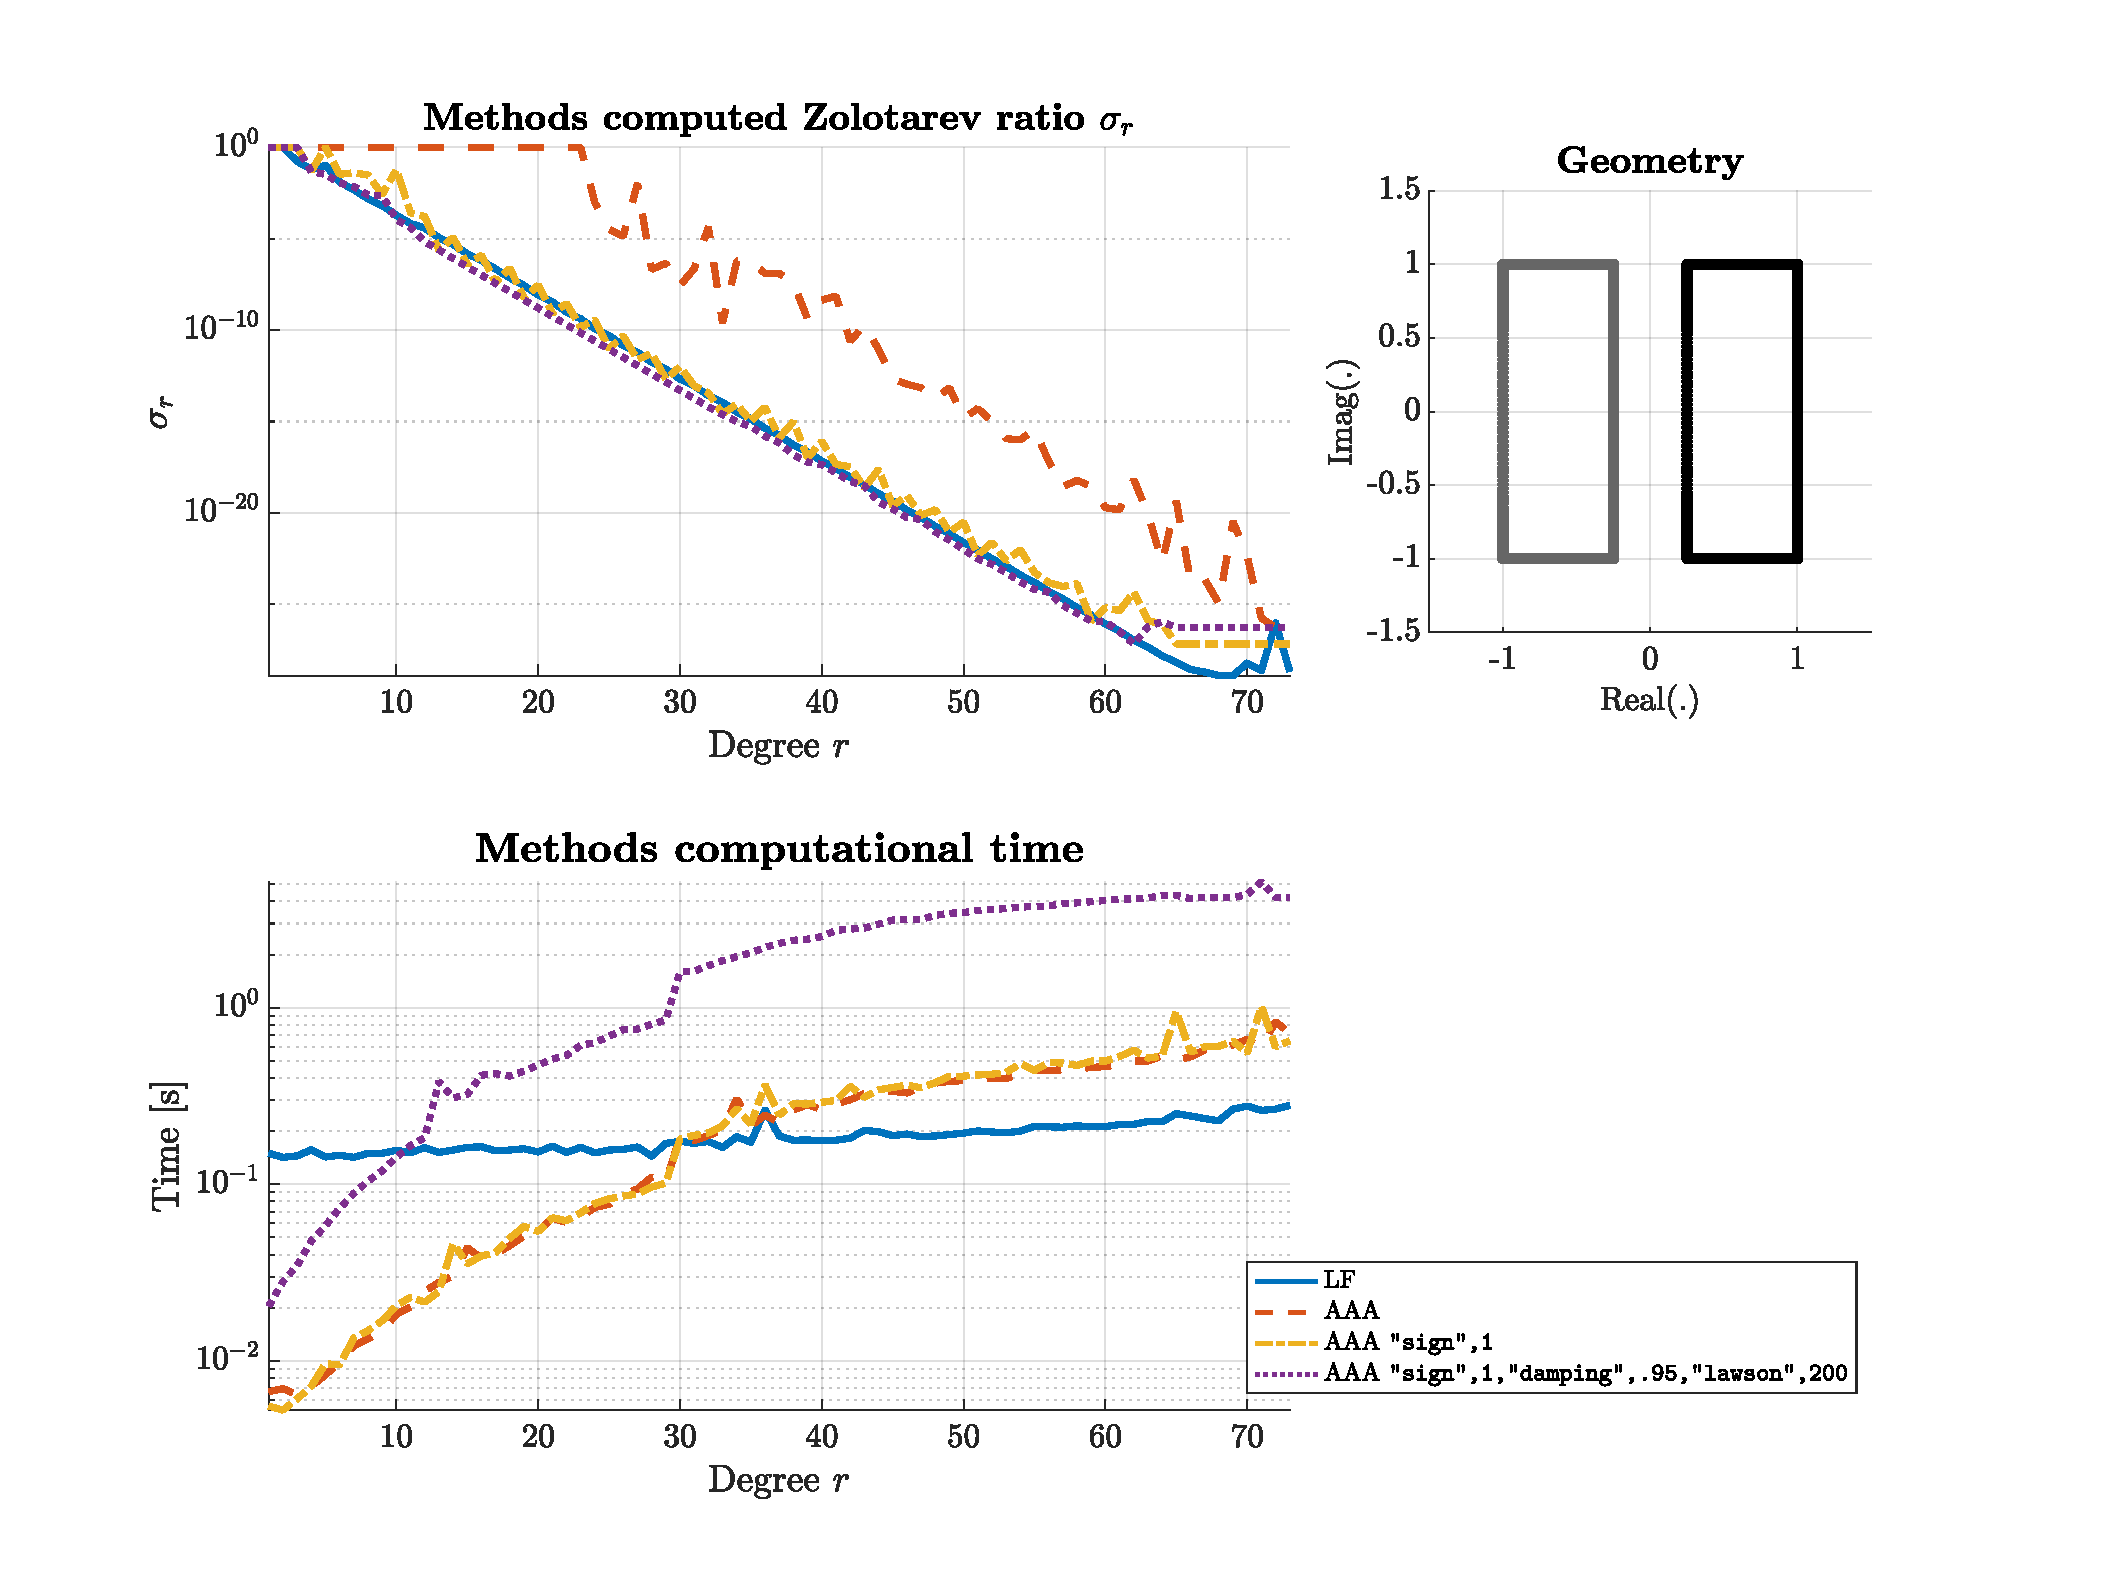
\includegraphics[width=.75\textwidth,align=c]{figures/time_accuracy/cas_7_zol_time.pdf}
    \caption{Case \texttt{'7'}. Top: same description as \cref{fig:intro:1a}. Bottom: same description as \cref{fig:intro:1a_time}.}
    \label{fig:7}
\end{figure}

%%%%%%%%%%%%
\newpage
\subsection{Case \texttt{'spiral1'}}

The spiral example shown in \cref{fig:spiral1} (here computed with an LF normalized singular values threshold at $10^{-12}$) illustrates a configuration where again the LF outperforms in all situations, with a lower Zolotarev number, a lower computational time. Moreover, inspecting the upper part of \cref{fig:spiral1}, for the LF, only 2 poles and zeros seem out of the pattern, while the different AAA lead to a large number of irregularly spread poles and zeros. This lets us believe that the LF is able to recover the true structure of the optimal rational approximation.

\begin{figure}[H]
    \centering
    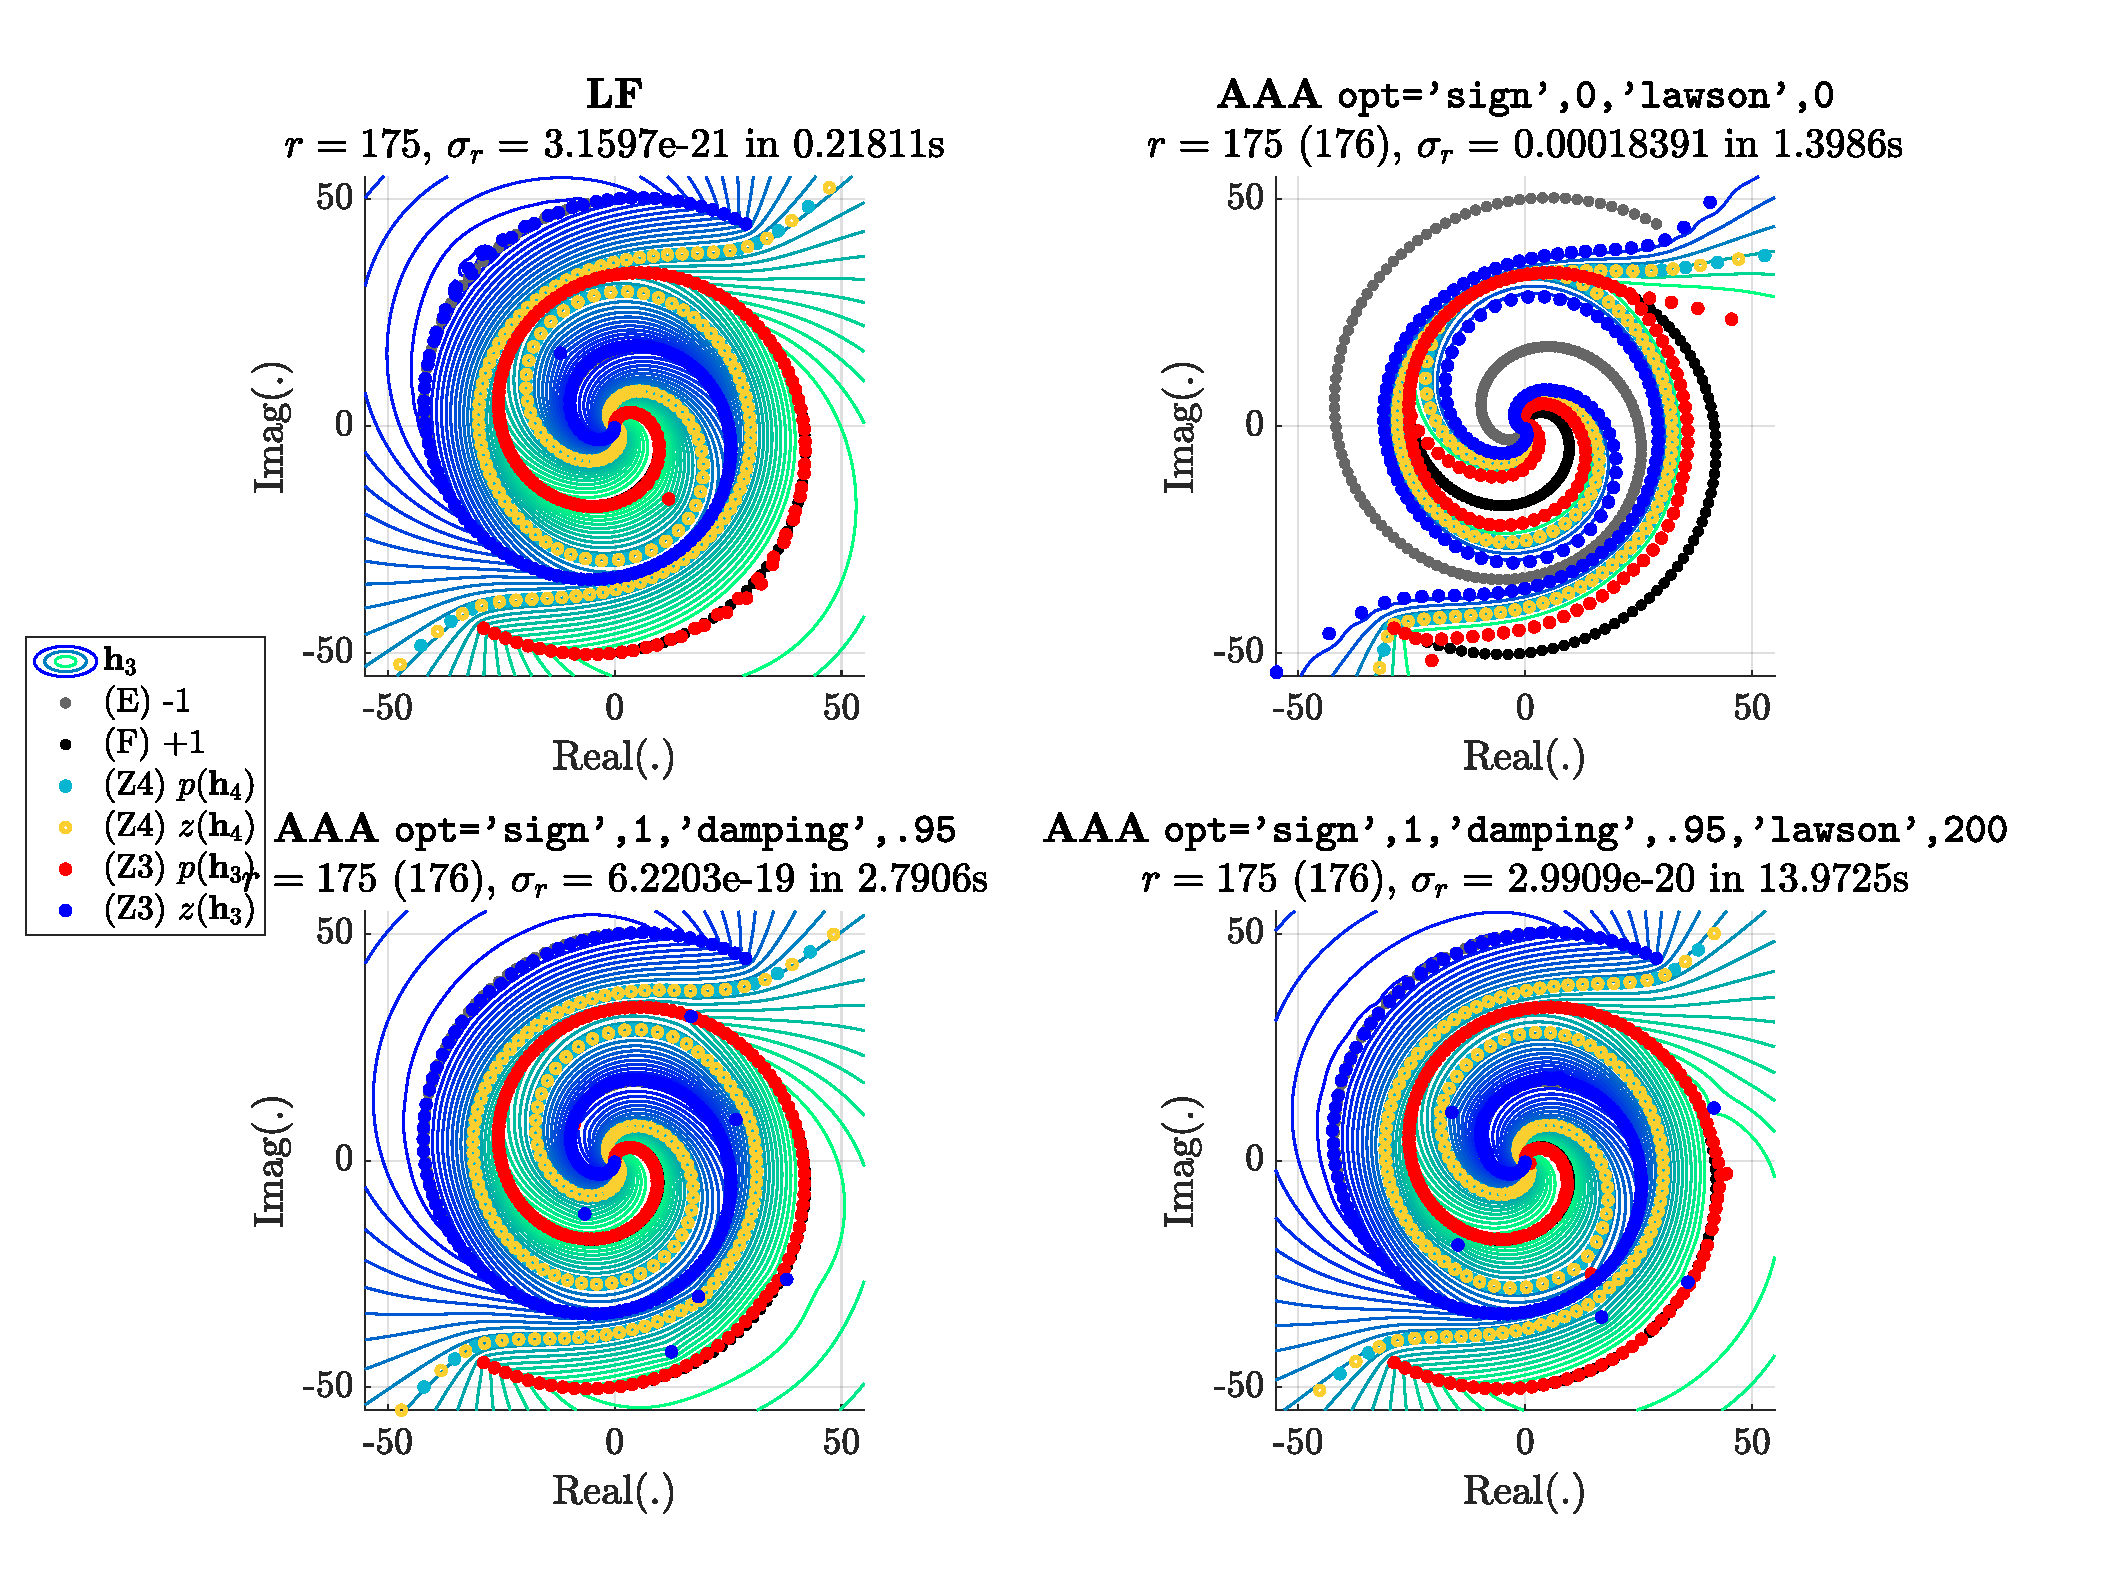
\includegraphics[width=.75\textwidth,align=c]{figures/all/cas_spiral1_r1e-12.pdf}
    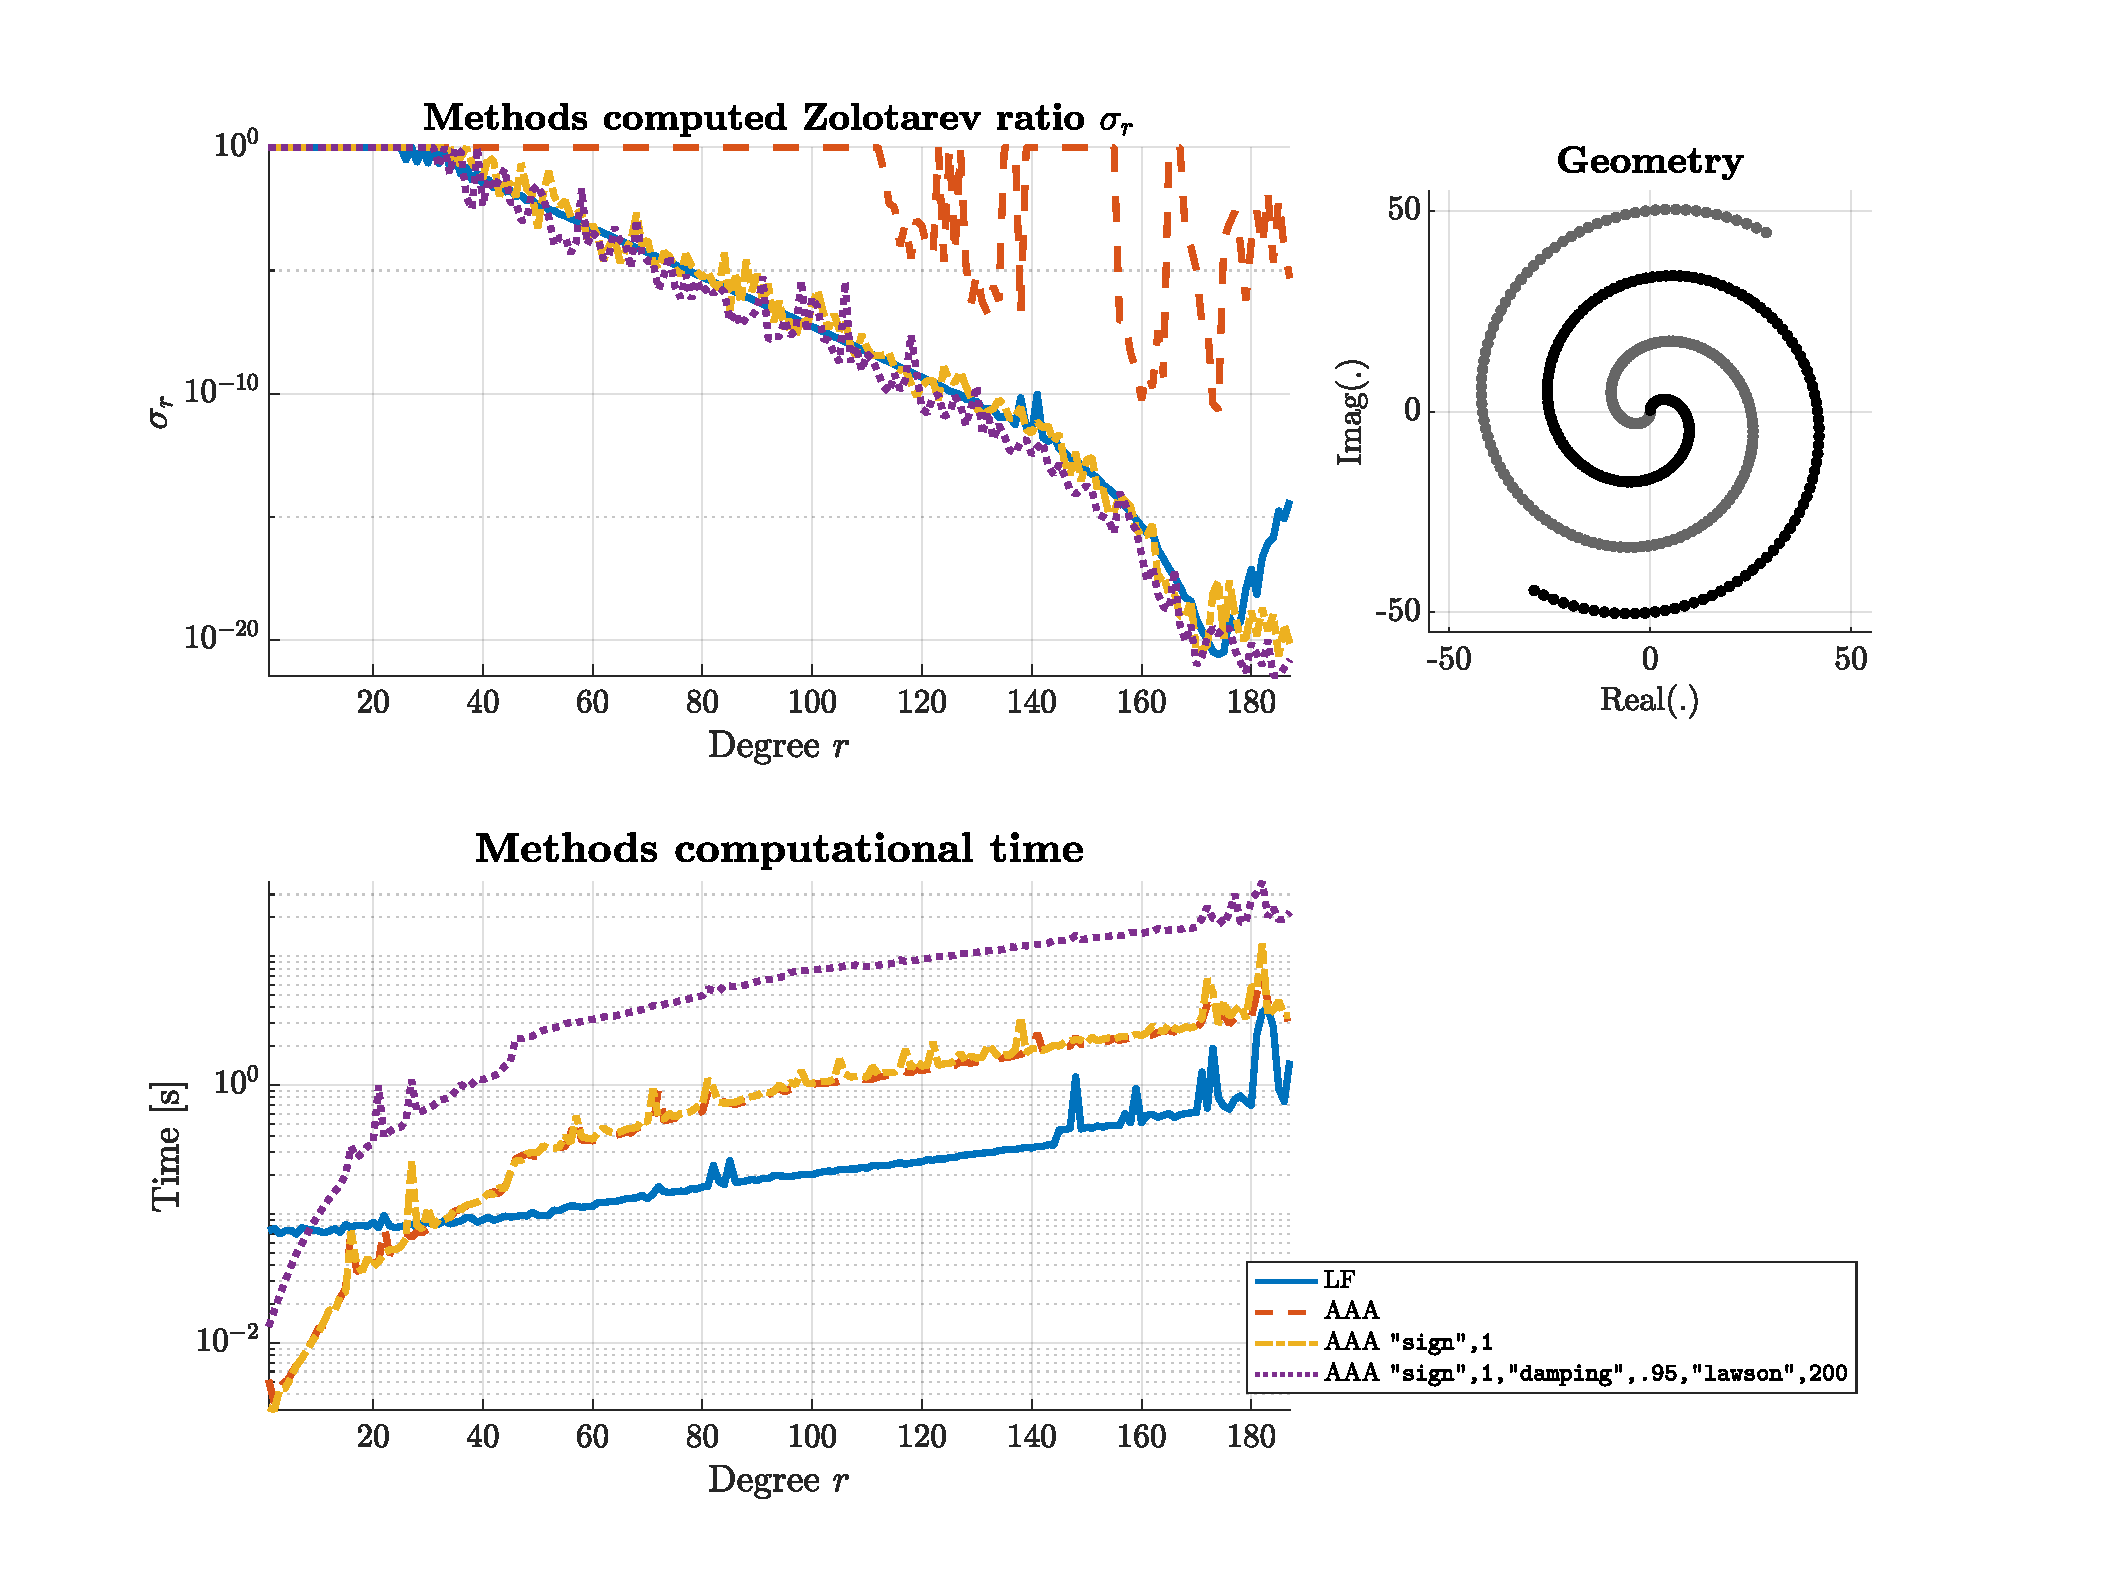
\includegraphics[width=.75\textwidth,align=c]{figures/time_accuracy/cas_spiral1_zol_time.pdf}
    \caption{Case \texttt{'spiral1'}. Top: same description as \cref{fig:intro:1a}. Bottom: same description as \cref{fig:intro:1a_time}.}
    \label{fig:spiral1}
\end{figure}

%%%%%%%%%%%%
\newpage
\subsection{Case \texttt{'pm2'}}

The last configuration in \cref{fig:pm2} shows the Pac-Man figure (to the left) from the homonymous video game in the 80s \footnote{More details here: \url{https://pacman.com/en/history/}}, seeking to eat a candy depicted as a disk (on the right). Similar comments hold with almost the same accuracy between LF, AAA sign, and AAA sign Lawson, but with a significantly lower computation time for LF. Again, the nicely symmetric and well-distributed poles and zeros are obtained by the LF methodology only.

\begin{figure}[H]
    \centering
    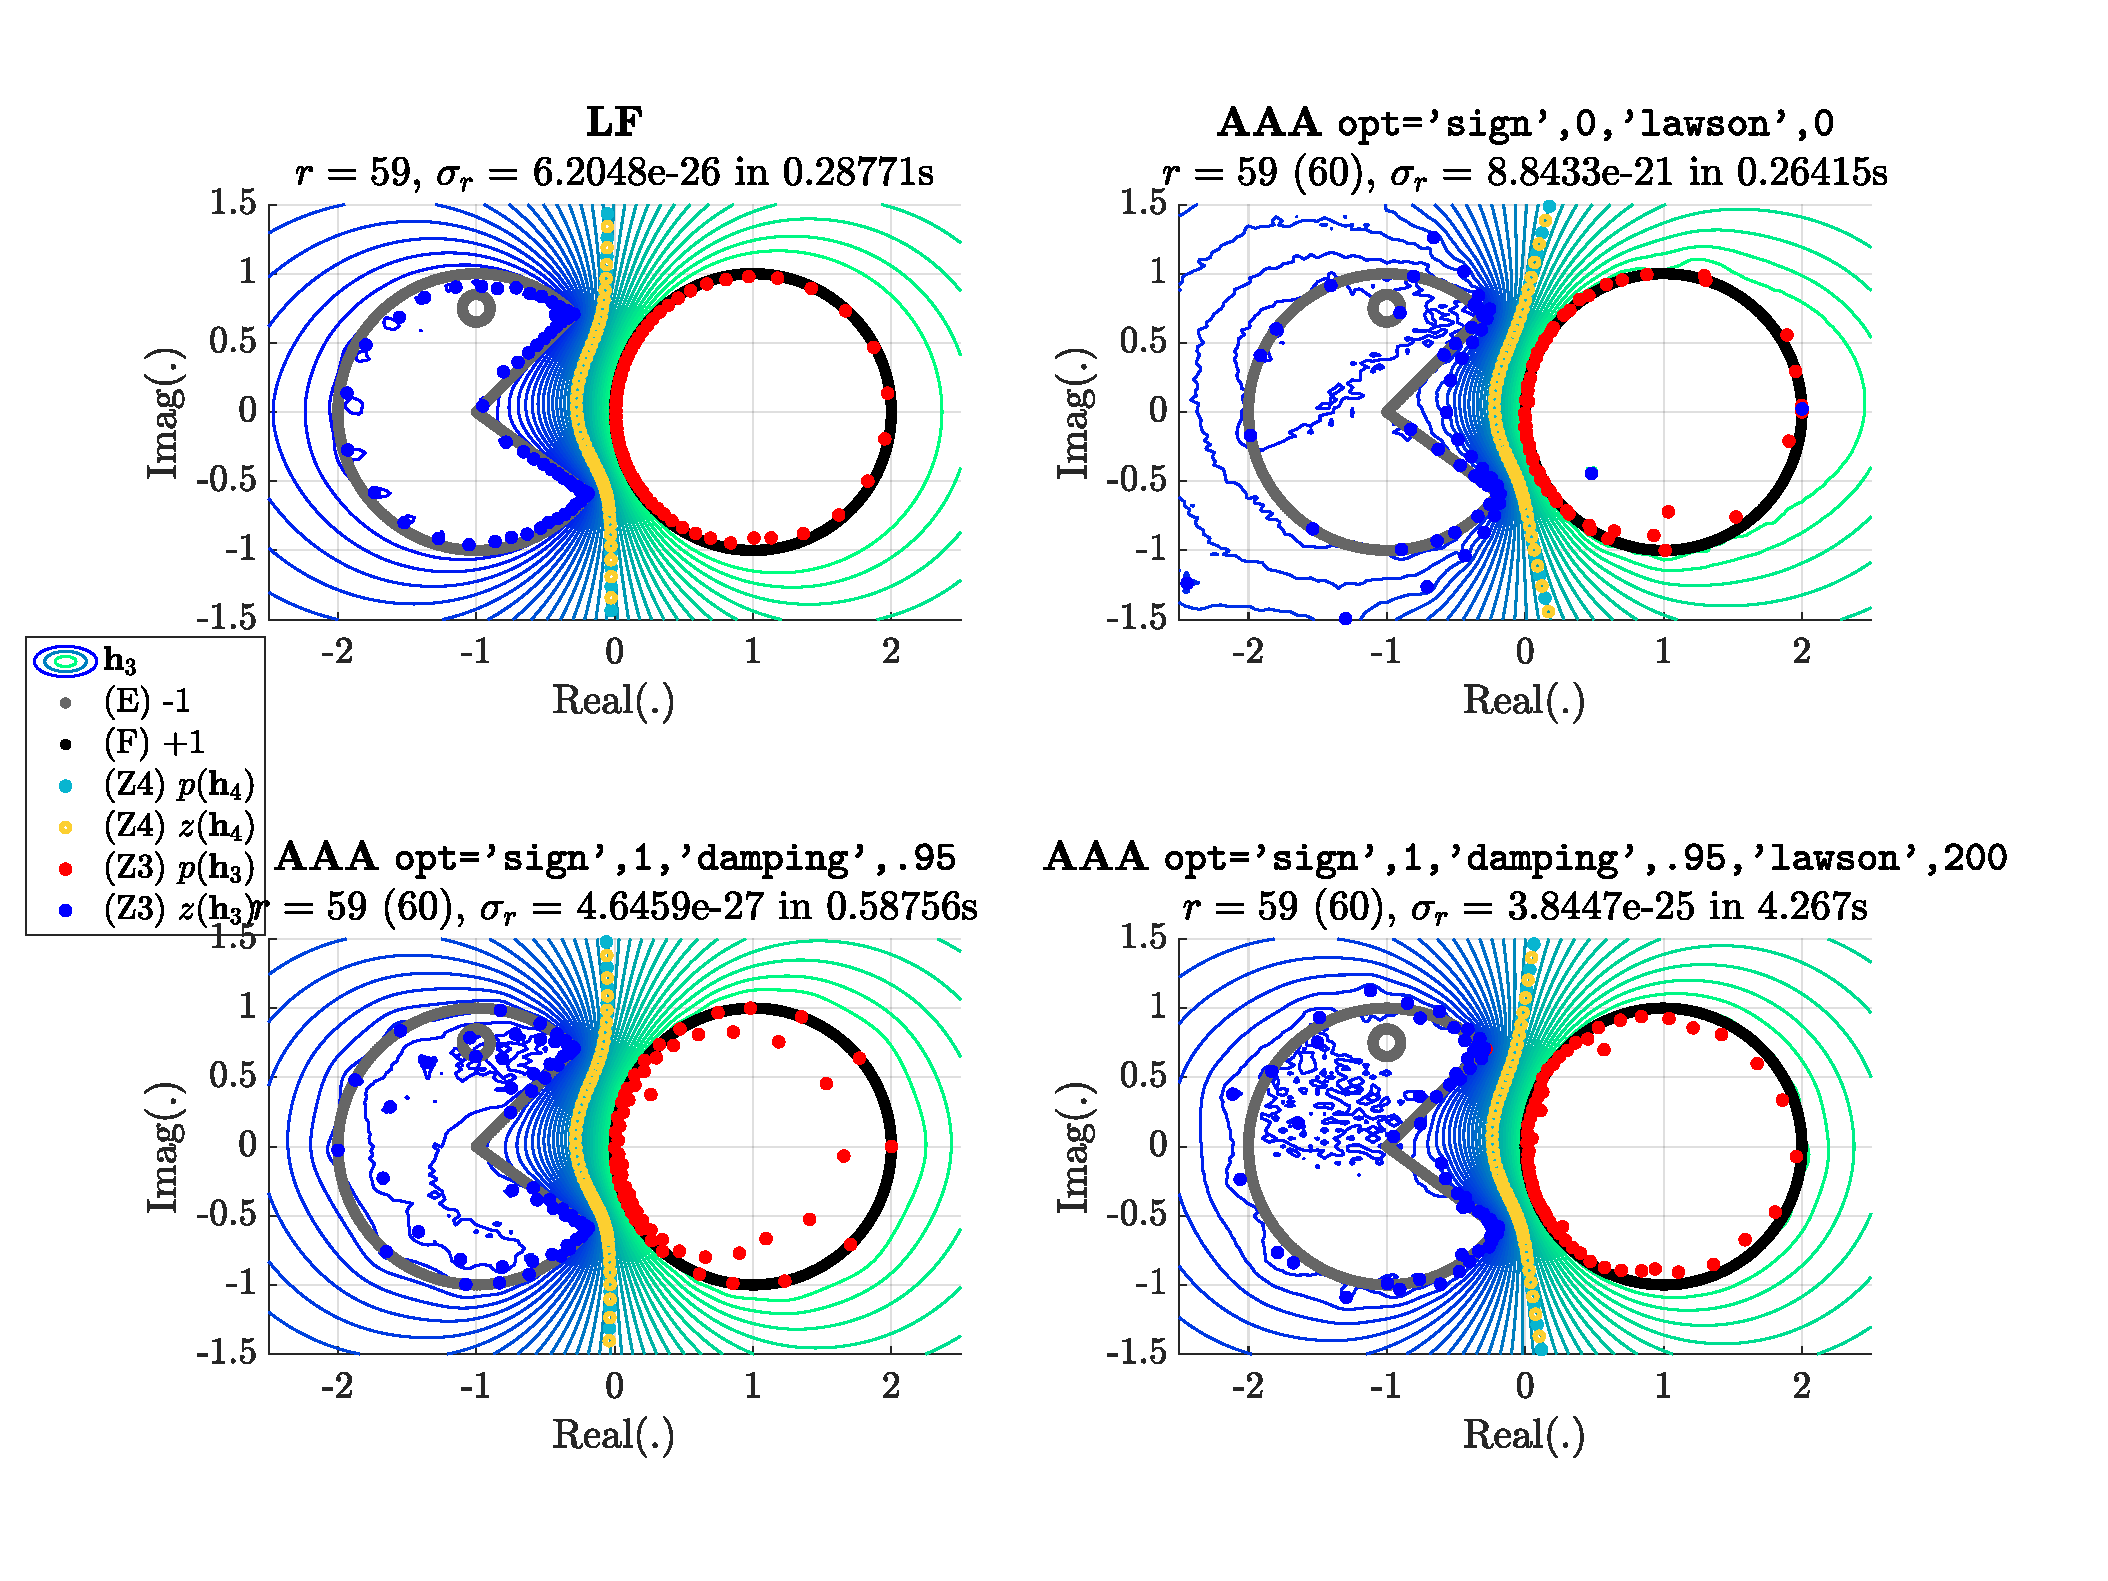
\includegraphics[width=.75\textwidth,align=c]{figures/all/cas_pm2_r1e-14.pdf}
    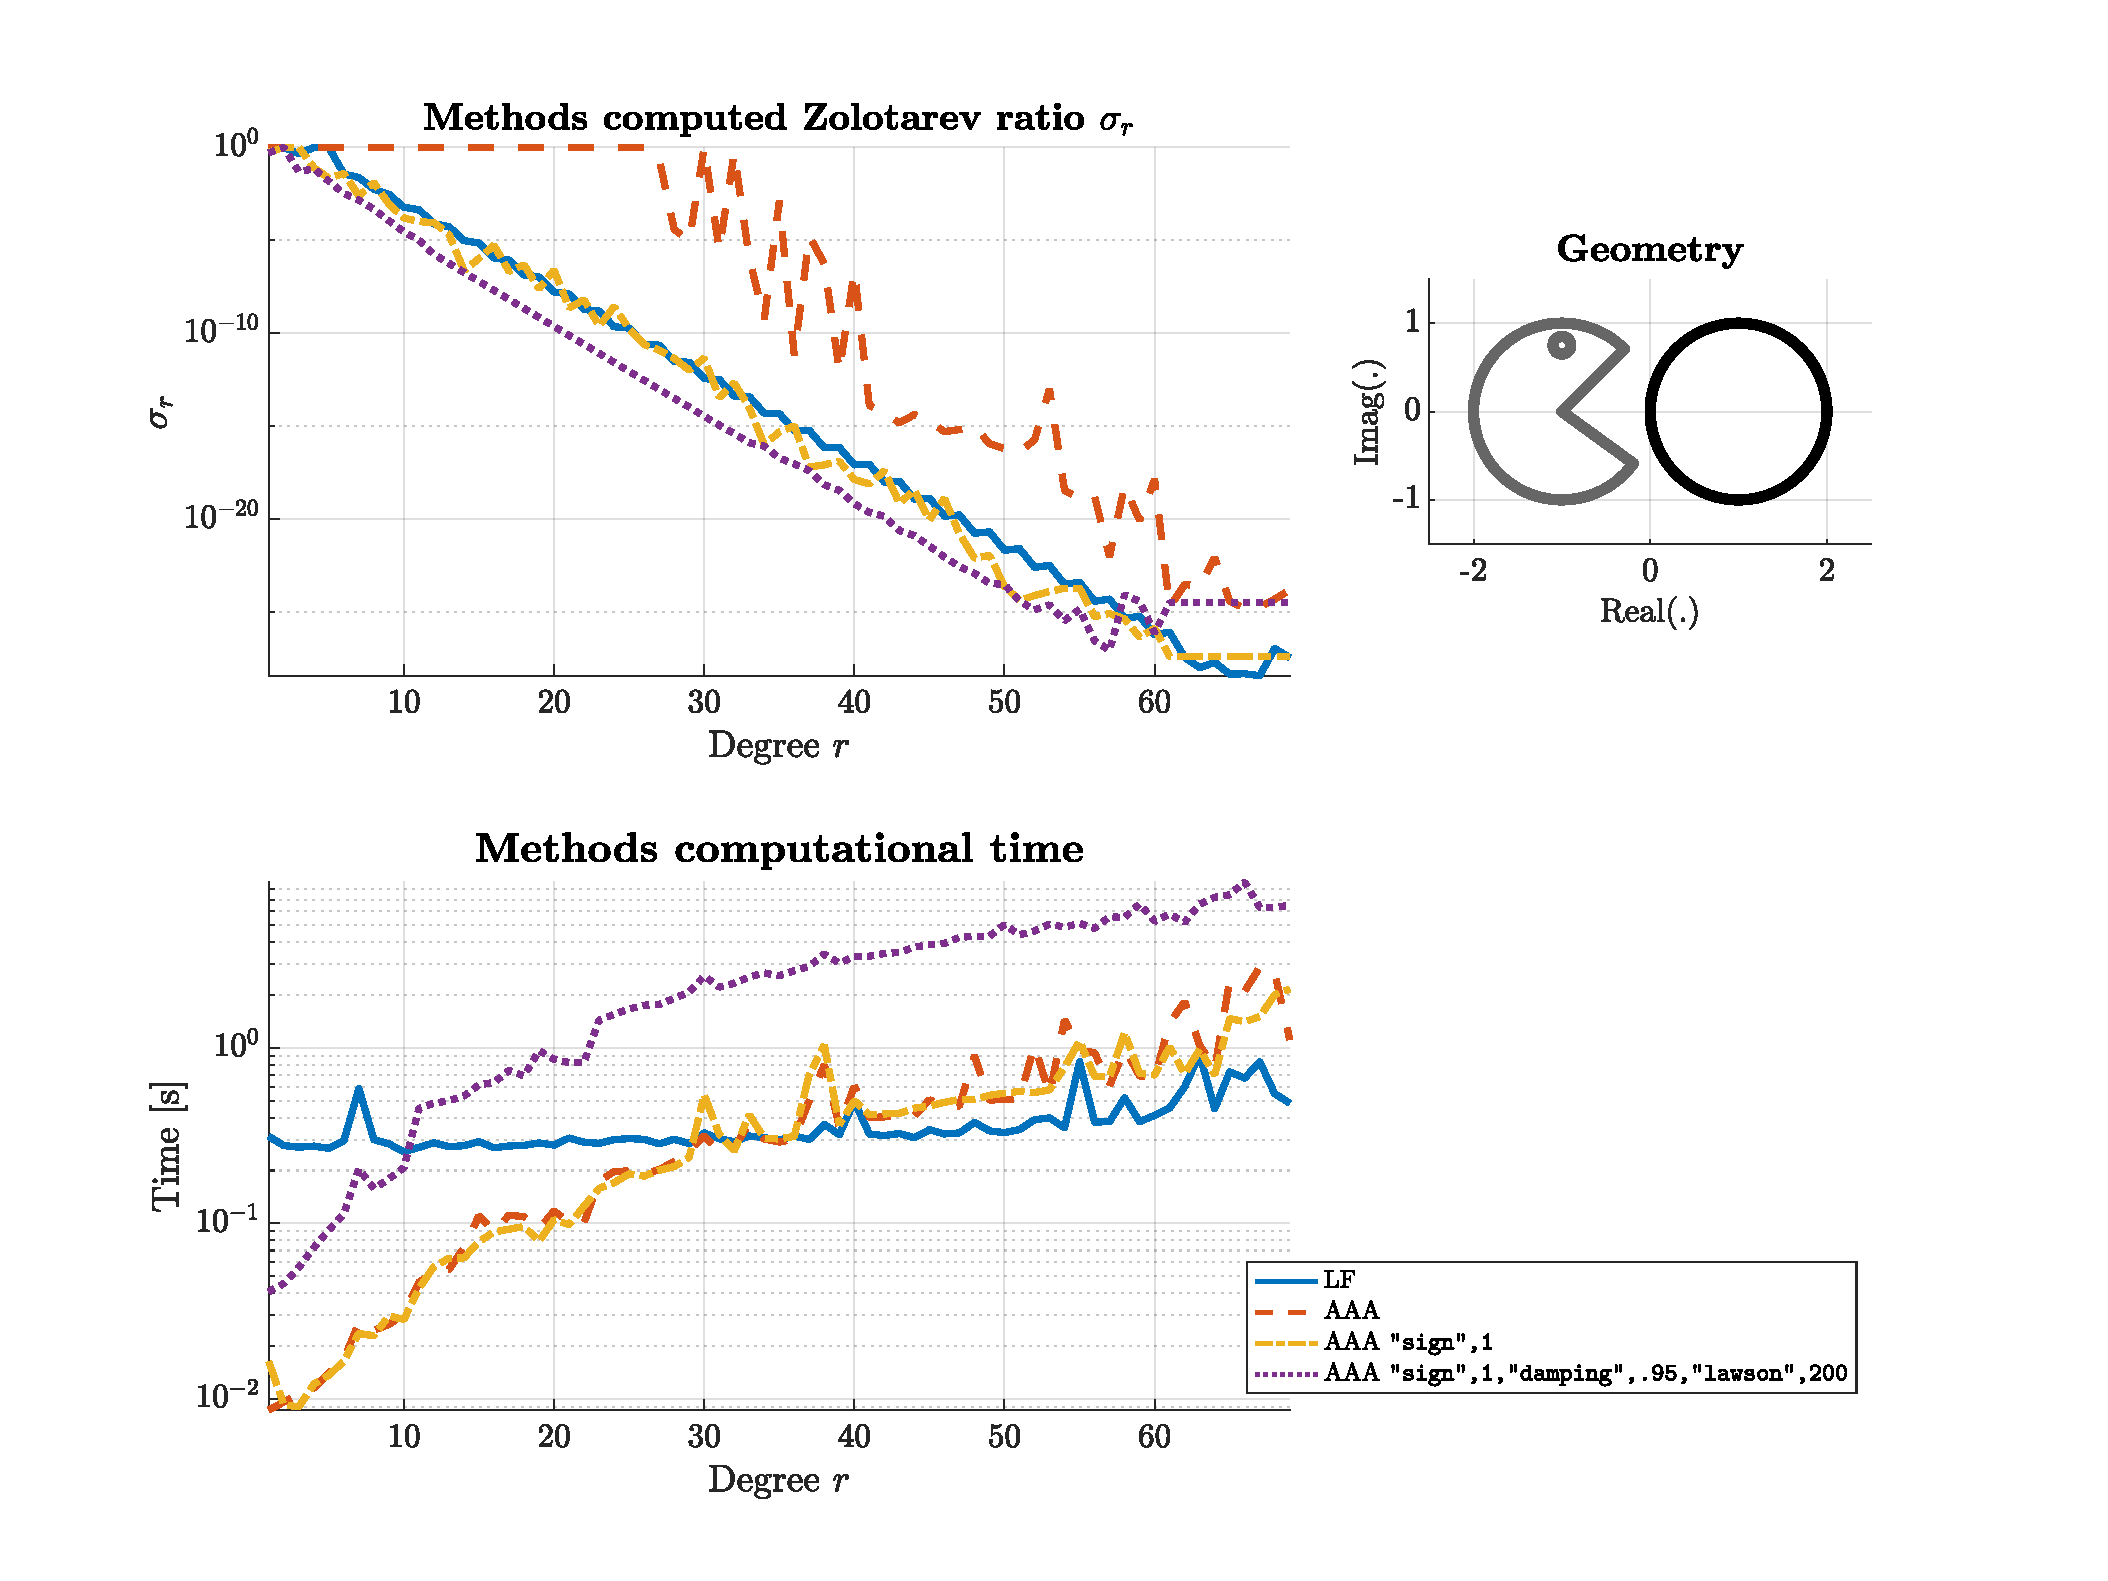
\includegraphics[width=.75\textwidth,align=c]{figures/time_accuracy/cas_pm2_zol_time.pdf}
    \caption{Case \texttt{'pm2'}. Top: same description as \cref{fig:intro:1a}. Bottom: same description as \cref{fig:intro:1a_time}.}
    \label{fig:pm2}
\end{figure}

